% ============================================================
% MÉMOIRE DE FIN D'ÉTUDES — MASTER 2 IA EMBARQUÉE
% FSA Aït Melloul — Université Ibn Zohr — 2024/2025
% ============================================================

\documentclass[12pt, a4paper, oneside]{report}

% ── Langues et polices ──────────────────────────────────────
\usepackage{iftex}
\ifPDFTeX
  \usepackage[utf8]{inputenc}
  \usepackage[T1]{fontenc}
  \usepackage[french]{babel}
  \usepackage{lmodern}
  \makeatletter
  \providecommand{\xpg@aux}[2]{}
  \makeatother
\else
  \usepackage{fontspec}
  \usepackage{polyglossia}
  \setmainlanguage{french}
  \setotherlanguage{arabic}
  \setmainfont{Latin Modern Roman}[
    SmallCapsFont = {Latin Modern Roman Caps}
  ]
  \newfontfamily\arabicfont[
    Script = Arabic,
    Scale  = 1.2
  ]{Amiri}
\fi
\usepackage{csquotes}

% ── Mise en page ─────────────────────────────────────────────
\usepackage[
  top=2.5cm, bottom=2.5cm,
  left=3cm,  right=2.5cm
]{geometry}
\usepackage{setspace}
\onehalfspacing
\hbadness=10000
\hfuzz=20pt
\emergencystretch=3em

% ── Couleurs ─────────────────────────────────────────────────
\usepackage[dvipsnames, table]{xcolor}

% Palette couleurs du projet
\definecolor{PrimaryBlue}  {RGB}{0,  82,  155}
\definecolor{AccentGreen}  {RGB}{0,  150,  80}
\definecolor{AccentOrange} {RGB}{220, 100,  0}
\definecolor{LightGray}    {RGB}{245, 245, 245}
\definecolor{DarkGray}     {RGB}{80,  80,  80}
\definecolor{CodeBG}       {RGB}{248, 248, 248}

% ── Graphiques et figures ─────────────────────────────────────
\usepackage{graphicx}
\usepackage{float}
\usepackage{caption}
\usepackage{subcaption}
\usepackage{wrapfig}
\graphicspath{{figures/}}
\DeclareGraphicsExtensions{.pdf,.png,.jpg,.jpeg}

% ── Blocs colorés ────────────────────────────────────────────
\usepackage{tcolorbox}
\tcbuselibrary{skins, breakable, listings}

% Bloc définition
\newtcolorbox{definitionbox}[1]{
  colback  = PrimaryBlue!8,
  colframe = PrimaryBlue,
  fonttitle= \bfseries\color{white},
  title    = {#1},
  arc      = 4pt
}

% Bloc résultat/contribution
\newtcolorbox{resultbox}[1]{
  colback  = AccentGreen!8,
  colframe = AccentGreen,
  fonttitle= \bfseries\color{white},
  title    = {#1},
  arc      = 4pt
}

% Bloc attention/limite
\newtcolorbox{warningbox}[1]{
  colback  = AccentOrange!8,
  colframe = AccentOrange,
  fonttitle= \bfseries\color{white},
  title    = {#1},
  arc      = 4pt
}

% ── Tableaux ──────────────────────────────────────────────────
\usepackage{booktabs}
\usepackage{multirow}
\usepackage{tabularx}
\usepackage{array}
\usepackage{longtable}

% ── Diagrammes TikZ ──────────────────────────────────────────
\usepackage{tikz}
\usepackage{pgfplots}
\pgfplotsset{compat=1.18}
\usetikzlibrary{
  shapes.geometric,
  arrows.meta,
  positioning,
  fit,
  backgrounds,
  shadows
}

% ── Algorithmes ───────────────────────────────────────────────
\usepackage{algorithm}
\usepackage{algorithmic}

% ── Code source ───────────────────────────────────────────────
\usepackage{listings}
\lstset{
  backgroundcolor = \color{CodeBG},
  basicstyle      = \ttfamily\footnotesize,
  keywordstyle    = \color{PrimaryBlue}\bfseries,
  commentstyle    = \color{DarkGray}\itshape,
  stringstyle     = \color{AccentGreen},
  numbers         = left,
  numberstyle     = \tiny\color{DarkGray},
  frame           = single,
  rulecolor       = \color{LightGray},
  breaklines      = true,
  showstringspaces= false,
  tabsize         = 4
}

% ── Mathématiques ─────────────────────────────────────────────
\usepackage{amsmath}
\usepackage{amssymb}

% ── Liens et références ───────────────────────────────────────
\usepackage[
  colorlinks = true,
  linkcolor  = PrimaryBlue,
  citecolor  = AccentGreen,
  urlcolor   = PrimaryBlue
]{hyperref}
\usepackage[french]{cleveref}

% ── Bibliographie ─────────────────────────────────────────────
\bibliographystyle{ieeetr}

% ── En-têtes et pieds de page ─────────────────────────────────
\usepackage{fancyhdr}
\pagestyle{fancy}
\fancyhf{}
\fancyhead[L]{\small\leftmark}
\fancyhead[R]{\small\thepage}
\renewcommand{\headrulewidth}{0.4pt}
\setlength{\headheight}{16pt}

% ── Chapitres stylisés ────────────────────────────────────────
\usepackage{titlesec}
\titleformat{\chapter}[display]
  {\normalfont\huge\bfseries\color{PrimaryBlue}}
  {\chaptertitlename\ \thechapter}
  {20pt}
  {\Huge}
\titlespacing*{\chapter}{0pt}{-10pt}{30pt}

% ── Acronymes ─────────────────────────────────────────────────
\usepackage{acronym}

% ── Espacement paragraphes ───────────────────────────────────
\setlength{\parskip}{6pt}
\setlength{\parindent}{0pt}

% ============================================================
\begin{document}

% ── Pages préliminaires ──────────────────────────────────────
% ============================================================
% 00_cover.tex — Page de garde
% ============================================================

\hypersetup{pageanchor=false}
\begin{titlepage}
\begin{center}

% ── Logo université ──────────────────────────────────────────

\includegraphics[width=0.24\textwidth]{logo_ibn_zohr}
\hfill

\includegraphics[width=0.24\textwidth]{logo_fsa}

\vspace{0.18cm}
\rule{\linewidth}{0.4pt}

% ── Établissement ────────────────────────────────────────────
{\large\textbf{Université Ibn Zohr}}\\[0.08cm]
{\normalsize Faculté des Sciences Appliquées d'Aït Melloul}\\[0.05cm]
{\normalsize Département Génie Informatique et Systèmes Intelligents}

\rule{\linewidth}{0.4pt}
\vspace{0.18cm}

% ── Type de document ─────────────────────────────────────────
{\large\textcolor{DarkGray}{Mémoire de Fin d'Études}}\\[0.08cm]
{\small Présenté en vue de l'obtention du diplôme de}\\[0.1cm]
{\large\textbf{Master en Intelligence Artificielle Embarquée}}

\vspace{0.25cm}

% ── Titre ────────────────────────────────────────────────────
\begin{tcolorbox}[
  colback  = PrimaryBlue!6,
  colframe = PrimaryBlue,
  arc      = 5pt,
  boxrule  = 1.2pt,
  left     = 6pt,
  right    = 6pt,
  top      = 6pt,
  bottom   = 6pt
]
\begin{center}
{\LARGE\bfseries\color{PrimaryBlue}
Gestion Intelligente des Feux de Circulation}\\[0.12cm]
{\large\bfseries\color{PrimaryBlue}
dans une Smart City via Edge AI}\\[0.18cm]
{\normalsize\bfseries\color{DarkGray}
Détection Multi-Classes, Anonymisation Temps Réel}\\[0.06cm]
{\normalsize\bfseries\color{DarkGray}
et Décision Adaptative sur Dispositif Embarqué}
\end{center}
\end{tcolorbox}

\vspace{0.15cm}

% ── Auteur ───────────────────────────────────────────────────
{\small Préparé par}\\[0.12cm]
{\Large\bfseries Mouad ASSARGUAL}

\vspace{0.35cm}

% ── Jury et encadrement ─────────────────────────────────────
{\small\textbf{Soutenu le \dots Juin 2026, devant le Jury :}}\\[0.08cm]

\begin{center}
\begin{tabular}{p{0.56\textwidth}r}
{\small Pr. El Mehdi \textbf{CHERRAT}} & {\small Encadrant}\\[0.08cm]
{\small Pr. \_\_\_\_\_\_\_\_\_\_\_\_\_} & {\small Examinateur}\\[0.08cm]
{\small Pr. \_\_\_\_\_\_\_\_\_\_\_\_\_} & {\small Rapporteur}\\[0.08cm]
{\small Pr. \_\_\_\_\_\_\_\_\_\_\_\_\_} & {\small Président du jury}
\end{tabular}
\end{center}

\vspace{0.85cm}

% ── Bas de page ──────────────────────────────────────────────
\rule{\linewidth}{0.4pt}
{\normalsize Année Universitaire \textbf{2025 -- 2026}}

\end{center}
\end{titlepage}
\clearpage
\hypersetup{pageanchor=true}
% ============================================================
% 01_dedication.tex — Dédicace
% ============================================================

\newpage
\thispagestyle{empty}


\begin{flushright}

{\large\textit{À mes très chers parents,}}\\[0.3cm]
{\normalsize\textit{qui ont tout sacrifié pour que je devienne}}\\
{\normalsize\textit{la meilleure version de moi-même.}}\\
{\normalsize\textit{Aucun mot ne pourra jamais exprimer}}\\
{\normalsize\textit{ma gratitude et mon amour.}}

\vspace{0.25cm}

{\large\textit{À ma famille,}}\\[0.2cm]
{\normalsize\textit{mon refuge et ma force dans les moments difficiles.}}

\vspace{0.45cm}

{\large\textit{À mes professeurs,}}\\[0.2cm]
{\normalsize\textit{que je respecte profondément et qui n'ont jamais}}\\
{\normalsize\textit{cessé de nous guider avec bienveillance et dévouement.}}

\vspace{0.45cm}

{\large\textit{À mon encadrant, M. El Mehdi CHERRAT,}}\\[0.2cm]
{\normalsize\textit{pour sa confiance, sa patience et ses précieux conseils}}\\
{\normalsize\textit{qui ont façonné ce travail.}}

\vspace{0.45cm}

{\large\textit{À mes amis et collègues,}}\\[0.2cm]
{\normalsize\textit{compagnons de route qui ont rendu ce parcours}}\\
{\normalsize\textit{plus léger et plus humain.}}

\vspace{0.45cm}

{\large\textit{À toute personne qui m'a tendu la main,}}\\[0.2cm]
{\normalsize\textit{de près ou de loin, un jour dans ma vie.}}

\vspace{0.45cm}

\begin{tcolorbox}[
  colback  = PrimaryBlue!8,
  colframe = PrimaryBlue,
  arc      = 4pt,
  width    = 0.85\textwidth
]
\begin{center}
{\normalsize\textit{Et à ceux qui ont dressé des obstacles sur mon chemin,}}\\[0.2cm]
{\normalsize\textit{vous m'avez appris que la résilience}}\\
{\normalsize\textit{est la plus grande des forces.}}\\[0.3cm]
{\small\textcolor{PrimaryBlue}{\textbf{— Ce travail est le fruit de tout cela.}}}
\end{center}
\end{tcolorbox}

\vspace{0.7cm}

{\large\textbf{Mouad ASSARGUAL}}

\end{flushright}
% ============================================================
% 02_acknowledgments.tex — Remerciements
% ============================================================

\newpage
\thispagestyle{empty}

\begin{center}
{\Large\bfseries\color{PrimaryBlue} Remerciements}
\end{center}

\vspace{0.5cm}
\rule{\linewidth}{0.4pt}
\vspace{0.5cm}

{\normalsize

En premier lieu, je rends grâce à \textbf{Allah}, le
Tout-Puissant, qui m'a accordé la santé, la volonté et
la patience nécessaires pour mener à bien ce travail.
C'est par Sa grâce que j'ai pu franchir chaque étape
de ce parcours.

\vspace{0.3cm}

Je tiens à exprimer ma profonde gratitude à mon encadrant,
\textbf{M. El Mehdi CHERRAT}, pour la confiance qu'il
m'a accordée dès le premier jour, pour ses conseils avisés,
sa disponibilité constante et ses encouragements qui m'ont
guidé tout au long de ce projet. Ce travail n'aurait pas
été ce qu'il est sans son accompagnement.

\vspace{0.3cm}

Je souhaite également adresser mes sincères remerciements
à l'ensemble du \textbf{corps professoral et administratif}
de la Faculté des Sciences Appliquées d'Aït Melloul pour
la qualité de l'enseignement dispensé et leur dévouement.
Les connaissances transmises constituent les fondations
sur lesquelles repose ce travail.

\vspace{0.3cm}

Une mention particulière à mes \textbf{collègues de la
promotion Master Intelligence Artificielle Embarquée} —
devenus une véritable famille au fil de ces années.
Ensemble, nous avons traversé les défis, partagé les
doutes et célébré les réussites. Merci pour cette
fraternité sincère.

\vspace{0.3cm}

J'exprime enfin toute ma reconnaissance à \textbf{ma
famille}, pour son soutien indéfectible et ses
encouragements constants qui m'ont donné la force
de persévérer jusqu'au bout.

\vspace{0.3cm}

À tous ceux qui, de près ou de loin, ont contribué
à la réalisation de ce projet — par leurs conseils,
leurs critiques constructives ou simplement leur
présence — je vous adresse mes plus sincères
remerciements.

}

\vspace{0.3cm}
\rule{\linewidth}{0.4pt}

\begin{flushright}
{\normalsize\textit{Mouad ASSARGUAL}}\\
{\small\textit{Aït Melloul, 2026}}
\end{flushright}
% ============================================================
% 03_abstract.tex — Résumés
% ============================================================

% ── RÉSUMÉ EN FRANÇAIS ───────────────────────────────────────
\newpage
\thispagestyle{empty}

\begin{center}
{\Large\bfseries\color{PrimaryBlue} Résumé}
\end{center}
\vspace{0.3cm}
\rule{\linewidth}{0.4pt}
\vspace{0.3cm}

{\normalsize
Face à la croissance rapide des agglomérations urbaines
marocaines et aux défis croissants de la congestion routière,
ce mémoire présente la conception et le déploiement d'un
système intelligent de gestion adaptative des feux de
circulation pour les villes intelligentes, en intégrant
des contraintes strictes de protection des données
personnelles conformément à la Loi 09-08.

Le système proposé repose sur un pipeline complet déployé
sur Raspberry Pi 5 — un dispositif embarqué à ressources
limitées — et s'articule autour de six modules interconnectés :
acquisition vidéo via OpenCV, détection multi-classes par
YOLO26n optimisé au format ONNX FP32, anonymisation temps réel
par floutage gaussien selon le principe Privacy-by-Design,
suivi des objets par tracker IoU sur zones polygonales,
décision adaptative des phases de feux via un Processus
de Décision Markovien (MDP) à politique déterministe,
et visualisation par un tableau de bord Flask en temps réel.

Un dataset hybride de \textbf{6 761 images} a été constitué
en trois étapes méthodologiques rigoureuses — split sans
fuite de données, renforcement de la classe \textit{person}
via CityPersons, et génération de crops pour les petits
piétons — à partir de sources internationales dont le
\textbf{Bellevue Traffic Video Dataset} et de données
locales collectées à \textbf{Lqliaa, Agadir}.
Un benchmark de six architectures YOLO (nano et small)
sur GPU et sur Raspberry Pi 5 confirme que \textbf{YOLO26n
FP32} atteint \textbf{7,6 FPS réels} sur Pi 5 — meilleur
compromis vitesse/taille parmi les douze configurations
testées. Les variantes small sont empiriquement confirmées
incompatibles avec le temps réel (moins de 3 FPS).

La politique MDP validée sur simulation SUMO démontre
une réduction du temps d'attente moyen de
\textbf{$-51\%$ à $-93\%$} selon le scénario,
par rapport aux feux à cycles fixes.
Les quatre hypothèses de recherche sont confirmées,
démontrant la viabilité d'un pipeline complet
d'intelligence artificielle embarquée pour la gestion
intelligente du trafic urbain, ouvrant la voie à des
déploiements réels dans les smart cities marocaines.
}

\vspace{0.4cm}

\begin{tcolorbox}[
  colback  = LightGray,
  colframe = DarkGray,
  arc      = 3pt,
  boxrule  = 0.5pt
]
\textbf{Mots-clés :} Edge AI, YOLO26n, Raspberry Pi 5,
Gestion du trafic, Smart City, Privacy-by-Design,
Anonymisation, ONNX FP32, Processus de Décision Markovien,
Loi 09-08, Bellevue Traffic Dataset.
\end{tcolorbox}

% ── ABSTRACT EN ANGLAIS ──────────────────────────────────────
\newpage
\thispagestyle{empty}

\begin{center}
{\Large\bfseries\color{PrimaryBlue} Abstract}
\end{center}
\vspace{0.3cm}
\rule{\linewidth}{0.4pt}
\vspace{0.3cm}

{\normalsize
In response to the rapid growth of Moroccan urban areas and
the increasing challenges of road congestion, this thesis
presents the design and deployment of an intelligent adaptive
traffic light management system for smart cities, integrating
strict personal data protection constraints in compliance
with Law 09-08.

The proposed system relies on a complete pipeline deployed
on a Raspberry Pi 5 — a resource-constrained embedded device
— structured around six interconnected modules: video
acquisition via OpenCV, multi-class detection using YOLO26n
in ONNX FP32 format, real-time anonymization through
Gaussian blurring following the Privacy-by-Design principle,
IoU-based object tracking over calibrated polygonal zones,
adaptive traffic phase decision-making via a deterministic
Markov Decision Process (MDP), and real-time visualization
through a Flask dashboard.

A hybrid dataset of \textbf{6,761 images} was built in
three methodological steps — leak-free group-based split,
person class reinforcement via CityPersons, and tiny
person crop generation — combining the
\textbf{Bellevue Traffic Video Dataset} with local data
collected in \textbf{Lqliaa, Agadir}.
A comprehensive benchmark of six YOLO architectures
(nano and small variants) on both GPU and Raspberry Pi 5
empirically confirms that \textbf{YOLO26n FP32} achieves
\textbf{7.6 real FPS} on Pi 5 — the best speed/size
trade-off among the twelve tested configurations.
Small variants are empirically confirmed incompatible
with real-time processing (below 3 FPS on Pi 5).

The MDP policy validated on SUMO simulation demonstrates
a reduction in average waiting time of
\textbf{$-51\%$ to $-93\%$} depending on the scenario,
compared to fixed-cycle traffic lights.
All four research hypotheses are confirmed, demonstrating
the viability of a complete embedded AI pipeline for
intelligent urban traffic management, paving the way
for real deployments in Moroccan smart cities.
}

\vspace{0.4cm}

\begin{tcolorbox}[
  colback  = LightGray,
  colframe = DarkGray,
  arc      = 3pt,
  boxrule  = 0.5pt
]
\textbf{Keywords:} Edge AI, YOLO26n, Raspberry Pi 5,
Traffic Management, Smart City, Privacy-by-Design,
Anonymization, ONNX FP32, Markov Decision Process,
Law 09-08, Bellevue Traffic Dataset.
\end{tcolorbox}

% ── RÉSUMÉ EN ARABE ──────────────────────────────────────────
\ifPDFTeX
\newpage
\thispagestyle{empty}
\begin{center}
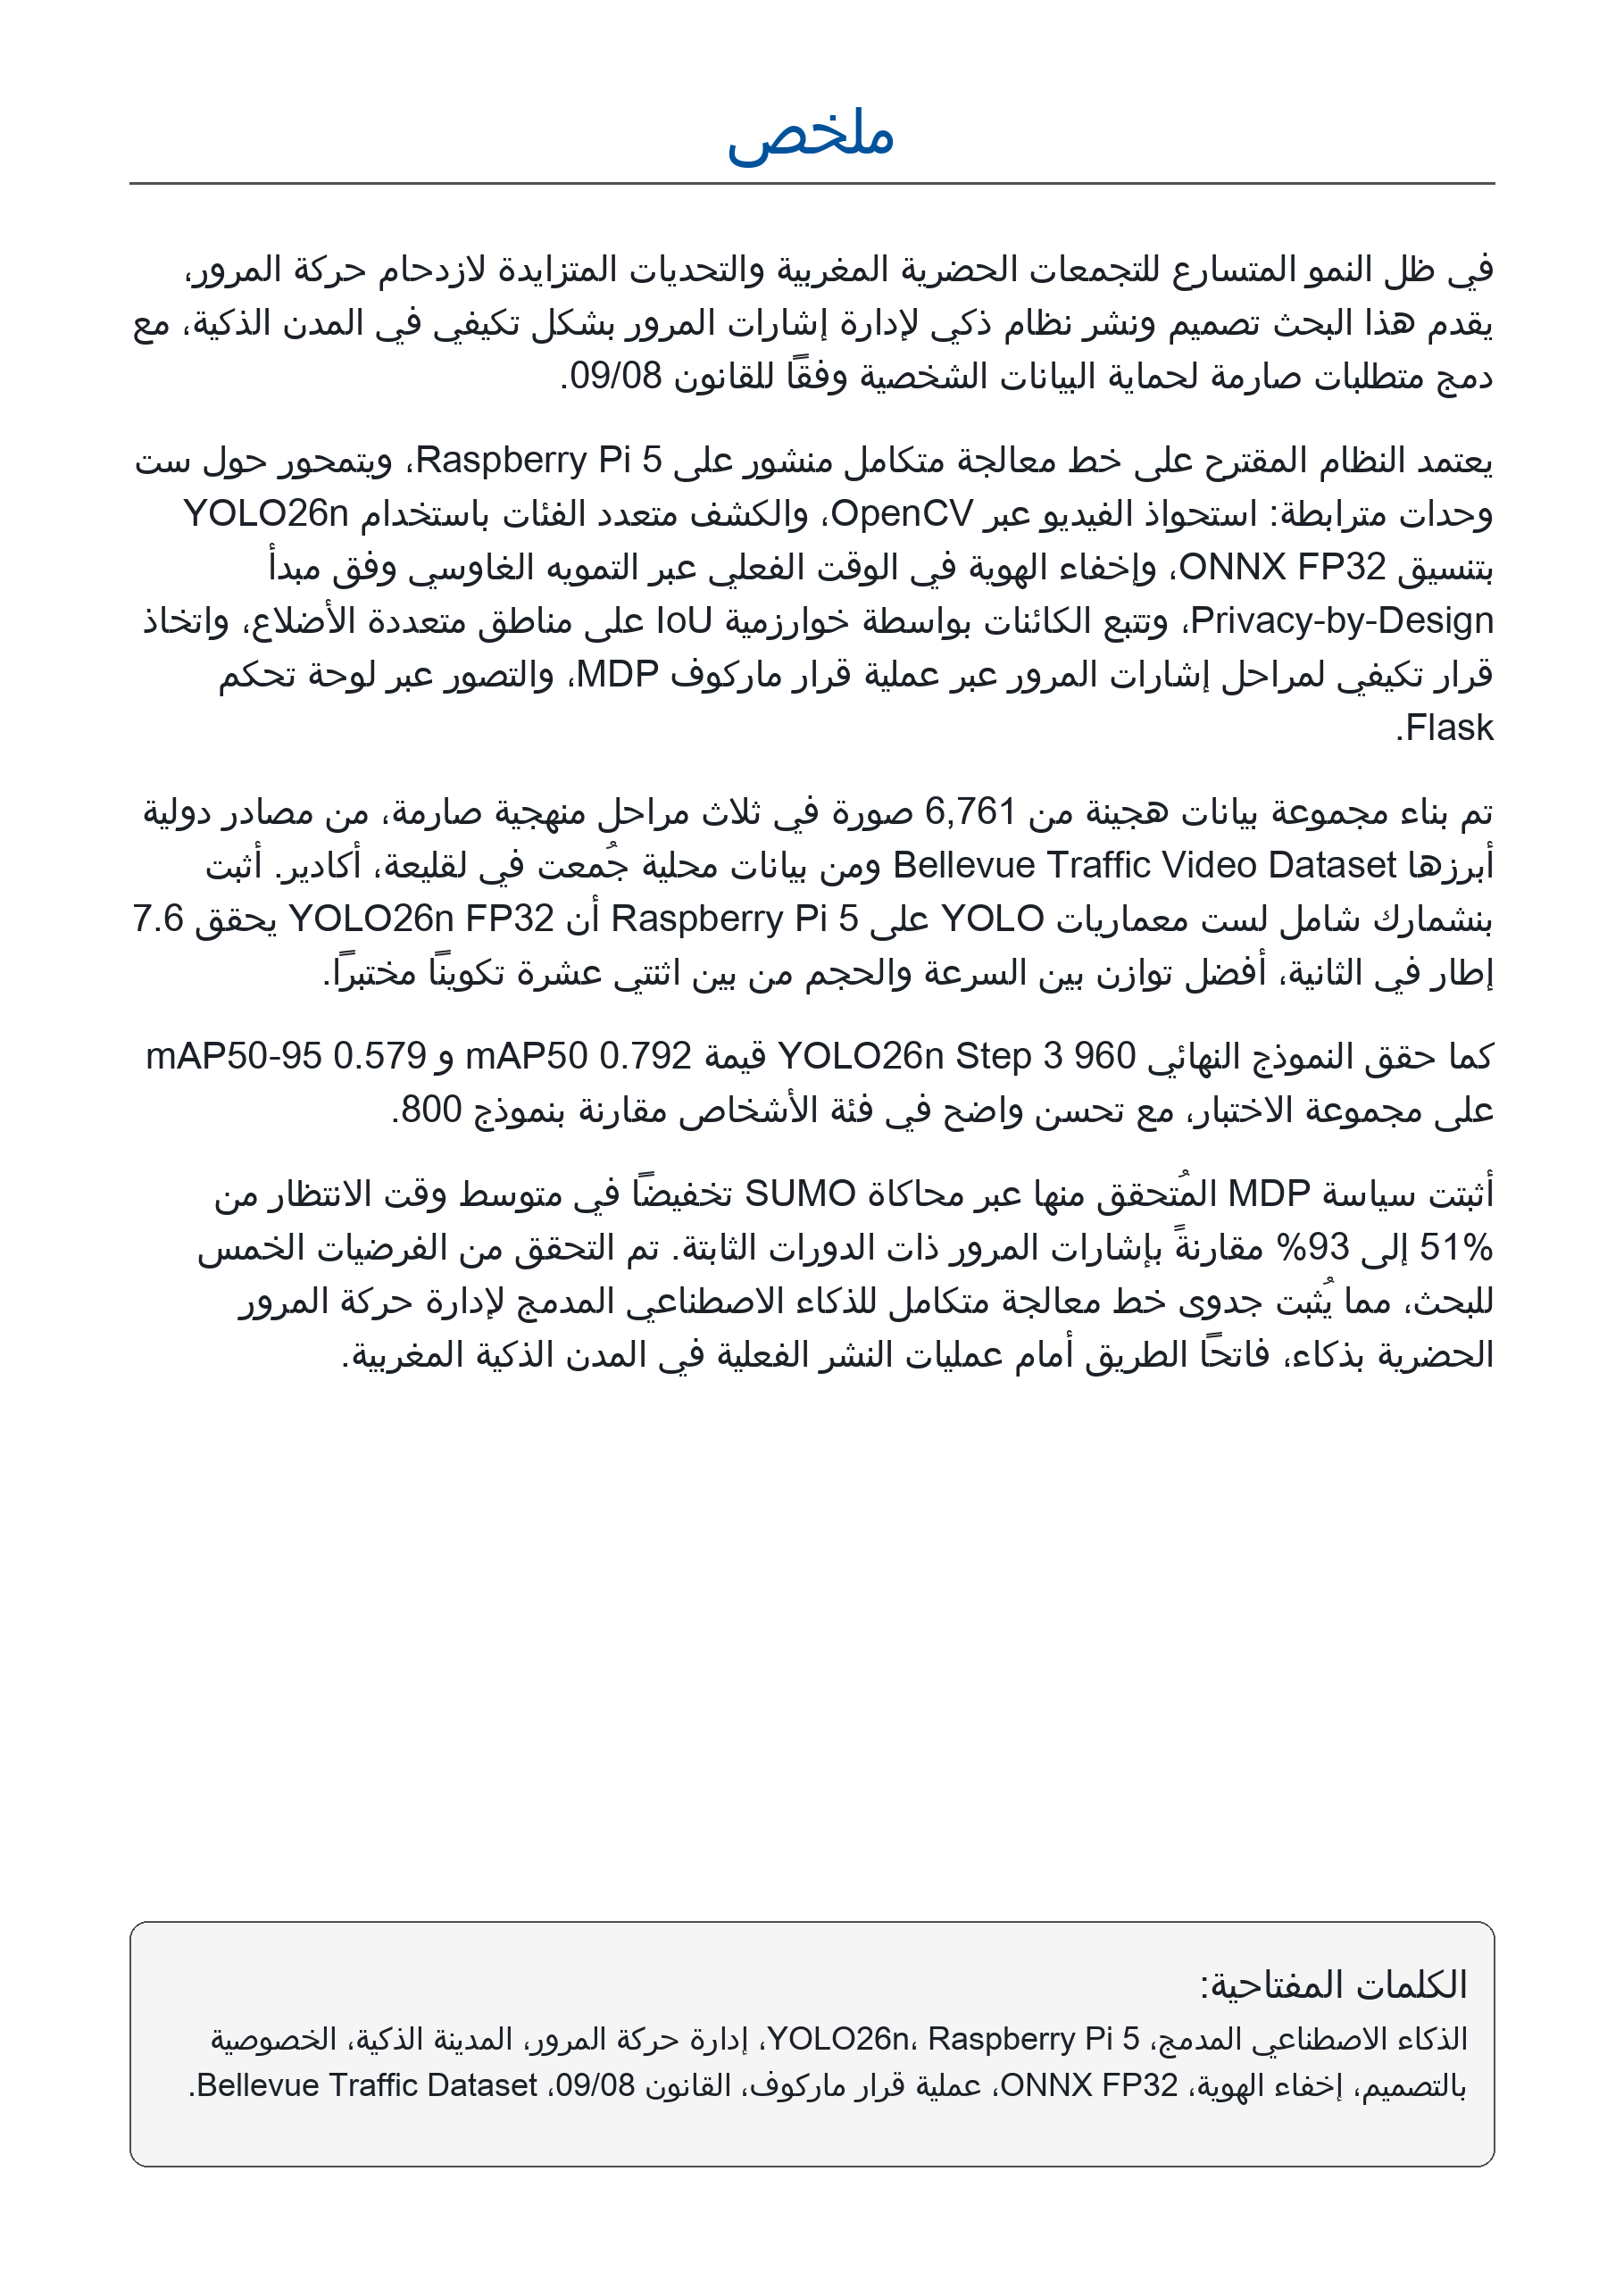
\includegraphics[width=\textwidth,height=0.94\textheight,keepaspectratio]
  {generated/abstract_ar}
\end{center}
\else
\newpage
\thispagestyle{empty}

\begin{center}
{\Large\bfseries\color{PrimaryBlue}
\textarabic{ملخص}}
\end{center}
\vspace{0.3cm}
\rule{\linewidth}{0.4pt}
\vspace{0.3cm}

\begin{Arabic}

في ظل النمو المتسارع للتجمعات الحضرية المغربية
والتحديات المتزايدة لازدحام حركة المرور،
يقدم هذا البحث تصميم ونشر نظام ذكي
لإدارة إشارات المرور بشكل تكيفي في المدن الذكية،
مع دمج متطلبات صارمة لحماية البيانات الشخصية
وفقاً للقانون \LR{09-08}.

يعتمد النظام المقترح على خط معالجة متكامل
منشور على \LR{Raspberry Pi 5}،
ويتمحور حول ستة وحدات مترابطة:
استحواذ الفيديو عبر \LR{OpenCV}،
والكشف متعدد الفئات باستخدام \LR{YOLO26n}
بتنسيق \LR{ONNX FP32}،
وإخفاء الهوية في الوقت الفعلي
عبر التمويه الغاوسي وفق مبدأ
\LR{Privacy-by-Design}،
وتتبع الكائنات بواسطة خوارزمية \LR{IoU}
على مناطق متعددة الأضلاع،
واتخاذ قرار تكيفي لمراحل إشارات المرور
عبر عملية قرار ماركوف \LR{(MDP)}،
والتصور عبر لوحة تحكم \LR{Flask}.

تم بناء مجموعة بيانات هجينة من
\textbf{\LR{6\,761} صورة}
في ثلاث مراحل منهجية صارمة،
من مصادر دولية أبرزها
\LR{Bellevue Traffic Video Dataset}
ومن بيانات محلية جُمعت في
\textbf{لقليعة، أكادير}.
أثبت بنشمارك شامل لست معماريات \LR{YOLO}
على \LR{Raspberry Pi 5}
أن \LR{YOLO26n FP32} يحقق
\textbf{\LR{7.6} إطار في الثانية}،
أفضل توازن بين السرعة والحجم
من بين اثنتي عشرة تكويناً مختبراً.

أثبتت سياسة \LR{MDP} المُتحقق منها
عبر محاكاة \LR{SUMO} تخفيضاً
في متوسط وقت الانتظار من
\textbf{\LR{51\%}-} إلى \textbf{\LR{93\%}-}
مقارنةً بإشارات المرور ذات الدورات الثابتة.
تم التحقق من الفرضيات الأربع للبحث،
مما يُثبت جدوى خط معالجة متكامل
للذكاء الاصطناعي المدمج لإدارة
حركة المرور الحضرية بذكاء،
فاتحاً الطريق أمام عمليات النشر
الفعلية في المدن الذكية المغربية.

\end{Arabic}

\vspace{0.4cm}

\begin{tcolorbox}[
  colback  = LightGray,
  colframe = DarkGray,
  arc      = 3pt,
  boxrule  = 0.5pt
]
\begin{Arabic}
\textbf{الكلمات المفتاحية:}
الذكاء الاصطناعي المدمج،
\LR{YOLO26n}،
\LR{Raspberry Pi 5}،
إدارة حركة المرور،
المدينة الذكية،
الخصوصية بالتصميم،
إخفاء الهوية،
\LR{ONNX FP32}،
عملية قرار ماركوف،
القانون \LR{09-08}،
\LR{Bellevue Traffic Dataset}.
\end{Arabic}
\end{tcolorbox}
\fi

% ── Tables ───────────────────────────────────────────────────
\tableofcontents
\listoffigures
\listoftables

% ── Chapitres ────────────────────────────────────────────────

\chapter{Introduction générale}
\label{ch:introduction}
\section{Contexte général}

À l'aube de 2026, les agglomérations urbaines connaissent
une croissance démographique sans précédent. L'augmentation
de la population entraîne mécaniquement une multiplication
du parc automobile, faisant de la congestion routière l'un
des défis les plus pressants des métropoles modernes.
Les heures de pointe paralysent quotidiennement des milliers
de citoyens, génèrent une pollution atmosphérique croissante
et compromettent l'intervention rapide des services d'urgence.

Face à ces enjeux, le concept de \textbf{ville intelligente}
(\textit{smart city}) s'impose comme une réponse structurée,
visant à mobiliser les technologies numériques au service de
la gestion urbaine. Le Maroc s'inscrit pleinement dans cette
dynamique : la ville d'Agadir a lancé en 2022 son programme
officiel de transformation en ville intelligente, initié
dans le cadre du programme de développement urbain impulsé
par Sa Majesté le Roi Mohammed VI. Cette initiative
témoigne d'une volonté politique forte de moderniser
les infrastructures urbaines marocaines~\cite{elalaoui2025}.

La gestion du trafic constitue l'une des problématiques
centrales de cette transformation. Dans les intersections
d'Agadir, comme dans de nombreuses villes marocaines,
les systèmes de feux à cycles fixes demeurent la norme.
Ces dispositifs, incapables de s'adapter aux conditions
réelles du trafic, engendrent des temps d'attente inutiles,
des embouteillages récurrents aux heures de pointe et
des situations dangereuses pour les véhicules d'urgence.
La présence récurrente d'agents de police aux carrefours
pour assurer une régulation manuelle illustre les limites
criantes des systèmes actuels.

L'essor de l'Intelligence Artificielle ouvre de nouvelles
perspectives pour résoudre ce problème. Des systèmes
capables de percevoir visuellement l'état d'une intersection,
d'analyser la densité du trafic en temps réel et de prendre
des décisions adaptatives constituent désormais une réalité
technologique accessible. Cependant, le déploiement de
caméras de surveillance dans l'espace public soulève une
question fondamentale : \textbf{comment garantir que ces
solutions respectent le droit à la vie privée des citoyens,
conformément à la Loi 09-08 relative à la protection
des personnes physiques à l'égard du traitement
des données à caractère personnel~?}

C'est précisément à cette double problématique —
efficacité de la gestion du trafic et respect de la
vie privée — que ce mémoire apporte une réponse
technique et scientifique.

\section{Motivation}

\subsection{Pourquoi l'Edge AI ?}

Les solutions traditionnelles de surveillance du trafic
reposent généralement sur une architecture Cloud :
les flux vidéo des caméras sont transmis vers des
serveurs distants pour traitement, puis les décisions
sont renvoyées vers les équipements locaux. Cette
approche présente plusieurs inconvénients majeurs
dans notre contexte.

D'une part, la transmission continue de flux vidéo
vers le Cloud engendre une latence incompatible avec
les exigences du temps réel. D'autre part, et c'est
le point le plus critique, \textbf{chaque image transmise
constitue une donnée personnelle} : elle contient
des visages, des plaques d'immatriculation et des
informations comportementales sur les citoyens.
Transmettre ces données vers des serveurs distants
expose à des risques majeurs de violation de la
vie privée et contredit les principes fondamentaux
de la Loi 09-08.

L'\textbf{Edge AI} apporte une réponse structurelle
à ces deux problèmes : le traitement s'effectue
\textit{localement}, sur le dispositif même, sans
qu'aucune donnée personnelle ne soit transmise
vers l'extérieur. Les données restent là où elles
sont collectées.

\subsection{Pourquoi le Raspberry Pi 5 ?}

Le choix d'un dispositif embarqué à ressources
limitées — le Raspberry Pi 5 — n'est pas une
contrainte subie mais un choix délibéré et justifié.
Il répond à trois impératifs concrets :

\begin{itemize}
    \item \textbf{Accessibilité économique :}
    un déploiement à l'échelle d'une ville
    nécessite un équipement pour chaque
    intersection. Le coût unitaire d'un
    Raspberry Pi 5 est sans commune mesure
    avec celui d'un serveur dédié.

    \item \textbf{Déployabilité :}
    sa compacité et sa faible consommation
    électrique le rendent directement
    intégrable dans les armoires techniques
    existantes des carrefours.

    \item \textbf{Contribution scientifique :}
    à notre connaissance, aucun travail existant
    ne documente le déploiement de YOLO26n
    sur Raspberry Pi 5 dans un contexte
    de gestion du trafic urbain.
\end{itemize}

\subsection{Pourquoi le Privacy-by-Design ?}

L'évolution rapide des technologies de vision
par ordinateur et la multiplication des dispositifs
de surveillance ont rendu la protection des données
personnelles plus urgente que jamais. Des travaux
récents ont démontré qu'il est possible de
ré-identifier des individus même depuis des images
partiellement anonymisées~\cite{razi2025,jeremiah2024}.

Face à ce constat, le principe de
\textbf{\textit{Privacy-by-Design}} s'impose
comme la seule approche véritablement protectrice :
la protection des données n'est pas ajoutée
\textit{a posteriori} comme une fonctionnalité
optionnelle, mais intégrée dès la conception
au cœur de l'architecture du système.

Dans notre pipeline, cela se traduit concrètement
par l'application du floutage gaussien
\textbf{immédiatement après la détection},
avant tout traitement ultérieur, de sorte
qu'aucune donnée personnelle identifiable
ne circule dans le système — conformément
aux exigences de la Loi 09-08 marocaine.

\section{Problématique}

La littérature scientifique récente témoigne d'efforts
significatifs dans trois directions complémentaires.
En matière de détection d'objets, les approches
\textit{one-stage} — dont la famille YOLO constitue
le représentant le plus emblématique — ont démontré
leur supériorité en termes de vitesse d'inférence,
tandis que les approches \textit{two-stage} offrent
une précision accrue au détriment de la latence
\cite{ramos2025}. Sur le plan du déploiement embarqué,
les travaux récents explorent des variantes nano
et des techniques de quantification pour adapter
ces modèles aux dispositifs à ressources limitées
\cite{wang2025, sapkota2025}. Enfin, concernant
la protection des données, des techniques
d'anonymisation par floutage ou remplacement
de silhouette ont été proposées pour les systèmes
de vidéosurveillance \cite{jeremiah2024, razi2025}.

Cependant, une analyse approfondie de l'état de l'art
révèle une lacune fondamentale : \textbf{aucun travail
existant ne propose un pipeline complet et intégré}
combinant simultanément détection temps réel,
anonymisation Privacy-by-Design et décision adaptative
des feux, déployé sur un dispositif embarqué
minimaliste, et validé sur des données locales
représentatives du contexte urbain marocain.
Michailidis et al. confirment d'ailleurs que
\textit{"le déploiement en conditions réelles demeure
le défi le plus pressant et non résolu"} dans
ce domaine~\cite{michailidis2025}.

\begin{definitionbox}{Question centrale de recherche}
Comment concevoir et déployer un système intelligent
de gestion adaptative des feux de circulation en
temps réel, sur dispositif embarqué à ressources
limitées, tout en garantissant la protection des
données personnelles des usagers, dans le contexte
des smart cities marocaines~?
\end{definitionbox}

\section{Objectifs de recherche}

Pour répondre à la problématique posée, ce travail
poursuit cinq objectifs complémentaires et interdépendants :

\begin{tcolorbox}[
  colback  = PrimaryBlue!5,
  colframe = PrimaryBlue,
  arc      = 4pt,
  boxrule  = 1pt
]

\textbf{O1 — Détection multi-classes en temps réel}\\
Développer et fine-tuner un modèle de détection d'objets
capable d'identifier en temps réel les véhicules
(voitures, bus, camions, motos, véhicules d'urgence)
et les piétons dans un contexte de surveillance
urbaine marocain.

\vspace{0.4cm}

\textbf{O2 — Décision adaptative des feux}\\
Concevoir un module de décision adaptative des phases
de feux de circulation, basé sur la densité de trafic
détectée et formalisé comme un Processus de Décision
Markovien à politique déterministe.

\vspace{0.4cm}

\textbf{O3 — Déploiement embarqué temps réel}\\
Déployer le pipeline complet de perception et de
décision en temps réel sur un dispositif embarqué
à ressources limitées (Raspberry Pi 5), via
export ONNX, seuils d'inférence adaptés et
optimisations CPU. La validation temps réel porte
sur la famille YOLO26n nano, tandis que le modèle
Step 3 960 est retenu comme meilleur compromis de
précision.

\vspace{0.4cm}

\textbf{O4 — Conformité Loi 09-08}\\
Garantir la conformité à la Loi 09-08 relative
à la protection des données personnelles, via
l'anonymisation automatique des piétons détectés
selon le principe Privacy-by-Design.

\vspace{0.4cm}

\textbf{O5 — Validation sur données réelles}\\
Valider les performances du système sur des données
réelles collectées dans le contexte urbain marocain,
notamment à Lqliaa (Agadir).

\end{tcolorbox}

\section{Hypothèses de recherche}

La démarche scientifique adoptée dans ce mémoire
repose sur cinq hypothèses de recherche vérifiables
empiriquement. Chacune est associée à un objectif
et sera validée ou infirmée par les résultats
expérimentaux présentés au Chapitre~\ref{ch:resultats}.

\begin{warningbox}{H1 — Détection en temps réel}
Nous supposons qu'un modèle de détection d'objets
de type \textit{one-stage}, fine-tuné sur un dataset
incluant des données locales marocaines, peut atteindre
des performances suffisantes pour la détection de
véhicules et piétons en conditions réelles urbaines.
\end{warningbox}

\vspace{0.3cm}

\begin{warningbox}{H2 — Apport du dataset hybride}
Nous supposons qu'un fine-tuning intégrant des données
locales marocaines, CityPersons et des crops de petits
piétons améliore la robustesse du modèle dans le
contexte routier étudié.
\end{warningbox}

\vspace{0.3cm}

\begin{warningbox}{H3 — Déploiement embarqué temps réel}
Nous supposons qu'un dispositif embarqué à ressources
limitées, via l'optimisation du modèle de détection,
peut atteindre une précision suffisante pour la gestion
du trafic et une latence compatible avec le traitement
en temps réel.
\end{warningbox}

\vspace{0.3cm}

\begin{warningbox}{H4 — Protection des données}
Nous supposons que l'application d'une technique
de protection des données personnelles en temps réel
sur les piétons détectés n'impacte pas significativement
les performances globales du système.
\end{warningbox}

\vspace{0.3cm}

\begin{warningbox}{H5 — Décision adaptative}
Nous supposons qu'une fonction de décision basée
sur l'état courant de l'intersection — défini par
la densité et le type des objets détectés — permet
de générer automatiquement une politique d'allocation
des phases de feux qui réduit le temps d'attente moyen
et garantit la priorité aux véhicules d'urgence.
\end{warningbox}

\vspace{0.5cm}

\begin{table}[H]
\centering
\caption{Correspondance hypothèses — objectifs — métriques}
\begin{tabularx}{\textwidth}{clXl}
\toprule
\textbf{H} & \textbf{Hypothèse} &
\textbf{Métrique de validation} &
\textbf{Objectif} \\
\midrule
H1 & Détection temps réel &
mAP@50 test $\geq$ 75\% & O1 \\
H2 & Dataset hybride &
Gain Step 3 800 vs 960 et couverture person & O1 \\
H3 & Edge embarqué &
YOLO26n nano $\geq$ 5 FPS; Step 3 800 = 3.45--3.94 FPS & O3 \\
H4 & Protection données &
100\% des détections person floutées & O4 \\
H5 & Décision adaptative &
Validation 5 scénarios & O2 \\
\bottomrule
\end{tabularx}
\label{tab:hypotheses}
\end{table}
\section{Contributions originales}

Ce travail apporte six contributions originales
à l'état de l'art, documentées et vérifiables :

\begin{resultbox}{C1 — Premier benchmark YOLO26n sur Raspberry Pi 5}
À notre connaissance, ce travail constitue le premier
benchmark empirique de YOLO26n — architecture publiée
en septembre 2025 — sur Raspberry Pi 5 dans un contexte
de gestion du trafic urbain, comparant les formats
FP32 et INT8 sur CPU ARM Cortex-A76.
\end{resultbox}

\vspace{0.3cm}

\begin{resultbox}{C2 — Optimisation précision-vitesse simultanée}
Contrairement aux travaux existants qui privilégient
soit la précision (architectures lourdes sur GPU),
soit la vitesse (modèles très allégés avec perte
de mAP), notre approche combine un modèle accuracy
\textbf{YOLO26n Step 3 960} atteignant
\textbf{79,2\% mAP50 test}; pour le déploiement
embarqué, la famille YOLO26n nano est validée à
\textbf{7,6 FPS réels} sur Raspberry Pi 5.
\end{resultbox}

\vspace{0.3cm}

\begin{resultbox}{C3 — Dataset hybride avec données locales marocaines}
Face à l'absence de datasets publics annotés
représentatifs du contexte urbain marocain,
ce travail constitue et documente un dataset
hybride de \textbf{6 761 images} combinant
sources internationales et données locales
collectées à \textbf{Lqliaa, Agadir}.
Le dataset final contient notamment
\textbf{23 096 instances person}, utilisées pour
renforcer la couverture d'anonymisation.
\end{resultbox}

\vspace{0.3cm}

\begin{resultbox}{C4 — Pipeline complet embarqué sur dispositif unique}
Ce travail propose un pipeline complet
intégrant perception, anonymisation et décision
adaptative sur un \textbf{dispositif unique}
(Raspberry Pi 5), sans recours au Cloud,
validant ainsi la faisabilité d'une architecture
entièrement embarquée pour la gestion intelligente
du trafic urbain.
\end{resultbox}

\vspace{0.3cm}

\begin{resultbox}{C5 — Décision adaptative déterministe embarquée}
Le module de décision MDP à politique déterministe
proposé offre une alternative computationnellement
légère aux approches par Apprentissage par
Renforcement, compatible avec les contraintes
CPU ARM du Raspberry Pi 5, tout en garantissant
la priorité absolue aux véhicules d'urgence.
\end{resultbox}

\vspace{0.3cm}

\begin{resultbox}{C6 — Privacy-by-Design sur Edge Device}
L'anonymisation des piétons est appliquée
\textbf{immédiatement après la détection},
avant tout traitement ultérieur, selon le principe
Privacy-by-Design. Le système floute
\textbf{100\% des boîtes détectées} de classe
\textit{person} avant tracking. La limite restante
concerne les personnes non détectées par le modèle,
ce qui est explicitement documenté dans l'évaluation.
\end{resultbox}

\vspace{0.5cm}

\begin{table}[H]
\centering
\caption{Synthèse des contributions originales}
\begin{tabularx}{\textwidth}{clX}
\toprule
\textbf{C} & \textbf{Contribution} &
\textbf{Élément distinctif} \\
\midrule
C1 & Benchmark YOLO26n Pi 5 &
Premier test empirique sur ce hardware \\
C2 & Précision + vitesse &
0,792 mAP50 test; YOLO26n nano à 7,6 FPS Pi 5 \\
C3 & Dataset marocain &
6 761 images, 23 096 instances person \\
C4 & Pipeline complet embarqué &
Perception + anonymisation + décision \\
C5 & Décision MDP déterministe &
Légère, temps réel, priorité urgence \\
C6 & Privacy-by-Design edge &
100\% des détections person floutées \\
\bottomrule
\end{tabularx}
\label{tab:contributions}
\end{table}
\newpage
\section{Planification et méthodologie}

\subsection{Méthodologie de travail}

Ce projet a été conduit selon une méthodologie
structurée s'appuyant sur des pratiques de
traçabilité expérimentale et sur une couche
\textbf{DataOps/MLOps légère}. L'objectif n'est
pas de prétendre à une infrastructure industrielle
complète, mais de rendre explicites les versions
du dataset, les paramètres d'entraînement, les
métriques finales et les artefacts de déploiement.
Cette traçabilité est matérialisée par
\texttt{dvc.yaml}, \texttt{dvc.lock},
\texttt{params.yaml},
\texttt{metrics/final\_yolo26n\_step3\_960.json},
un artefact dataset suivi par DVC, et une
journalisation MLflow locale adossée à
\path{mlflow.db}.

\begin{table}[H]
\centering
\caption{Outils utilisés pour la traçabilité expérimentale}
\begin{tabularx}{\textwidth}{llX}
\toprule
\textbf{Outil} & \textbf{Usage} &
\textbf{Justification} \\
\midrule
Git/GitHub & Versioning code et gestion de projet &
Branches \texttt{main}/\texttt{develop}, historique des commits
et préparation des livrables stables \\
Pipeline DVC & DataOps dataset &
Suivi du dataset final et formalisation des étapes :
split sans fuite, ajout CityPersons et crops tiny persons \\
MLflow local & MLOps expérimental &
Journalisation SQLite des paramètres, métriques
et artefacts finaux \\
YAML/JSON & Configuration et métriques &
Paramètres reproductibles et résultats finaux
lisibles par humains et scripts \\
Google Colab Pro & Fine-tuning &
GPU NVIDIA A100-SXM4-40GB \\
Ultralytics & Entraînement et validation &
Courbes, métriques, poids \texttt{best.pt} \\
Roboflow & Annotation &
Dataset Lqliaa et sources externes \\
ONNX Runtime & Déploiement &
Inférence CPU sur Raspberry Pi 5 \\
OpenCV + Flask & Pipeline et dashboard &
Traitement vidéo, anonymisation et supervision \\
\bottomrule
\end{tabularx}
\label{tab:mlops}
\end{table}

Dans cette organisation, la partie \textbf{DataOps}
correspond à la traçabilité des transformations du
dataset, la partie \textbf{MLOps} au suivi des
expériences et des métriques, et la partie
\textbf{DevOps} au passage reproductible du modèle
entraîné vers le pipeline embarqué ONNX + Flask.
Le code source et le rapport sont structurés dans
un dépôt GitHub avec une branche \texttt{main}
réservée aux versions stables et une branche
\texttt{develop} utilisée pour l'intégration des
corrections, scripts, figures et évolutions du
pipeline.
Les données volumineuses restent hors Git ; le
dataset final est suivi par DVC via
\path{data/dataset/dataset_step3_tiny_person_crops.dvc},
et l'expérience finale est journalisée dans MLflow
via \path{mlflow.db}.

La démarche scientifique adoptée repose sur
un processus itératif en cinq étapes :

\begin{enumerate}
    \item \textbf{Recherche bibliographique :}
    sélection et analyse de 12 articles
    scientifiques Q1-Q4 couvrant les six
    piliers thématiques du projet.

    \item \textbf{Expérimentation contrôlée :}
    benchmark empirique de trois familles
    YOLO (v8, v11 et v26), en variantes nano
    et small, sur GPU puis sur Raspberry Pi 5.

    \item \textbf{Validation par hypothèses :}
    chaque décision technique est ancrée
    dans une hypothèse vérifiable empiriquement.

    \item \textbf{Traçabilité DataOps/MLOps :}
    formalisation des étapes dataset dans
    \texttt{dvc.yaml}, centralisation des
    hyperparamètres dans \texttt{params.yaml}
    et conservation des métriques finales au
    format JSON.

    \item \textbf{Déploiement progressif :}
    développement sur Mac, export ONNX,
    puis déploiement sur Raspberry Pi 5.
\end{enumerate}
\newpage
\subsection{Planification du projet}

Le projet s'est déroulé de \textbf{mars 2026}
à \textbf{juin 2026}, organisé en huit phases
séquentielles illustrées par le diagramme
de Gantt en Figure~\ref{fig:gantt}.

\begin{figure}[H]
\centering
\resizebox{0.96\textwidth}{!}{%
\begin{tikzpicture}[
  font=\small,
  month/.style={
    draw=DarkGray!45, fill=LightGray,
    minimum width=2.25cm, minimum height=0.65cm,
    align=center, font=\bfseries\small
  },
  task/.style={
    rounded corners=4pt,
    minimum height=0.46cm,
    align=center,
    font=\scriptsize\bfseries,
    text=white
  },
  label/.style={font=\scriptsize, align=right, text width=3.9cm},
  gridline/.style={DarkGray!25, line width=0.35pt}
]

% Axe temporel
\foreach \x/\m in {0/Mars,2.25/Avril,4.5/Mai,6.75/Juin} {
  \node[month] at (\x,0) {\m};
  \draw[gridline] (\x-1.125,-0.40) -- (\x-1.125,-5.85);
}
\draw[gridline] (7.875,-0.40) -- (7.875,-5.85);

% Lignes des tâches
\foreach \y in {-0.95,-1.55,-2.15,-2.75,-3.35,-3.95,-4.55,-5.15} {
  \draw[gridline] (-6.25,\y-0.28) -- (7.9,\y-0.28);
}

\node[label] at (-4.15,-0.95) {État de l'art};
\node[task, fill=PrimaryBlue, minimum width=2.95cm] at (-0.25,-0.95) {};

\node[label] at (-4.15,-1.55) {Conception M1--M6};
\node[task, fill=PrimaryBlue!82, minimum width=2.55cm] at (1.00,-1.55) {};

\node[label] at (-4.15,-2.15) {Dataset et annotation};
\node[task, fill=AccentGreen!82!black, minimum width=3.45cm] at (2.00,-2.15) {};

\node[label] at (-4.15,-2.75) {Fine-tuning YOLO26n};
\node[task, fill=AccentGreen!70!black, minimum width=2.85cm] at (3.25,-2.75) {};

\node[label] at (-4.15,-3.35) {Pipeline embarqué};
\node[task, fill=AccentOrange, minimum width=3.10cm] at (4.40,-3.35) {};

\node[label] at (-4.15,-3.95) {Dashboard et anonymisation};
\node[task, fill=AccentOrange!88!black, minimum width=2.55cm] at (5.20,-3.95) {};

\node[label] at (-4.15,-4.55) {Benchmark Pi 5};
\node[task, fill=red!65, minimum width=1.85cm] at (6.35,-4.55) {};

\node[label] at (-4.15,-5.15) {Rédaction et validation};
\node[task, fill=DarkGray, minimum width=3.05cm] at (6.10,-5.15) {};

\node[
  draw=DarkGray!45,
  fill=white,
  rounded corners=4pt,
  font=\scriptsize,
  align=center,
  text width=8.9cm
] at (2.15,-6.10)
{Lecture : les tâches se chevauchent volontairement, car les résultats
du benchmark et du dashboard ont alimenté directement la rédaction finale.};
\end{tikzpicture}}
\caption{Diagramme de Gantt — Planification du projet}
\label{fig:gantt}
\end{figure}
\newpage
% ── Section 1.8 ──────────────────────────────────────────────
\section{Organisation du mémoire}

Ce mémoire est structuré en sept chapitres
complémentaires, dont l'enchaînement reflète
la démarche scientifique adoptée :

\textbf{Le Chapitre 2} présente l'état de l'art
à travers six piliers thématiques. Il expose
les fondements théoriques de la détection
d'objets (approches one-stage et two-stage,
évolution de YOLO v1 à v26), de l'Edge AI
et de l'optimisation embarquée, des techniques
de protection des données personnelles,
et de la décision adaptative par processus
de Markov. Il se conclut par l'identification
du gap scientifique que ce travail comble.

\textbf{Le Chapitre 3} présente l'analyse
des besoins et la conception du système.
Il formalise l'architecture du pipeline M1--M6,
le modèle MDP de décision adaptative avec
ses formules mathématiques, et justifie
chaque choix technologique par rapport
à l'état de l'art.

\textbf{Le Chapitre 4} détaille l'implémentation
complète du système : construction du dataset
hybride, fine-tuning des trois architectures
YOLO, benchmarks sur GPU et Raspberry Pi 5,
et développement de chaque module du pipeline.

\textbf{Le Chapitre 5} présente les résultats
expérimentaux et valide les cinq hypothèses
de recherche à travers des métriques précises,
démontrant le fonctionnement du pipeline
complet sur données réelles marocaines.

\textbf{Le Chapitre 6} discute les contributions,
les limites du système et les perspectives
de recherche futures.

\textbf{Le Chapitre 7} présente la conclusion
générale du mémoire, synthétise les résultats
obtenus et répond explicitement à la problématique
posée.

\chapter{État de l'art}
\label{ch:etat_art}

\section*{Introduction}
\phantomsection
\addcontentsline{toc}{section}{Introduction}

Avant de concevoir quoi que ce soit, il faut
comprendre ce qui existe. Ce chapitre passe en
revue les travaux scientifiques qui touchent
aux quatre dimensions de ce projet : la détection
d'objets en temps réel, le déploiement sur
dispositif embarqué, la protection des données
personnelles, et la décision adaptative des feux
de circulation.

Les articles retenus ont été sélectionnés sur
IEEE Xplore, Google Scholar et Scopus, avec un
focus sur les publications récentes (2024--2026)
indexées dans des journaux Q1 et Q2. Les
références ont été gérées avec Zotero tout au
long du projet.

Ce chapitre s'organise autour de six thèmes :
les smart cities et la gestion du trafic urbain,
la détection d'objets, l'architecture YOLO,
l'Edge AI, la protection des données, et la
décision adaptative. Il se conclut par une
synthèse qui positionne ce travail par rapport
à l'existant et identifie le gap que ce mémoire
tente de combler.

\section{Smart City et gestion du trafic urbain}

\subsection{Définition et concept}

Une ville intelligente exploite les technologies
numériques — capteurs IoT, intelligence
artificielle, analyse de données en temps réel
— pour améliorer la qualité de vie de ses
habitants et résoudre les problèmes urbains
chroniques : congestion, pollution, consommation
énergétique, sécurité~\cite{mystakidis2025}.

\begin{figure}[H]
\centering
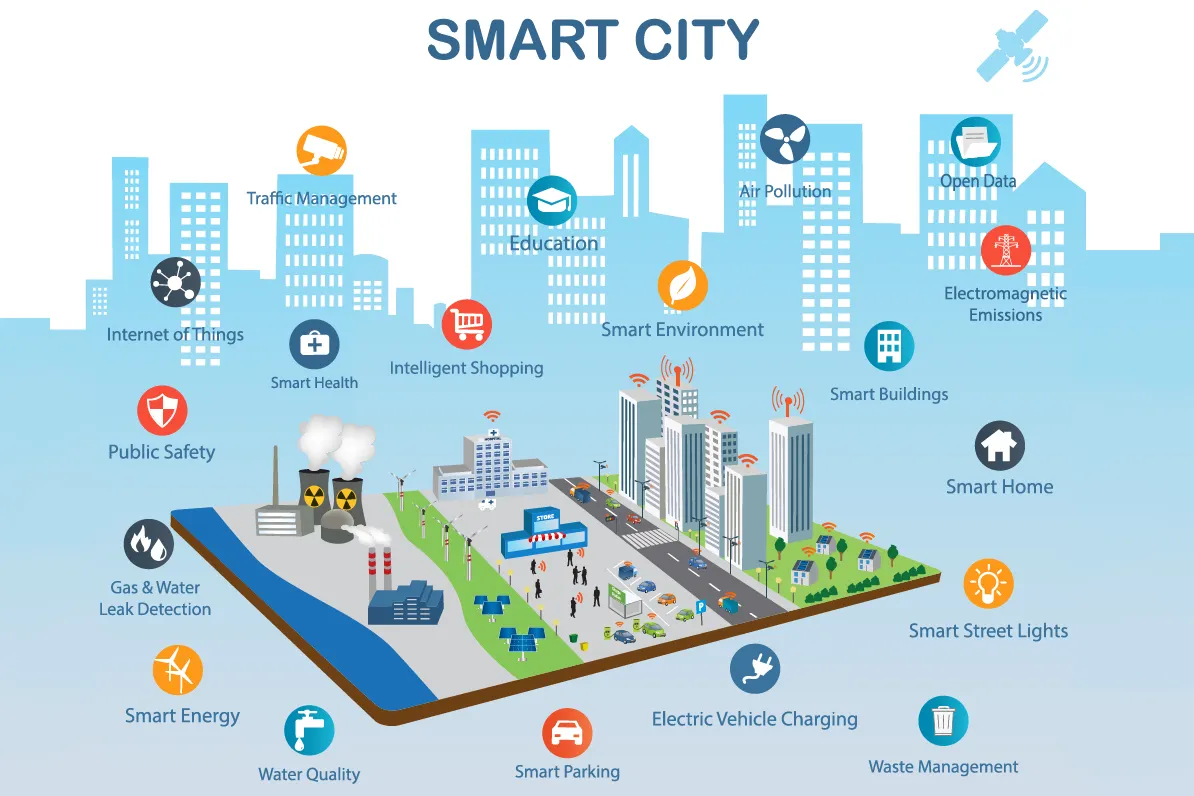
\includegraphics[width=0.85\textwidth]
  {smartcity_dimensions}
\caption{Les composantes d'une ville intelligente}
\label{fig:smartcity_dimensions}
\end{figure}

Ce n'est pas un concept abstrait. À Agadir,
la transformation en ville intelligente est
inscrite dans un programme officiel depuis 2022,
avec des axes concrets qui touchent directement
à la mobilité urbaine.

\subsection{Les six dimensions d'une smart city}

La littérature identifie six dimensions
complémentaires qui structurent le concept
de ville intelligente~\cite{hazarika2024}.
La première est la \textbf{Smart Mobility} :
systèmes de transport connectés, régulation
du trafic en temps réel, réduction de la
congestion. La deuxième est le \textbf{Smart
Environment} : gestion durable des ressources,
réduction des émissions. Viennent ensuite la
\textbf{Smart Economy}, la \textbf{Smart
Governance}, le \textbf{Smart Living} et
les \textbf{Smart People} — qui désigne
l'implication active des habitants dans
les transformations urbaines.

Notre travail s'inscrit directement dans
la dimension Smart Mobility, qui conditionne
la fluidité urbaine, la qualité de l'air
et la sécurité des usagers.

\subsection{Le Maroc et l'initiative Smart City
            Agadir}

Le Maroc s'est engagé dans une stratégie
nationale de transformation numérique qui
touche plusieurs secteurs : mobilité,
sécurité urbaine, énergie et services
numériques~\cite{elalaoui2025}. Agadir a
lancé en 2022 son programme officiel de
transformation, structuré autour de douze
axes dans le cadre du Plan d'Action Communal
2022--2027.

\begin{figure}[H]
\centering
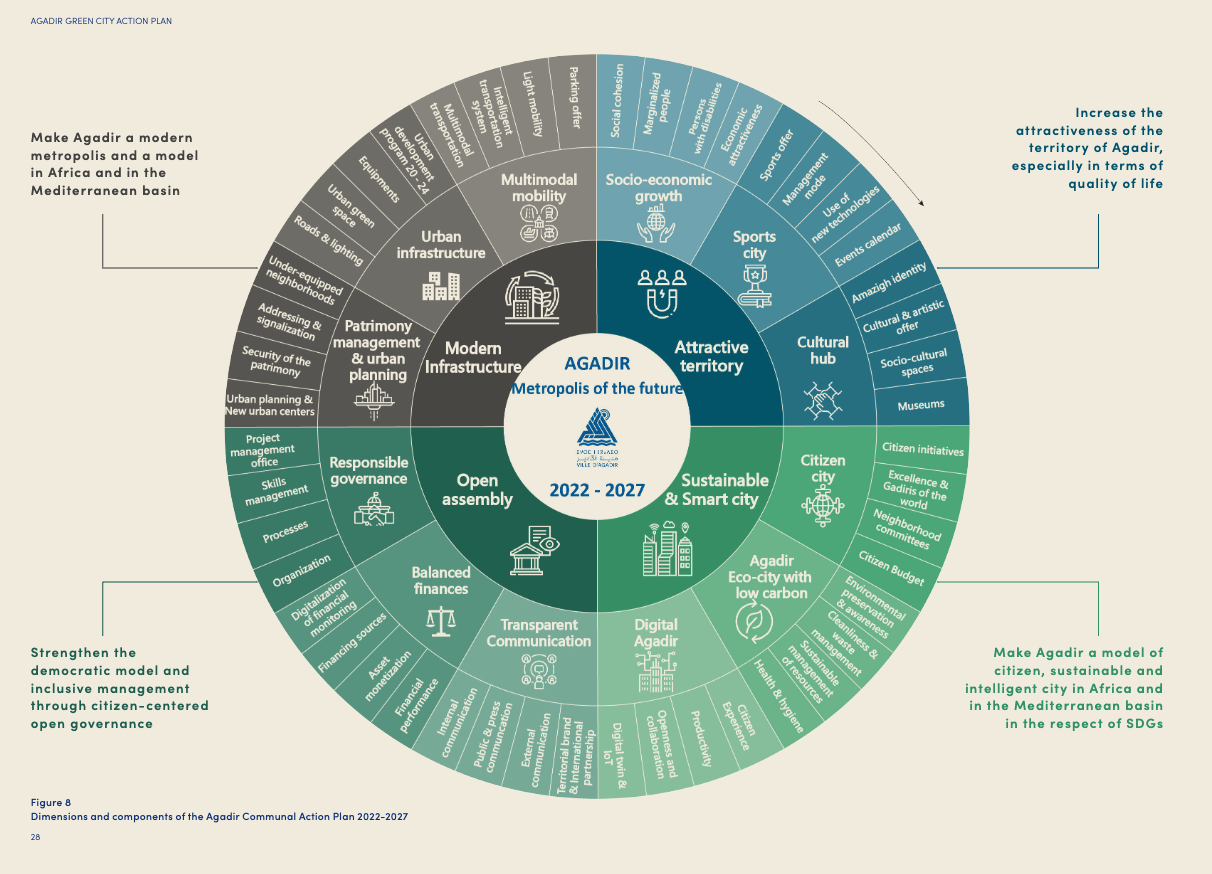
\includegraphics[width=0.85\textwidth]
  {agadir_smartcity}
\caption{Axes du Plan d'Action Communal
         d'Agadir 2022--2027
\textit{(Source : Agadir Green City
         Action Plan, Ville d'Agadir, 2022)}}
\label{fig:agadir_plan}
\end{figure}

Une étude menée auprès de 98 jeunes résidents
d'Agadir montre que la majorité soutient cette
transformation, avec une adhésion fortement
corrélée au niveau d'éducation et à la maîtrise
du numérique~\cite{elalaoui2025}. C'est dans
ce contexte favorable que s'inscrit le système
développé dans ce mémoire.

\subsection{La gestion du trafic comme
            composante centrale}

La mobilité est l'une des premières dimensions
visibles d'une ville intelligente, parce qu'elle
affecte directement la vie quotidienne des
habitants. Les feux à cycles fixes — encore
majoritaires dans les villes marocaines —
fonctionnent selon des durées prédéfinies,
sans tenir compte de ce qui se passe réellement
à l'intersection. Résultat : des files d'attente
inutiles quand une voie est vide, et des
blocages quand le trafic dépasse les hypothèses
de dimensionnement du cycle.

\begin{table}[H]
\centering
\caption{Feux à cycles fixes vs système
         adaptatif intelligent}
\begin{tabularx}{\textwidth}{Xcc}
\toprule
\textbf{Critère} &
\textbf{Feux fixes} &
\textbf{Système adaptatif} \\
\midrule
Temps d'attente moyen &
Élevé & Réduit \\
Adaptation au trafic réel &
Non & Oui \\
Priorité véhicules urgence &
Non & Oui \\
Gestion heures de pointe &
Inefficace & Optimisée \\
Détection piétons &
Non & Oui \\
Conformité Loi 09-08 &
Non applicable & Intégrée \\
\bottomrule
\end{tabularx}
\label{tab:feux_comparaison}
\end{table}

Hazarika et al. (2024) confirment qu'un système
basé sur la détection YOLO permet de réduire
significativement les temps d'attente aux
intersections~\cite{hazarika2024}. La
Figure~\ref{fig:traffic_ai} illustre un exemple
de détection et comptage par zones — principe
au cœur de notre approche.

\begin{figure}[H]
\centering
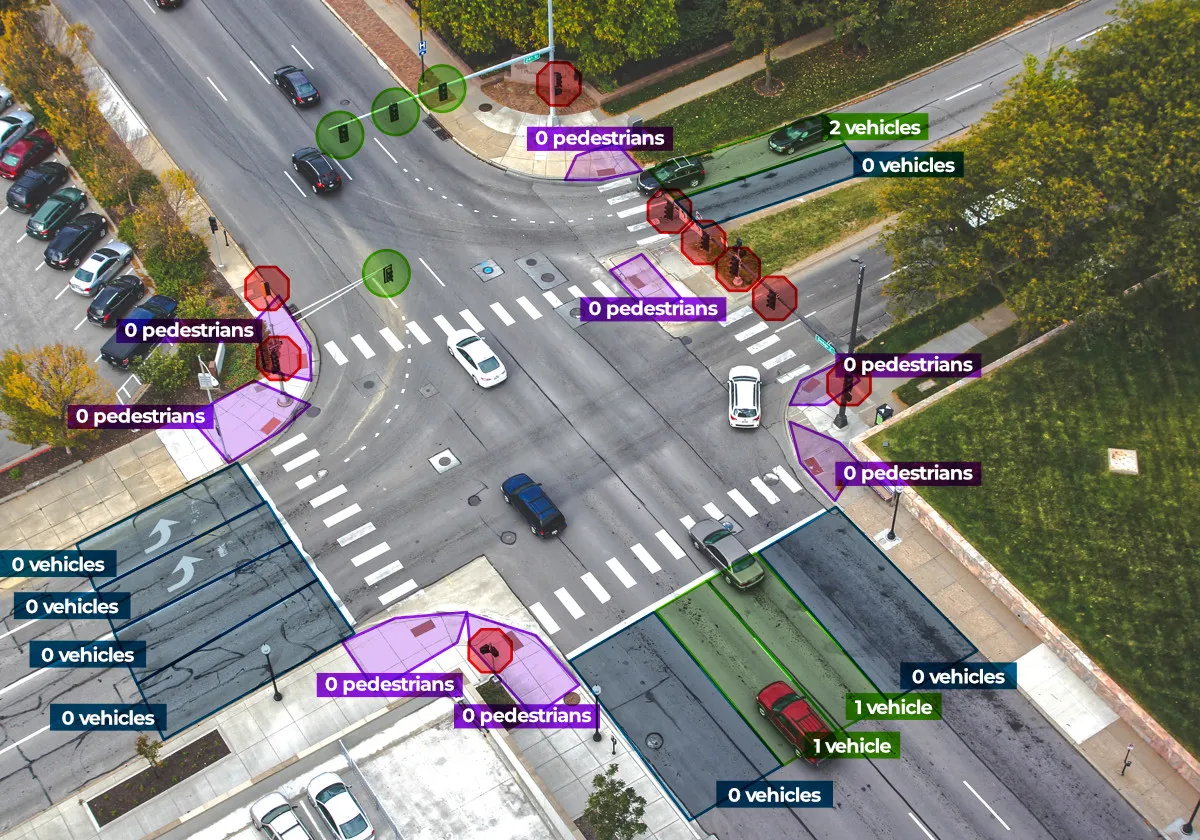
\includegraphics[width=0.90\textwidth]
  {traffic_intersection_ai}
\caption{Détection et comptage des véhicules
         et piétons par zones à une intersection
\textit{(Source : Parquery, 2024)}}
\label{fig:traffic_ai}
\end{figure}

\section{Détection d'objets en temps réel}

\subsection{Définition et enjeux}

La détection d'objets consiste à répondre
simultanément à deux questions sur une image :
\textit{qu'est-ce que c'est ?} et
\textit{où est-ce ?}~\cite{ramos2025}.
C'est différent de la simple classification,
qui identifie sans localiser.

Dans notre cas, on a besoin des deux en même
temps : identifier si un objet est une voiture,
un piéton ou une ambulance, et savoir dans
quelle zone de l'intersection il se trouve
pour alimenter la décision MDP. Et tout ça
en temps réel, sur un CPU ARM sans GPU dédié.

\subsection{Approches one-stage et two-stage}

Il existe deux grandes familles d'algorithmes
de détection. Les approches \textbf{two-stage}
— comme Faster R-CNN — fonctionnent en deux
étapes : d'abord générer des régions candidates,
puis les classifier. Cette double passe donne
une bonne précision, mais au prix d'une latence
incompatible avec le temps réel~\cite{ramos2025}.

\begin{figure}[H]
\centering
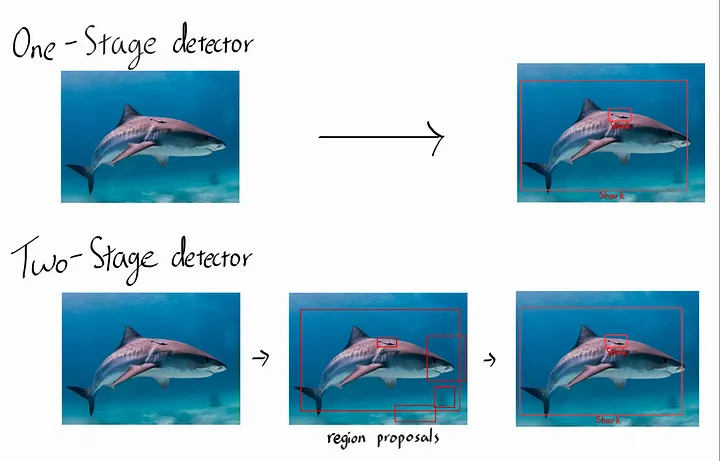
\includegraphics[width=0.95\textwidth]{1vs2_stages}
\caption{Comparaison des approches one-stage
         et two-stage
\textit{(Source : Sharkyun, Medium, 2024)}}
\label{fig:detection_approaches}
\end{figure}

Les approches \textbf{one-stage} — YOLO, SSD,
RetinaNet — font tout en un seul passage :
localisation et classification simultanément.
C'est plus rapide, avec une légère concession
sur la précision. C'est la seule option viable
pour un déploiement sur Raspberry Pi 5.

\begin{figure}[H]
\centering
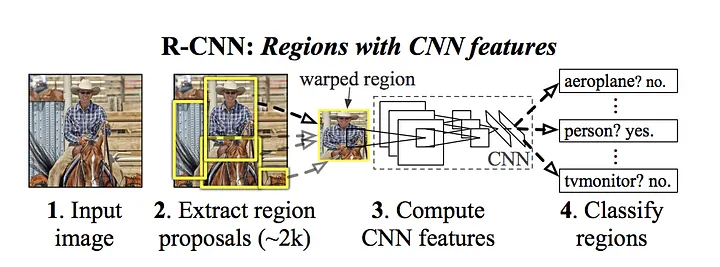
\includegraphics[width=0.92\textwidth]
  {2stagedetection}
\caption{Fonctionnement d'une approche two-stage
\textit{(Source : Sharkyun, Medium, 2024)}}
\label{fig:two_stage_detection}
\end{figure}

\begin{figure}[H]
\centering
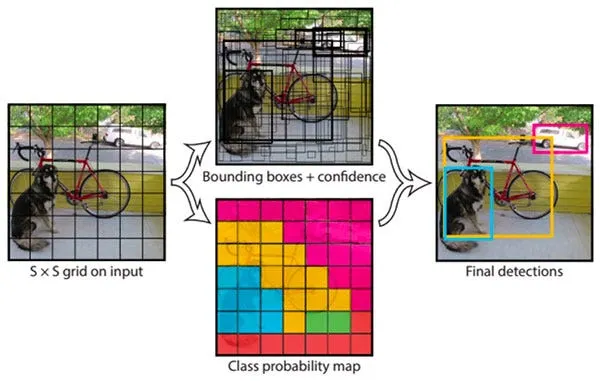
\includegraphics[width=0.92\textwidth]
  {1stagedetection}
\caption{Fonctionnement d'une approche one-stage
\textit{(Source : Sharkyun, Medium, 2024)}}
\label{fig:one_stage_detection}
\end{figure}

\begin{table}[H]
\centering
\caption{Comparaison one-stage et two-stage}
\begin{tabularx}{\textwidth}{Xcc}
\toprule
\textbf{Critère} &
\textbf{Two-Stage} &
\textbf{One-Stage} \\
\midrule
Vitesse d'inférence &
Faible & \textbf{Élevée} \\
Précision (mAP) &
\textbf{Élevée} & Bonne \\
Temps réel sur CPU ARM &
Impossible & \textbf{Oui} \\
Déploiement embarqué &
Non & \textbf{Oui} \\
Exemples &
Faster R-CNN & \textbf{YOLO, SSD} \\
\bottomrule
\end{tabularx}
\label{tab:one_two_stage}
\end{table}

\subsection{Métriques d'évaluation}

Plusieurs métriques standardisées sont utilisées
pour évaluer les modèles de détection. On les
retrouve tout au long de ce mémoire, il est
utile de les définir ici.

\subsubsection{Intersection over Union (IoU)}

L'IoU mesure le chevauchement entre la boîte
prédite $\hat{B}$ et la boîte réelle $B$ :

\begin{equation}
\text{IoU} = \frac{|\hat{B} \cap B|}
             {|\hat{B} \cup B|}
\label{eq:iou}
\end{equation}

Une détection est considérée correcte
si $\text{IoU} \geq 0.5$.

\subsubsection{Précision et Rappel}

La \textbf{précision} mesure combien de
détections sont justes parmi toutes celles
produites :

\begin{equation}
\text{Précision} = \frac{VP}{VP + FP}
\label{eq:precision}
\end{equation}

Le \textbf{rappel} mesure combien d'objets
réels ont été détectés :

\begin{equation}
\text{Rappel} = \frac{VP}{VP + FN}
\label{eq:recall}
\end{equation}

Ces deux métriques sont souvent en tension :
augmenter le rappel tend à réduire la
précision, et inversement.

\subsubsection{Mean Average Precision (mAP)}

La mAP est la métrique de référence pour
comparer les modèles de détection. Elle calcule
la moyenne des précisions moyennes sur toutes
les classes $C$ :

\begin{equation}
\text{mAP} = \frac{1}{C} \sum_{c=1}^{C} AP_c
\label{eq:map}
\end{equation}

Dans ce travail, on utilise la \textbf{mAP@50}
(IoU $\geq$ 0.5) et la \textbf{mAP@50-95}
(moyenne sur IoU de 0.5 à 0.95, pas de 0.05).
La mAP@50-95 est plus stricte et pénalise
les localisations imprécises.

\subsubsection{Non-Maximum Suppression (NMS)}

Le NMS est un post-traitement qui élimine
les détections redondantes sur le même objet.
Pour chaque classe, il garde uniquement la
boîte avec la confiance la plus haute parmi
celles qui se chevauchent trop :

\begin{equation}
\hat{B}^* = \arg\max_{\hat{B}}
\text{conf}(\hat{B})\
\text{s.t.}\
\text{IoU}(\hat{B}, \hat{B}') < \theta_{NMS}
\label{eq:nms}
\end{equation}

\begin{definitionbox}{NMS-Free dans YOLO26n}
YOLO26n supprime l'étape NMS grâce à un
mécanisme d'assignation One-to-One introduit
dans YOLOv10. Sur CPU ARM, supprimer ce
post-traitement réduit directement la latence
d'inférence — un avantage concret pour
le déploiement sur Raspberry Pi 5~\cite{sapkota2025}.
\end{definitionbox}

\section{Architecture YOLO : évolution et
         innovations}

\subsection{Principe fondamental}

YOLO (\textit{You Only Look Once}) a été
introduit par Redmon et al. en 2015 avec
une idée simple : au lieu de parcourir
l'image en plusieurs étapes, on la traite
en une seule passe~\cite{ramos2025}.

Le réseau divise l'image en une grille
de $S \times S$ cellules. Pour chaque
cellule, il prédit simultanément les boîtes
englobantes et les probabilités de classe.
La prédiction finale pour chaque boîte est :

\begin{equation}
\text{Score} = P(\text{classe}_i | \text{objet})
\times \text{IoU}_{pred}^{truth}
\label{eq:yolo_score}
\end{equation}

\begin{figure}[H]
\centering
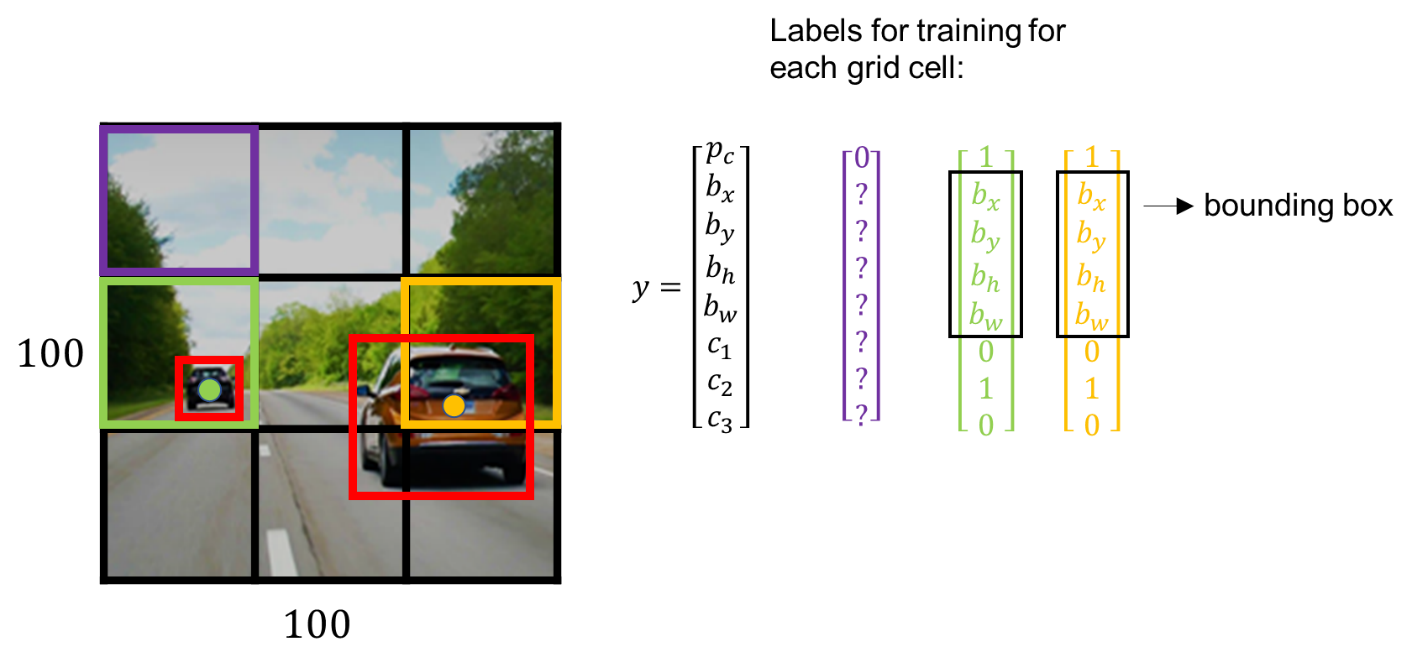
\includegraphics[width=0.88\textwidth]{yoloxyz}
\caption{Détection YOLO : grille et prédiction
         des boîtes englobantes
\textit{(Source : Blent.ai, 2024)}}
\label{fig:yolo_grid}
\end{figure}

\subsection{Architecture générale}

Toutes les versions modernes de YOLO partagent
la même structure en trois blocs :

\begin{figure}[H]
\centering
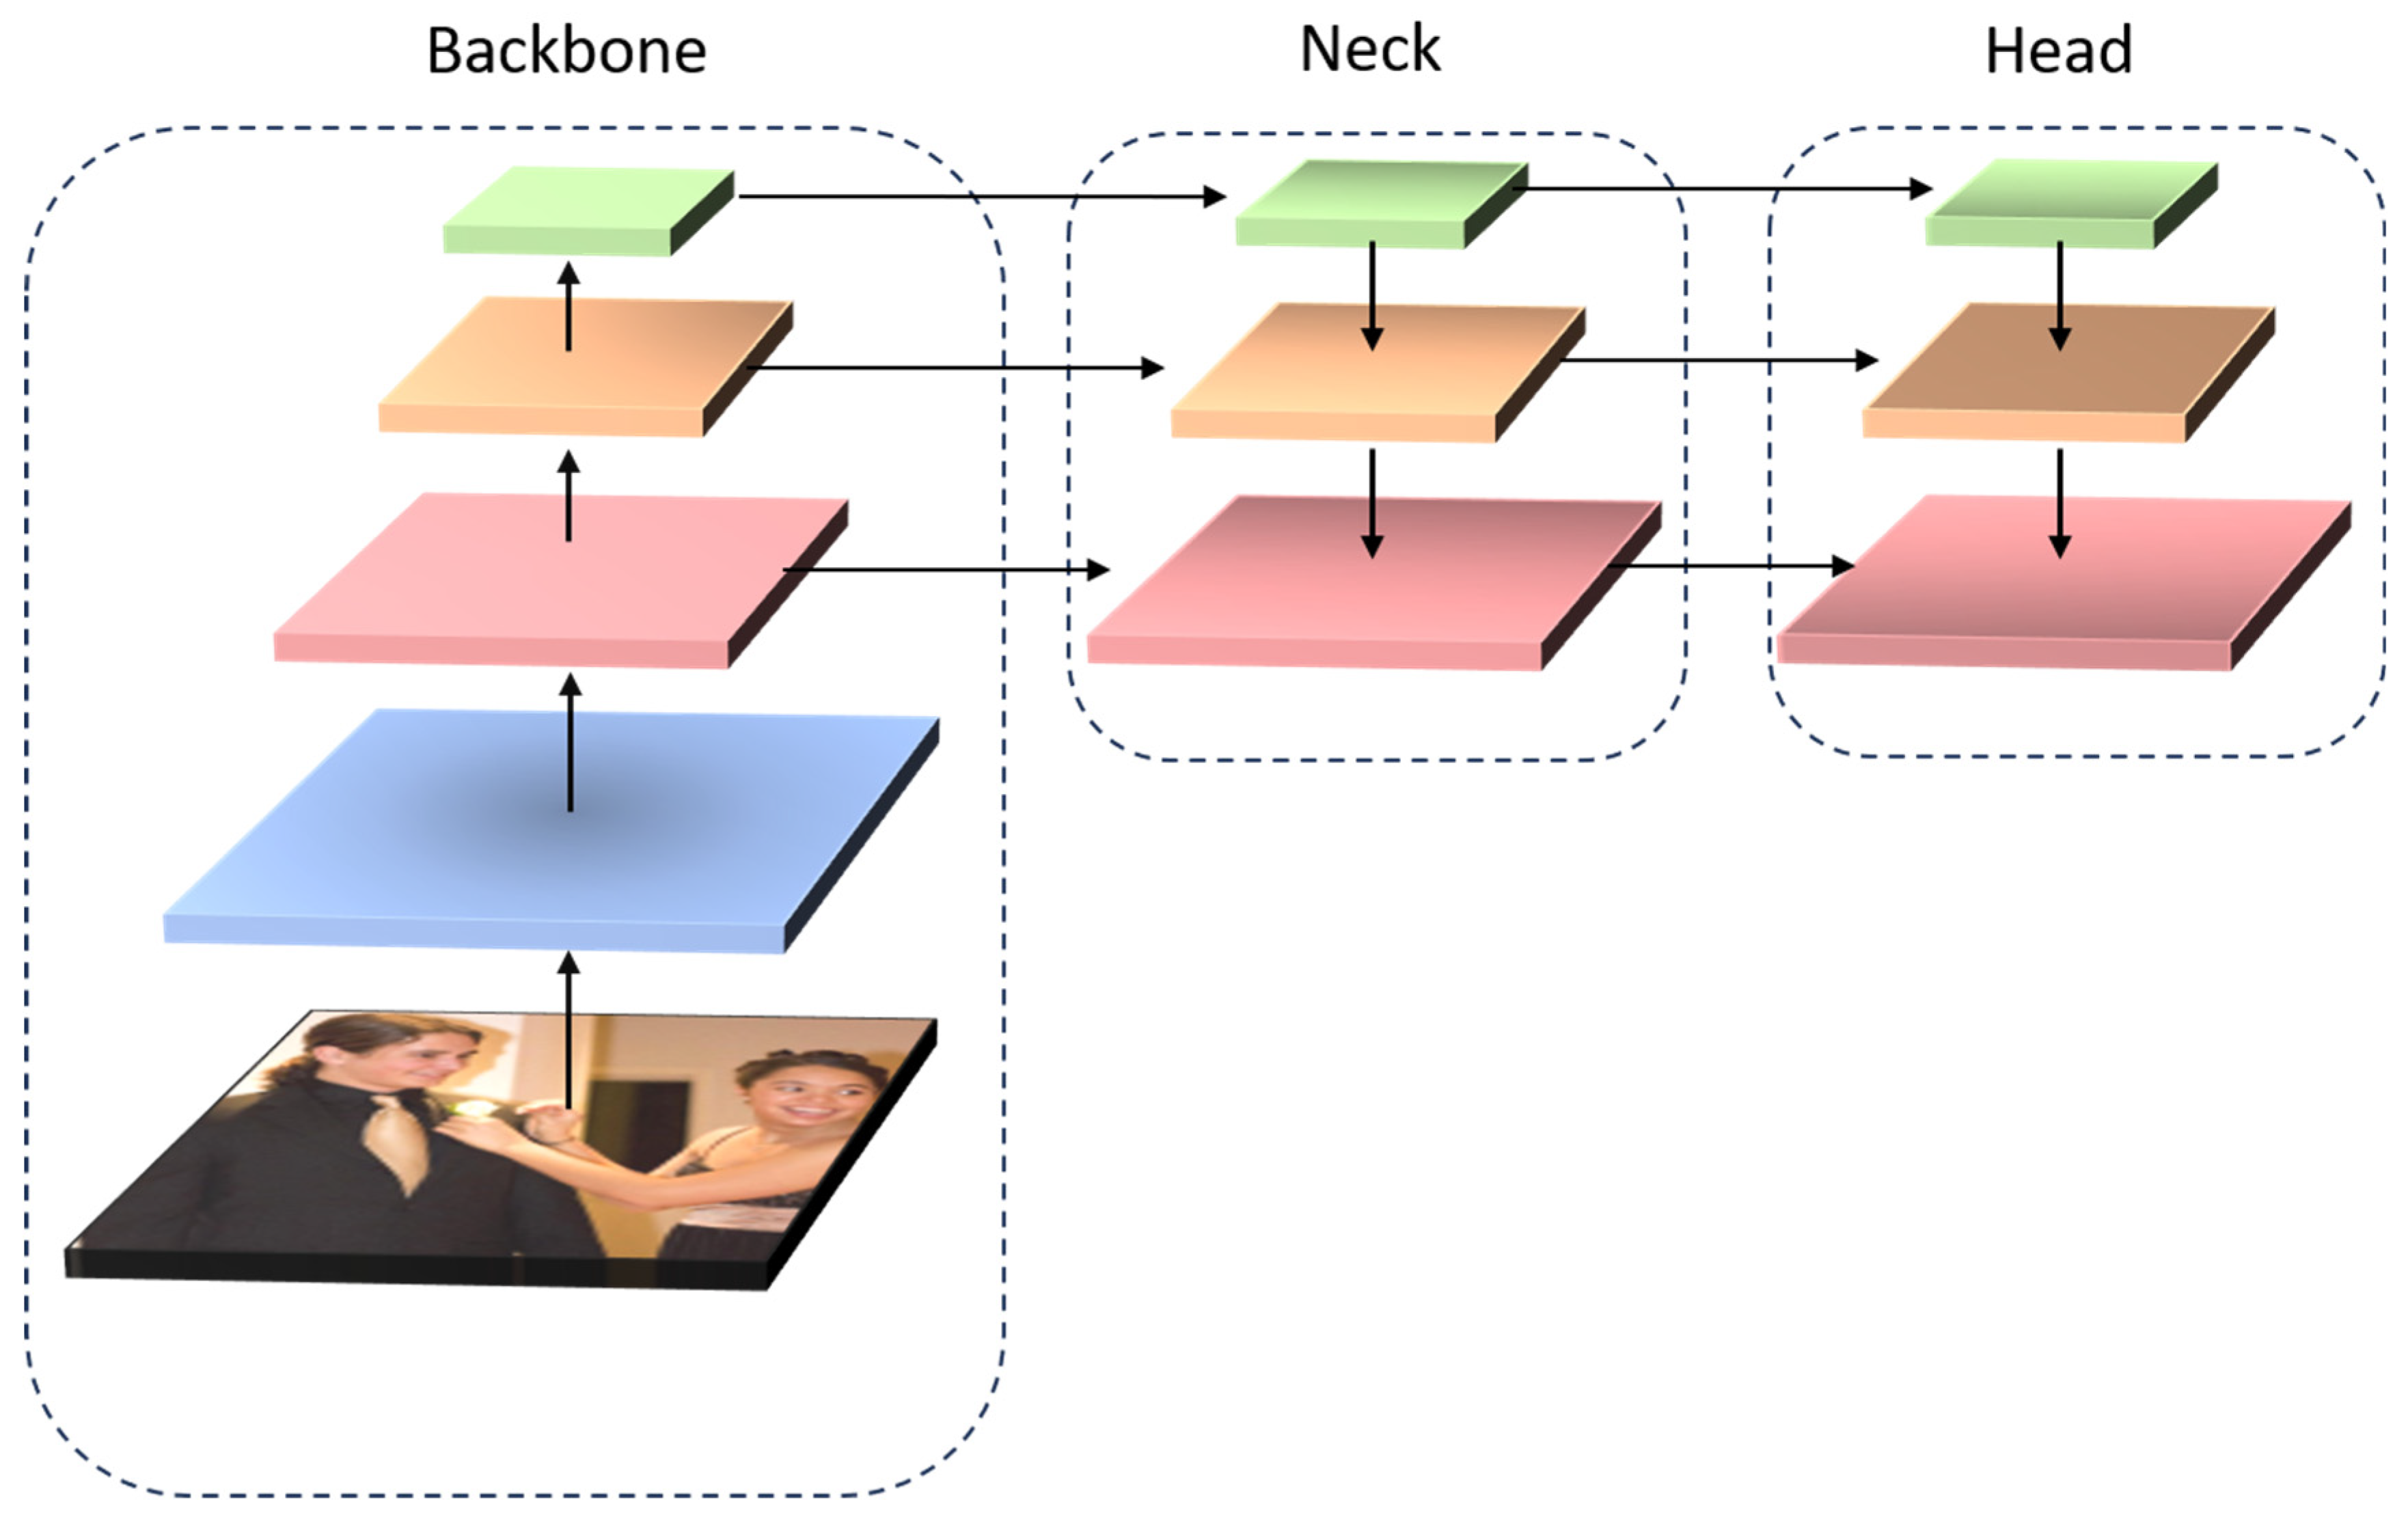
\includegraphics[width=0.95\textwidth]
  {yoloarchitecture}
\caption{Architecture générale d'un modèle
         YOLO moderne
\textit{(Source : MDPI Electronics, 2025)}}
\label{fig:yolo_architecture}
\end{figure}

Le \textbf{Backbone} extrait les
caractéristiques visuelles de l'image à
différents niveaux d'abstraction. Dans
YOLO26n, il utilise les blocs C3k2 et C2PSA.
Le \textbf{Neck} fusionne ces caractéristiques
à différentes résolutions via FPN et PAN,
ce qui permet de détecter des objets de
tailles variées — petits piétons comme
grands camions. La \textbf{Head} produit
les prédictions finales : coordonnées,
scores de confiance et classes. Les
architectures récentes utilisent une
\textit{Decoupled Head} qui sépare les
tâches de classification et de régression
pour de meilleures performances.

\subsection{Évolution de YOLOv1 à YOLO26}

En dix ans, la famille YOLO a évolué
considérablement, chaque version apportant
des innovations architecturales mesurables
sur des benchmarks standardisés~\cite{ramos2025}.

\begin{table}[H]
\centering
\caption{Évolution des principales versions
         YOLO (2015--2025)}
\begin{tabularx}{\textwidth}{llX}
\toprule
\textbf{Version} &
\textbf{Année} &
\textbf{Innovation principale} \\
\midrule
YOLOv1 & 2015 &
Détection unifiée en une passe,
grille $7\times7$ \\
YOLOv2 & 2016 &
Anchor boxes, entraînement multi-échelle \\
YOLOv3 & 2018 &
Détection à trois niveaux de résolution \\
YOLOv4 & 2020 &
CSP, augmentation Mosaic, CIoU Loss \\
YOLOv5 & 2020 &
Migration PyTorch, variantes
nano/small/medium/large \\
YOLOv7 & 2022 &
E-ELAN, meilleur compromis
vitesse/précision \\
YOLOv8 & 2023 &
Anchor-free, Decoupled Head,
architecture Ultralytics unifiée \\
YOLOv9 & 2024 &
GELAN, Programmable Gradient
Information \\
YOLOv10 & 2024 &
Suppression du NMS, assignation
One-to-One \\
YOLOv11 & 2024 &
C3k2, PSA, amélioration backbone \\
\rowcolor{PrimaryBlue!15}
\textbf{YOLO26} & \textbf{2025} &
\textbf{ProgLoss, STAL, MuSGD,
NMS-Free natif, optimisé edge} \\
\bottomrule
\end{tabularx}
\label{tab:yolo_evolution}
\end{table}

\subsection{Pourquoi YOLO26n a été retenu}

Lors du benchmark, YOLOv8n et YOLOv11n
affichaient une précision parfois proche
ou légèrement meilleure que YOLO26n. Le
choix n'était donc pas évident si on
regardait uniquement les métriques GPU.

C'est le benchmark Raspberry Pi 5 qui a
tranché. Sur CPU ARM, la différence devient
visible :

\begin{table}[H]
\centering
\caption{Comparaison embarquée des variantes
         nano sur Raspberry Pi 5}
\begin{tabularx}{\textwidth}{lcccc}
\toprule
\textbf{Modèle} &
\textbf{Format} &
\textbf{FPS Pi 5} &
\textbf{mAP50} &
\textbf{Params} \\
\midrule
YOLOv8n  & FP32 & 5.3 & 69.8\% & 3.0M \\
YOLOv11n & FP32 & 5.9 & 69.2\% & 2.6M \\
\rowcolor{PrimaryBlue!15}
\textbf{YOLO26n} &
\textbf{FP32} & \textbf{7.6} &
65.6\% & \textbf{2.4M} \\
\bottomrule
\end{tabularx}
\label{tab:yolo_benchmark}
\end{table}

YOLO26n est retenu pour trois raisons
concrètes. Premièrement, il atteint 7.6 FPS
réels sur le Pi 5 — la marge la plus
importante au-dessus du seuil minimal de
5 FPS, ce qui laisse des ressources CPU
disponibles pour les autres modules du
pipeline. Deuxièmement, son architecture
NMS-Free réduit directement la latence sur
CPU ARM, là où les autres modèles paient
encore le coût du post-traitement.
Troisièmement, avec 2.4M de paramètres et
environ 9.8 MB en ONNX FP32, son empreinte
mémoire est la plus faible des trois.

YOLO26n intègre aussi trois innovations
spécifiques qui l'ont rendu attractif pour
ce projet~\cite{sapkota2025} : ProgLoss
pour une convergence plus stable à
l'entraînement, STAL (\textit{Small
Target-Aware Learning}) pour améliorer la
détection des petits objets — piétons et
motos notamment —, et MuSGD, un optimiseur
hybride inspiré des grands modèles de
langage qui accélère la convergence jusqu'à
47\% par rapport aux optimiseurs classiques.

\section{Edge AI et déploiement embarqué}

\subsection{Définition et positionnement}

L'Edge AI consiste à exécuter les modèles
d'intelligence artificielle directement
sur le dispositif qui collecte les données,
sans envoyer quoi que ce soit vers un
serveur distant. Dans notre architecture,
c'est à la fois un choix technique et une
nécessité juridique~\cite{ficili2025}.

\begin{figure}[H]
\centering
\resizebox{0.90\textwidth}{!}{%
\begin{tikzpicture}[
  font=\footnotesize,
  stack/.style={
    draw, rounded corners=7pt,
    align=center, minimum width=4.2cm,
    minimum height=0.88cm, very thick
  },
  cloud/.style={stack,
    draw=red!65, fill=red!8},
  edge/.style={stack,
    draw=AccentGreen, fill=AccentGreen!8},
  title/.style={
    font=\bfseries\small, align=center},
  choice/.style={
    draw=PrimaryBlue, fill=PrimaryBlue!6,
    rounded corners=6pt, align=center,
    text width=9.4cm,
    minimum height=0.95cm,
    font=\scriptsize\bfseries
  },
  note/.style={
    draw=DarkGray!45, fill=white,
    rounded corners=4pt, align=center,
    font=\scriptsize, text width=4.3cm
  },
  arrow/.style={
    -{Latex[length=3mm]},
    line width=1pt}
]

\node[title, color=red!70] at (0,0)
  {Architecture Cloud};
\node[cloud] (c1) at (0,-1.00) {Caméra};
\node[cloud] (c2) at (0,-2.25)
  {Transmission réseau};
\node[cloud] (c3) at (0,-3.50)
  {Serveur distant};
\node[note, draw=red!45] at (0,-4.85)
  {Images brutes transmises hors de
   l'intersection. Risque juridique réel.};

\node[title, color=AccentGreen] at (7.2,0)
  {Architecture Edge AI retenue};
\node[edge] (e1) at (7.2,-1.00) {Caméra};
\node[edge, draw=PrimaryBlue,
      fill=PrimaryBlue!8] (e2) at (7.2,-2.25)
  {Raspberry Pi 5\\YOLO26n FP32};
\node[edge] (e3) at (7.2,-3.50)
  {Décision locale};
\node[note, draw=AccentGreen!55] at (7.2,-4.85)
  {Traitement local, aucune donnée
   personnelle ne quitte l'intersection.};

\draw[arrow, red!65] (c1) -- (c2);
\draw[arrow, red!65] (c2) -- (c3);
\draw[arrow, AccentGreen] (e1) -- (e2);
\draw[arrow, AccentGreen] (e2) -- (e3);

\node[choice] at (3.6,-6.25)
  {Choix retenu : traitement local,
   latence faible, conformité Loi 09-08.};

\end{tikzpicture}}
\caption{Architecture Cloud vs Edge AI
         pour la gestion du trafic}
\label{fig:cloud_vs_edge}
\end{figure}

Un système cloud transmet les flux vidéo
vers des serveurs distants — ce qui revient
à envoyer en continu des images contenant
des visages et des plaques d'immatriculation
hors de l'intersection. C'est exactement
ce que la Loi 09-08 encadre strictement.
Le traitement local sur le Pi 5 règle ce
problème à la racine.

\subsection{Défis spécifiques du Raspberry Pi 5}

Déployer un pipeline de vision par ordinateur
sur CPU ARM soulève des contraintes absentes
des environnements GPU d'entraînement~\cite{wang2025}.

Le processeur ARM Cortex-A76 n'a pas d'unité
de calcul tensoriel : toute l'inférence repose
sur le CPU. La RAM de 8 Go est partagée entre
le système, le modèle et le pipeline vidéo.
La dissipation thermique est limitée — une
charge CPU soutenue peut déclencher le
\textit{thermal throttling} et réduire les
performances. Et enfin, la gestion du trafic
exige au minimum 5 FPS pour que les décisions
restent cohérentes avec l'évolution réelle
de l'intersection.

\subsection{Optimisations retenues}

\subsubsection{Variante nano uniquement}

Le benchmark a confirmé empiriquement que
les variantes \textit{small} ne passent pas
la barre des 3 FPS sur Raspberry Pi 5, quel
que soit le format d'export. Les variantes
nano sont les seules compatibles avec le
temps réel sur CPU ARM~\cite{wang2025}.

\subsubsection{Format FP32 retenu, INT8 écarté}

La quantification INT8 réduit la taille du
modèle, mais elle n'apporte pas de gain FPS
systématique sur Raspberry Pi 5 et introduit
une confusion plus marquée entre les classes
visuellement proches — notamment car, bus et
truck. Le format FP16 est incompatible avec
le CPU ARM Cortex-A76 : sans Tensor Cores,
les opérations FP16 sont émulées en logiciel
et ralentissent l'inférence. Le format FP32
est donc retenu.

\begin{table}[H]
\centering
\caption{Formats de précision sur
         Raspberry Pi 5 — modèle de base}
\begin{tabularx}{\textwidth}{lccXl}
\toprule
\textbf{Format} &
\textbf{FPS} &
\textbf{Latence} &
\textbf{Observation} &
\textbf{Décision} \\
\midrule
FP32 & 3.7 & 178ms &
Référence stable &
Retenu \\
FP16 & — & — &
Incompatible CPU ARM &
Écarté \\
INT8 & 5.0 & 193ms &
Confusion car/bus/truck &
Écarté \\
\bottomrule
\end{tabularx}
\label{tab:formats}
\end{table}

\subsubsection{Export ONNX}

Le modèle PyTorch natif est optimisé pour
GPU et peu efficace sur CPU ARM. L'export
au format ONNX (\textit{Open Neural Network
Exchange}) permet d'utiliser ONNX Runtime
avec le fournisseur \texttt{CPUExecutionProvider},
conçu pour maximiser l'inférence sur
processeur~\cite{wang2025} :

\begin{equation}
\texttt{best.pt}
\xrightarrow{\text{export}}
\texttt{yolo26n.onnx}
\xrightarrow{\text{ONNX Runtime}}
\text{Inférence Pi 5}
\label{eq:onnx}
\end{equation}

\section{Protection des données personnelles}

\subsection{Cadre légal marocain — Loi 09-08}

La Loi n°09-08 du 18 février 2009 est le texte
de référence au Maroc pour la protection des
données personnelles. Elle a institué la
Commission Nationale de contrôle de la
protection des Données à caractère Personnel
(CNDP), dont la mission est de vérifier que
tout traitement de données est licite et ne
porte pas atteinte aux droits fondamentaux
des citoyens~\cite{elalaoui2025}. Le texte
complet est disponible sur le site officiel
de la CNDP.

\begin{figure}[H]
\centering
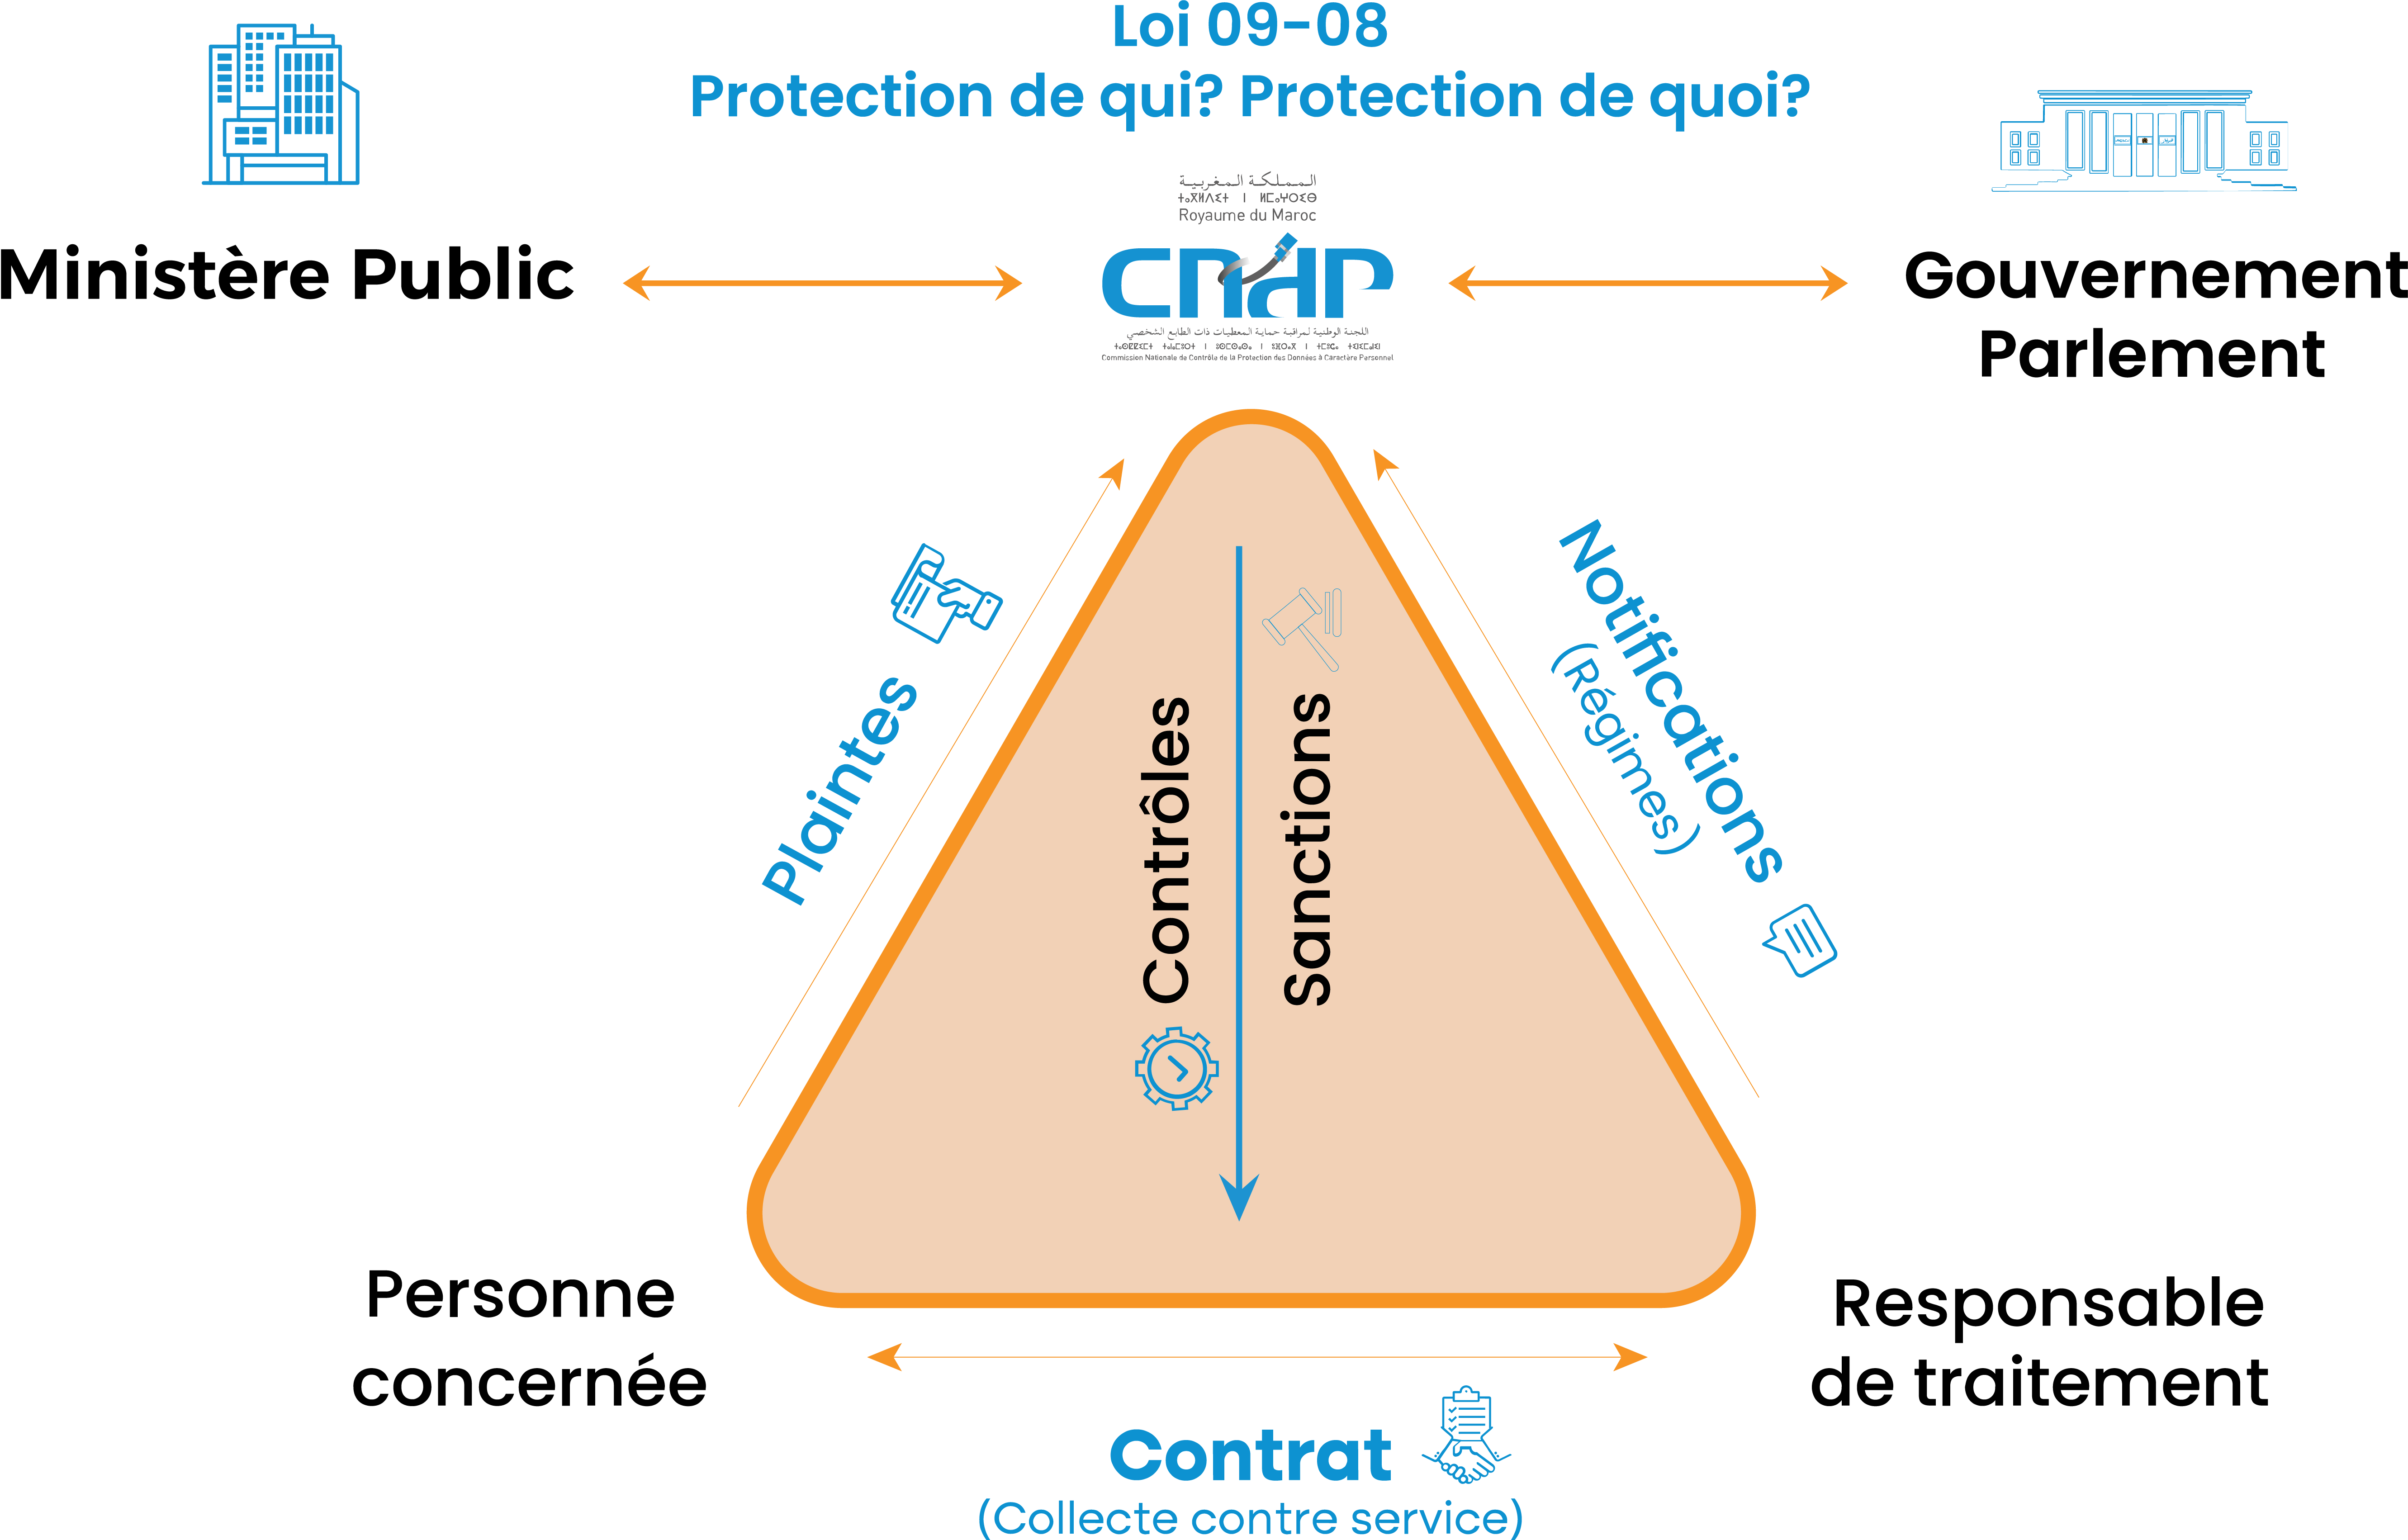
\includegraphics[width=0.55\textwidth]{cndp}
\caption{Logo de la CNDP, autorité marocaine
         de protection des données
\textit{(Source : cndp.ma, 2024)}}
\label{fig:cndp}
\end{figure}

La loi repose sur quatre principes fondamentaux.
La \textbf{finalité} : les données ne peuvent
être utilisées qu'aux fins déclarées.
La \textbf{proportionnalité} : on ne collecte
que ce qui est strictement nécessaire.
La \textbf{sécurité} : des mesures techniques
adaptées doivent protéger les données.
Et la \textbf{durée limitée} : on ne conserve
pas les données au-delà du nécessaire.

\subsection{Enjeux dans les systèmes de
            surveillance du trafic}

Une caméra installée à un carrefour ne filme
pas que des voitures. Elle capture aussi des
visages — donnée biométrique sensible —, des
plaques d'immatriculation qui permettent
d'identifier le propriétaire du véhicule,
et des patterns de déplacement qui révèlent
les habitudes de vie. Ce sont toutes des
données personnelles au sens de la Loi 09-08.

Des travaux récents montrent que même des
images partiellement anonymisées restent
vulnérables à des attaques de ré-identification
par des algorithmes d'IA avancés~\cite{razi2025}.
Flouter a posteriori ne suffit pas si les
données brutes ont déjà circulé dans le
système.

\begin{figure}[H]
\centering
\resizebox{0.92\textwidth}{!}{%
\begin{tikzpicture}[
  font=\small,
  cell/.style={
    draw, rounded corners=4pt,
    align=center, minimum width=4.05cm,
    minimum height=0.72cm,
    font=\scriptsize
  },
  risk/.style={cell,
    draw=red!60, fill=red!8},
  sol/.style={cell,
    draw=AccentGreen, fill=AccentGreen!8},
  head/.style={
    draw, rounded corners=5pt,
    align=center, minimum width=4.05cm,
    minimum height=0.72cm,
    font=\small\bfseries, text=white
  },
  arrow/.style={
    -{Latex[length=2.7mm]},
    line width=0.95pt, PrimaryBlue}
]

\node[head, fill=red!68] at (0,0) {Risque};
\node[head, fill=PrimaryBlue] at (5.0,0)
  {Mesure technique};
\node[head, fill=AccentGreen!80!black]
  at (10.0,0) {Effet obtenu};

\node[risk] (r1) at (0,-0.95)
  {Identification directe};
\node[sol]  (m1) at (5.0,-0.95)
  {Floutage gaussien\\des personnes};
\node[sol]  (e1) at (10.0,-0.95)
  {Visages non exploitables};

\node[risk] (r2) at (0,-1.85)
  {Suivi des déplacements};
\node[sol]  (m2) at (5.0,-1.85)
  {Tracking après anonymisation};
\node[sol]  (e2) at (10.0,-1.85)
  {Identité non conservée};

\node[risk] (r3) at (0,-2.75)
  {Fuite de données};
\node[sol]  (m3) at (5.0,-2.75)
  {Traitement local Edge AI};
\node[sol]  (e3) at (10.0,-2.75)
  {Aucun envoi Cloud};

\node[risk] (r4) at (0,-3.65)
  {Non-conformité Loi 09-08};
\node[sol]  (m4) at (5.0,-3.65)
  {Anonymisation by design};
\node[sol]  (e4) at (10.0,-3.65)
  {Privacy-by-Design};

\foreach \r/\m/\e in
  {r1/m1/e1,r2/m2/e2,r3/m3/e3,r4/m4/e4}{
  \draw[arrow] (\r.east) -- (\m.west);
  \draw[arrow] (\m.east) -- (\e.west);
}

\node[
  draw=AccentOrange, fill=AccentOrange!7,
  rounded corners=5pt, align=center,
  font=\scriptsize, text width=9.6cm
] at (5.0,-4.65)
{Principe retenu : anonymiser avant toute
visualisation ou transmission, et limiter
le système aux statistiques nécessaires
à la décision de trafic.};
\end{tikzpicture}}
\caption{Risques de confidentialité et
         mesures adoptées dans notre système}
\label{fig:privacy_risks}
\end{figure}

\subsection{Techniques d'anonymisation}

Jeremiah et al. (2024) recensent plusieurs
techniques applicables aux flux vidéo de
surveillance~\cite{jeremiah2024}. Le floutage
gaussien est le plus rapide et le plus
compatible avec un déploiement edge. La
pixelisation est rapide aussi, mais reste
réversible par des algorithmes de
super-résolution. Les approches par
silhouette perdent trop d'information visuelle.
Les méthodes GAN sont trop lourdes pour un
Pi 5. La confidentialité différentielle est
complexe à calibrer en production.

\begin{table}[H]
\centering
\caption{Comparaison des techniques
         d'anonymisation vidéo}
\begin{tabularx}{\textwidth}{lllXl}
\toprule
\textbf{Technique} &
\textbf{Vitesse} &
\textbf{Edge} &
\textbf{Limite principale} &
\textbf{Retenu} \\
\midrule
Floutage gaussien &
Rapide & Oui &
Partiellement réversible &
\textbf{Oui} \\
Pixelisation &
Rapide & Oui &
Réversible par SR &
Non \\
Silhouette &
Moyen & Partiel &
Perte d'information &
Non \\
GAN anonymisation &
Lent & Non &
Trop lourd pour Pi 5 &
Non \\
Differential Privacy &
Variable & Partiel &
Complexe à calibrer &
Non \\
\bottomrule
\end{tabularx}
\label{tab:anon_techniques}
\end{table}

\subsection{Privacy-by-Design}

Le Privacy-by-Design est un principe
architectural qui dit que la protection des
données doit être intégrée dès la conception
du système, pas ajoutée en fin de pipeline.
Dans notre architecture, cela se traduit par
trois règles concrètes : le floutage est
appliqué immédiatement après la détection,
avant tout autre traitement ; aucune vidéo
n'est stockée ni transmise ; et l'intégralité
du pipeline s'exécute en local sur le Pi 5.

La limite de cette approche est connue et
documentée : le floutage gaussien reste
théoriquement vulnérable à des techniques
de super-résolution avancées~\cite{razi2025,
jeremiah2024}. Dans notre contexte — où
l'objectif est le comptage et non
l'identification — cette limite est
acceptable. Elle est néanmoins documentée
dans les limites du Chapitre 6.

\section{Décision adaptative des feux de
         circulation}

\subsection{Limites des systèmes à cycles fixes}

Un feu à cycle fixe ignore ce qui se passe
réellement à l'intersection. Il donne le vert
à une direction pendant 30 secondes même si
cette direction est vide, pendant qu'une
ambulance attend de l'autre côté. C'est le
problème concret que ce module cherche à
résoudre.

Li et al. (2025) quantifient les gains
possibles : une approche adaptative réduit
le temps d'attente moyen de 27,34\% par
rapport aux cycles fixes, avec des gains
atteignant 68,40\% dans les cas de trafic
fortement déséquilibré~\cite{li2025}.

\subsection{Formalisation MDP}

Un Processus de Décision Markovien (MDP)
est un cadre mathématique pour modéliser
la prise de décision séquentielle dans un
environnement dont l'état change en réponse
aux actions prises. Il est défini par le
quadruplet $(S, A, T, R)$~\cite{michailidis2025} :
l'espace d'états $S$, l'espace d'actions $A$,
la fonction de transition $T(s,a,s')$ et
la fonction de récompense $R(s,a)$.

\subsubsection{État $S$}

L'état de l'intersection est représenté par
un vecteur à six composantes :

\begin{equation}
s = (q_N,\ q_S,\ q_E,\ q_O,\ p,\ e)
\label{eq:state}
\end{equation}

où $q_N, q_S, q_E, q_O$ sont les densités
de véhicules dans les quatre directions,
$p$ est le nombre de piétons dans la zone
de passage, et $e$ indique la présence
d'un véhicule d'urgence ($e \in \{0,1\}$).

\subsubsection{Actions $A$}

Cinq phases de feux sont disponibles,
chacune associée à une durée variable
selon la densité détectée :

\begin{table}[H]
\centering
\caption{Phases et durées du module de
         décision}
\begin{tabularx}{\textwidth}{llXl}
\toprule
\textbf{Phase} &
\textbf{Feux verts} &
\textbf{Condition} &
\textbf{Durée} \\
\midrule
North-South & Nord + Sud &
Densité NS maximale & 15--45s \\
East-West   & Est + Ouest &
Densité EO maximale & 15--45s \\
Pedestrian  & Piétons &
Piétons + trafic faible & 30s \\
Emergency   & Tous rouges &
Véhicule urgence détecté & 45s \\
All-Red     & Aucun &
Aucun trafic & 15s \\
\bottomrule
\end{tabularx}
\label{tab:phases}
\end{table}

\subsubsection{Récompense $R$}

La récompense est l'opposé du temps
d'attente moyen (AWT) à l'intersection :

\begin{equation}
R(s, a) = -\text{AWT}(s, a)
\label{eq:reward}
\end{equation}

Maximiser la récompense revient à minimiser
les temps d'attente — c'est exactement
l'objectif opérationnel du système.

\subsection{Politique de décision déterministe}

Les approches par Reinforcement Learning
profond donnent de bons résultats en
simulation, mais elles nécessitent l'inférence
d'un réseau de politique en temps réel —
incompatible avec les ressources du
Raspberry Pi 5. On a donc choisi une politique
déterministe basée sur une fonction de
scoring pondéré, calculable en quelques
microsecondes.

Le score pour chaque direction $i$ est :

\begin{equation}
\text{Score}(i) = w_v \cdot q_i^{veh}
               + w_p \cdot q_i^{ped}
               + w_e \cdot q_i^{urg}
\label{eq:score}
\end{equation}

Les coefficients ont été fixés par conception,
selon une logique de priorité trafic, puis
validés sur des scénarios représentatifs.
$w_v = 1.0$ est le poids de base pour les
véhicules. $w_p = 1.5$ donne une priorité
aux piétons sans bloquer tout le trafic
véhicule. $w_e = 100.0$ représente la
priorité absolue aux véhicules d'urgence —
une valeur suffisamment haute pour qu'aucun
autre score ne puisse la dépasser.

\begin{table}[H]
\centering
\caption{Coefficients de pondération MDP}
\begin{tabularx}{\textwidth}{llXl}
\toprule
\textbf{Coeff.} &
\textbf{Valeur} &
\textbf{Justification} &
\textbf{Classes} \\
\midrule
$w_v$ & 1.0 &
Référence véhicule &
car, bus, truck, moto \\
$w_p$ & 1.5 &
Priorité piétons (+50\%) &
person \\
$w_e$ & 100.0 &
Priorité absolue urgence &
emergency\_vehicle \\
\bottomrule
\end{tabularx}
\label{tab:coefficients}
\end{table}

La politique complète suit une hiérarchie
de règles :

\begin{equation}
\pi^*(s) =
\begin{cases}
\text{Emergency} &
\text{si } e > 0 \\[6pt]
\text{Pedestrian} &
\text{si } p > 0 \text{ et }
\max_i q_i^{veh} < \theta_H \\[6pt]
\arg\max_i \text{Score}(i) &
\text{sinon}
\end{cases}
\label{eq:policy}
\end{equation}

La durée de phase dépend de la densité
détectée :

\begin{equation}
D^* =
\begin{cases}
45\text{s} & q_i^{veh} \geq \theta_H = 10 \\
30\text{s} & \theta_M \leq q_i^{veh}
             < \theta_H \\
15\text{s} & q_i^{veh} < \theta_M = 5
\end{cases}
\label{eq:duration}
\end{equation}

\begin{figure}[H]
\centering
\resizebox{0.88\textwidth}{!}{%
\begin{tikzpicture}[
  font=\footnotesize,
  mdpstep/.style={
    draw=PrimaryBlue, fill=PrimaryBlue!7,
    rounded corners=6pt, align=center,
    text width=5.45cm,
    minimum height=1.05cm
  },
  test/.style={
    draw=AccentOrange, fill=AccentOrange!9,
    rounded corners=6pt, align=center,
    text width=5.45cm,
    minimum height=1.05cm
  },
  action/.style={
    draw, rounded corners=6pt,
    align=center, text width=4.15cm,
    minimum height=1.02cm,
    font=\small\bfseries
  },
  arrow/.style={
    -{Latex[length=3mm]},
    line width=1.05pt, color=DarkGray},
  yeslabel/.style={
    font=\scriptsize\bfseries,
    fill=white, inner sep=2pt},
  nolabel/.style={
    font=\scriptsize\bfseries,
    fill=white, inner sep=2pt,
    text=DarkGray}
]

\node[mdpstep] (state) at (0,0)
  {État : $s=(q_N,q_S,q_E,q_O,p,e)$};
\node[test] (urg) at (0,-1.65)
  {Urgence détectée ? $e>0$};
\node[test] (ped) at (0,-3.30)
  {Piétons + trafic faible ?};
\node[mdpstep] (score) at (0,-4.95)
  {Score$(i)=w_vq_i+w_pp_i+w_ee_i$};
\node[test] (traffic) at (0,-6.60)
  {Trafic présent ?};

\node[action, draw=red!65, fill=red!8]
  (a1) at (7.45,-1.65) {Emergency 45s};
\node[action, draw=AccentOrange,
  fill=AccentOrange!10]
  (a2) at (7.45,-3.30) {Pedestrian 30s};
\node[action, draw=AccentGreen,
  fill=AccentGreen!9]
  (a3) at (7.45,-5.72)
  {Phase optimale\\$\arg\max_i$ Score};
\node[action, draw=DarkGray, fill=LightGray]
  (a4) at (7.45,-7.38) {All-Red 15s};

\draw[arrow] (state.south) -- (urg.north);
\draw[arrow] (urg.south) -- (ped.north);
\draw[arrow] (ped.south) -- (score.north);
\draw[arrow] (score.south) -- (traffic.north);
\draw[arrow, red!65] (urg.east) --
  node[yeslabel, above] {Oui} (a1.west);
\draw[arrow, AccentOrange] (ped.east) --
  node[yeslabel, above] {Oui} (a2.west);
\draw[arrow, AccentGreen] (traffic.east)
  -- ++(0.95,0)
  |- node[yeslabel, pos=0.22, above]
     {Oui} (a3.west);
\draw[arrow] (traffic.east) -- ++(1.25,0)
  |- node[nolabel, pos=0.22, below]
     {Non} (a4.west);

\node[
  draw=DarkGray!45, fill=white,
  rounded corners=5pt, align=center,
  font=\scriptsize, text width=11.8cm
] at (3.75,-8.85)
{$w_v=1.0$,\ $w_p=1.5$,\ $w_e=100.0$.
Politique déterministe,
calculable en temps réel sur Pi 5.};
\end{tikzpicture}}
\caption{Organigramme de la politique
         $\pi^*(s)$ — Module M5
         \textit{(Source : auteur)}}
\label{fig:mdp_flowchart}
\end{figure}

\subsection{Validation sur scénarios}

La politique a été testée sur trois scénarios
représentatifs des situations courantes dans
les intersections urbaines. Dans chaque cas,
la phase produite correspond à la phase
attendue par la logique trafic :

\begin{table}[H]
\centering
\caption{Validation de $\pi^*(s)$ sur
         5 scénarios}
\begin{tabularx}{\textwidth}{lXll}
\toprule
\textbf{Scénario} &
\textbf{État détecté} &
\textbf{Phase} &
\textbf{Durée} \\
\midrule
Dense Nord &
$q_N=12$, $p=2$ &
North-South & 45s \\
Trafic équilibré &
4 veh par direction &
North-South & 30s \\
Urgence Est &
$e=1$ &
Emergency & 45s \\
Piétons seuls &
$p=4$, $q<5$ &
Pedestrian & 30s \\
Aucun trafic &
$q=0$, $p=0$ &
All-Red & 15s \\
\bottomrule
\end{tabularx}
\label{tab:validation_mdp}
\end{table}

\section{Synthèse et positionnement}

\subsection{Ce que la littérature fait
            et ce qui manque}

Le tableau suivant positionne les douze
travaux analysés par rapport aux quatre
dimensions de ce projet.

\begin{table}[H]
\centering
\footnotesize
\renewcommand{\arraystretch}{1.12}
\caption{Synthèse comparative de l'état
         de l'art}
\label{tab:synthese}
\begin{tabularx}{\textwidth}
  {p{2.4cm}p{1.15cm}XXXX}
\toprule
\textbf{Travail} &
\textbf{Année} &
\textbf{Détection} &
\textbf{Edge AI} &
\textbf{Privacy} &
\textbf{Décision} \\
\midrule
Mystakidis & 2025 &
Review & — & — & — \\
Hazarika & 2024 &
tiny-YOLOv3 & Raspberry Pi &
Non & SJF+RR \\
El Alaoui & 2025 &
— & — & — &
Étude sociale \\
Ramos & 2025 &
Review YOLO & Partiel & — & — \\
Dinesh & 2024 &
YOLOv7 & PC standard &
Non & Densité \\
Sapkota & 2025 &
YOLO26n & Jetson Orin &
Non & — \\
Wang & 2025 &
Review léger & Pi 4B & — & — \\
Ficili & 2025 &
— & Pi 3 + IoT &
Partiel & Monitoring \\
Jeremiah & 2024 &
MobileNet & Edge MEC &
Floutage & — \\
Razi & 2025 &
— & — & Survey & — \\
Li & 2025 &
Capteurs & — & FL &
Federated DRL \\
Michailidis & 2025 &
Review RL & — & — &
RL Survey \\
\midrule
\rowcolor{PrimaryBlue!15}
\textbf{Notre travail} &
\textbf{2026} &
\textbf{YOLO26n} &
\textbf{Pi 5 8GB} &
\textbf{PbD} &
\textbf{MDP} \\
\bottomrule
\end{tabularx}
\end{table}

Sapkota et al. (2025) utilisent YOLO26n
mais sur Jetson Orin — un hardware beaucoup
plus puissant. Hazarika et al. (2024)
déploient sur Raspberry Pi mais avec
tiny-YOLOv3 et sans protection des données.
Aucun travail ne combine les quatre
dimensions sur un seul dispositif.

\begin{figure}[H]
\centering
\resizebox{0.92\textwidth}{!}{%
\begin{tikzpicture}[
  font=\small,
  pillar/.style={
    draw, rounded corners=7pt,
    text width=3.15cm,
    minimum height=1.22cm,
    align=center,
    font=\small\bfseries,
    very thick
  },
  center/.style={
    draw=DarkGray, fill=white,
    rounded corners=8pt,
    text width=5.6cm,
    minimum height=1.42cm,
    align=center,
    font=\small\bfseries,
    very thick, drop shadow
  },
  gap/.style={
    draw=AccentOrange,
    fill=AccentOrange!8,
    rounded corners=5pt,
    align=center, font=\scriptsize,
    text width=12.2cm
  },
  plus/.style={
    font=\Large\bfseries,
    color=DarkGray},
  arrow/.style={
    -{Latex[length=3mm]},
    line width=1.15pt, color=DarkGray}
]

\node[pillar, draw=PrimaryBlue,
  fill=PrimaryBlue!9]
  (detect) at (0,2.05)
  {Détection\\temps réel\\YOLO26n};
\node[pillar, draw=AccentGreen,
  fill=AccentGreen!9]
  (edge) at (4.05,2.05)
  {Edge AI\\Raspberry Pi 5};
\node[pillar, draw=AccentOrange,
  fill=AccentOrange!10]
  (privacy) at (8.10,2.05)
  {Protection données\\Loi 09-08};
\node[pillar, draw=red!65, fill=red!8]
  (mdp) at (12.15,2.05)
  {Décision\\adaptative\\MDP};

\node[plus] at (2.03,2.05) {$+$};
\node[plus] at (6.08,2.05) {$+$};
\node[plus] at (10.13,2.05) {$+$};

\node[
  draw=DarkGray!55, fill=LightGray!35,
  rounded corners=5pt, align=center,
  font=\scriptsize\bfseries,
  text width=11.8cm
] (combo) at (6.08,0.45)
  {Gap : aucun travail ne combine
  les quatre dimensions sur
  un seul dispositif embarqué.};

\node[center] (work) at (6.08,-1.35)
  {Pipeline M1--M6\\
  \textit{Notre contribution}};

\draw[arrow] (combo.south) -- (work.north);

\node[gap] at (6.08,-3.10)
  {Ce travail combine détection YOLO26n,
  anonymisation Privacy-by-Design,
  décision MDP et déploiement sur Pi 5
  dans un seul pipeline validé sur des
  données incluant le contexte marocain.};

\end{tikzpicture}}
\caption{Positionnement — intersection
         des quatre dimensions}
\label{fig:positioning}
\end{figure}

\begin{table}[H]
\centering
\caption{Différenciation par rapport
         aux travaux les plus proches}
\begin{tabularx}{\textwidth}{lXX}
\toprule
\textbf{Critère} &
\textbf{Travaux existants} &
\textbf{Ce travail} \\
\midrule
Modèle &
YOLOv3 à YOLOv11 &
YOLO26n (2025) \\
Hardware &
PC, Jetson, Pi 3-4 &
Raspberry Pi 5 8GB \\
Format &
PyTorch, TFLite &
ONNX FP32 \\
Privacy &
Absente ou partielle &
Privacy-by-Design \\
Décision &
RL complexe ou fixe &
MDP déterministe \\
Contexte &
Europe, Asie, USA &
Maroc (Agadir) \\
Pipeline &
Partiel &
Complet M1--M6 \\
\bottomrule
\end{tabularx}
\label{tab:positioning}
\end{table}

\section*{Conclusion}
\addcontentsline{toc}{section}{Conclusion}

Ce chapitre a passé en revue les travaux
existants sur les quatre dimensions du
projet : détection, déploiement embarqué,
protection des données et décision
adaptative.

Le constat principal est que chaque dimension
est traitée séparément dans la littérature.
Personne ne les combine dans un pipeline
unique déployé sur dispositif minimal et
validé dans un contexte urbain marocain.
C'est ce gap que le système présenté dans
les chapitres suivants tente de combler,
avec les contraintes et les limites que
cela implique.
\chapter{Analyse et Conception du Système}
\label{ch:conception}

\section*{Introduction}
\phantomsection
\addcontentsline{toc}{section}{Introduction}

Ce chapitre décrit les choix de conception
du système. Le Chapitre~\ref{ch:etat_art}
a montré qu'à notre connaissance, aucun travail
publié ne combine détection temps réel,
anonymisation Privacy-by-Design et décision
adaptative sur un seul dispositif embarqué
dans le contexte marocain. Ce chapitre explique
comment on a structuré le système pour répondre
à ces trois contraintes simultanément.

L'architecture retenue s'articule autour de
six modules interconnectés. Chaque choix —
du modèle de détection au tracker, du format
d'export au noyau gaussien — est motivé par
des contraintes concrètes : le CPU ARM du
Raspberry Pi 5, la Loi 09-08, et l'exigence
de fonctionnement en temps réel.

\section{Analyse des besoins}

\subsection{Besoins fonctionnels}

Le système doit remplir cinq fonctions
qui s'enchaînent séquentiellement :

\begin{table}[H]
\centering
\caption{Besoins fonctionnels du système}
\begin{tabularx}{\textwidth}{clX}
\toprule
\textbf{BF} &
\textbf{Fonction} &
\textbf{Description} \\
\midrule
BF1 & Acquisition &
Lire un flux vidéo d'intersection depuis
un fichier local, frame par frame,
compatible avec le pipeline de traitement. \\

BF2 & Détection &
Identifier et localiser en temps réel
les objets de six classes : voitures,
bus, camions, motos, piétons et véhicules
d'urgence, avec un score de confiance
par détection. \\

BF3 & Anonymisation &
Flouter automatiquement chaque piéton
détecté, immédiatement après la détection
et avant tout traitement ultérieur,
conformément à la Loi 09-08. \\

BF4 & Décision &
Calculer la phase de feux à activer
selon les densités détectées par zone,
avec priorité pondérée aux piétons et
priorité absolue aux véhicules d'urgence. \\

BF5 & Visualisation &
Afficher le flux annoté, les statistiques
par zone et l'état des feux via un
dashboard accessible en réseau local. \\
\bottomrule
\end{tabularx}
\label{tab:besoins_fonctionnels}
\end{table}

\subsection{Besoins non-fonctionnels}

Au-delà des fonctions métier, plusieurs
contraintes qualitatives encadrent
l'architecture :

\begin{table}[H]
\centering
\caption{Besoins non-fonctionnels du système}
\begin{tabularx}{\textwidth}{clXl}
\toprule
\textbf{BNF} &
\textbf{Critère} &
\textbf{Exigence} &
\textbf{Cible} \\
\midrule
BNF1 & Temps réel &
Cadence suffisante pour une décision
cohérente avec le trafic réel &
$\geq$ 5 FPS \\

BNF2 & Précision &
Détection suffisante pour couvrir
la quasi-totalité des piétons &
mAP50 $\geq$ 75\% \\

BNF3 & Conformité légale &
Respect de la Loi 09-08 &
100\% \\

BNF4 & Embarquabilité &
Fonctionne sur CPU ARM sans GPU &
RAM $\leq$ 4 GB \\

BNF5 & Maintenabilité &
Modules indépendants, modifiables
séparément &
Architecture modulaire \\
\bottomrule
\end{tabularx}
\label{tab:besoins_non_fonctionnels}
\end{table}

\subsection{Contraintes matérielles}

Le Raspberry Pi 5 8GB est le dispositif
cible. Ses caractéristiques imposent
des choix architecturaux directs :

\begin{figure}[H]
\centering
\resizebox{0.92\textwidth}{!}{%
\begin{tikzpicture}[
  constraint/.style={
    draw=AccentOrange,
    fill=AccentOrange!10,
    rounded corners=4pt,
    align=center, font=\scriptsize,
    minimum width=4.2cm,
    minimum height=0.75cm},
  solution/.style={
    draw=AccentGreen,
    fill=AccentGreen!10,
    rounded corners=4pt,
    align=center, font=\scriptsize,
    minimum width=4.2cm,
    minimum height=0.75cm},
  arrow/.style={
    PrimaryBlue,->,thick}
]

\node[font=\small\bfseries, color=AccentOrange]
  at (0,0) {Contrainte matérielle};
\node[font=\small\bfseries, color=AccentGreen]
  at (6.5,0) {Solution retenue};

\node[constraint] (c1) at (0,-0.95)
  {CPU ARM Cortex-A76, pas de GPU};
\node[constraint] (c2) at (0,-1.85)
  {RAM partagée 8 GB};
\node[constraint] (c3) at (0,-2.75)
  {FP16 non supporté nativement};
\node[constraint] (c4) at (0,-3.65)
  {Bande passante réseau limitée};
\node[constraint] (c5) at (0,-4.55)
  {Risque de throttling thermique};

\node[solution] (s1) at (6.5,-0.95)
  {YOLO26n nano + ONNX Runtime};
\node[solution] (s2) at (6.5,-1.85)
  {Modèle nano FP32, ~9.8 MB};
\node[solution] (s3) at (6.5,-2.75)
  {Export ONNX FP32 retenu};
\node[solution] (s4) at (6.5,-3.65)
  {Streaming MJPEG compressé};
\node[solution] (s5) at (6.5,-4.55)
  {Pipeline séquentiel, pas de
  parallélisme forcé};

\foreach \c/\s in
  {c1/s1,c2/s2,c3/s3,c4/s4,c5/s5}{
  \draw[arrow] (\c.east) -- (\s.west);
}
\end{tikzpicture}}
\caption{Contraintes du Raspberry Pi 5
         et solutions architecturales}
\label{fig:constraints}
\end{figure}

\section{Architecture globale du système}

\subsection{Vue d'ensemble}

Le pipeline traite les frames de façon
séquentielle, de l'acquisition vidéo
jusqu'à la décision de phase de feux.
Chaque module reçoit les sorties du
précédent et transmet les siennes au
suivant.

\begin{figure}[H]
\centering
\resizebox{0.96\textwidth}{!}{%
\begin{tikzpicture}[
  font=\small,
  module/.style={
    draw=PrimaryBlue, fill=PrimaryBlue!8,
    rounded corners=6pt,
    minimum width=3.35cm,
    minimum height=1.05cm,
    align=center, very thick
  },
  privacy/.style={
    draw=AccentOrange, fill=AccentOrange!10,
    rounded corners=6pt,
    minimum width=3.35cm,
    minimum height=1.05cm,
    align=center, very thick
  },
  output/.style={
    draw=AccentGreen, fill=AccentGreen!8,
    rounded corners=6pt,
    minimum width=3.35cm,
    minimum height=1.05cm,
    align=center, very thick
  },
  arrow/.style={
    -{Latex[length=3mm]},
    line width=1.1pt,
    color=DarkGray,
    shorten >=1pt,
    shorten <=1pt},
  note/.style={
    font=\scriptsize, color=DarkGray,
    align=center, fill=white,
    inner sep=1.5pt}
]

\node[module] (m1) at (0,0)
  {M1\\Acquisition};
\node[module] (m2) at (5.0,0)
  {M2\\Détection YOLO};
\node[privacy] (m4) at (10.0,0)
  {M4\\Anonymisation};
\node[module] (m3) at (10.0,-2.05)
  {M3\\Tracking IoU};
\node[module] (m5) at (5.0,-2.05)
  {M5\\Décision MDP};
\node[output] (m6) at (0,-2.05)
  {M6\\Dashboard};

\draw[arrow] (m1) --
  node[note, above] {frames} (m2);
\draw[arrow] (m2) --
  node[note, above] {bboxes} (m4);
\draw[arrow] (m4) --
  node[note, right=3pt] {frame floutée}
  (m3);
\draw[arrow] (m3) --
  node[note, above=3pt, text width=1.4cm]
  {zones\\+ densités} (m5);
\draw[arrow] (m5) --
  node[note, above=3pt, text width=1.4cm]
  {phase\\+ durée} (m6);

\node[
  draw=AccentOrange,
  fill=AccentOrange!5,
  rounded corners=5pt,
  align=center,
  font=\scriptsize,
  text width=8.6cm
] at (5.0,-3.25)
{\textbf{Point clé :} M4 floute les personnes
avant le tracking et avant l'affichage.
Aucun pixel identifiable ne circule
au-delà de M4.};
\end{tikzpicture}}
\caption{Pipeline du système — M1 à M6
         \textit{(Source : auteur)}}
\label{fig:pipeline_system}
\end{figure}

\subsection{Source vidéo retenue}

Le pipeline utilise une vidéo du Bellevue
Traffic Video Dataset stockée localement
sur le Raspberry Pi 5. Ce choix permet
de rejouer exactement les mêmes séquences
pour comparer les modèles, les tailles
d'entrée et les paramètres de décision.
La calibration des polygones est faite
une fois sur une frame de référence,
puis réutilisée à chaque lancement.

\clearpage

\begin{figure}[H]
\centering
\resizebox{0.96\textwidth}{!}{%
\begin{tikzpicture}[
  font=\footnotesize,
  block/.style={
    draw=PrimaryBlue, fill=PrimaryBlue!8,
    rounded corners=7pt, align=center,
    minimum width=3.35cm,
    minimum height=0.95cm,
    font=\footnotesize\bfseries
  },
  module/.style={
    draw=PrimaryBlue!70, fill=white,
    rounded corners=4pt, align=center,
    minimum width=4.70cm,
    minimum height=0.78cm,
    font=\footnotesize
  },
  privacy/.style={
    draw=AccentOrange, fill=AccentOrange!10,
    rounded corners=4pt, align=center,
    minimum width=4.70cm,
    minimum height=0.78cm,
    font=\footnotesize\bfseries
  },
  side/.style={
    draw=AccentGreen, fill=AccentGreen!8,
    rounded corners=6pt, align=center,
    minimum width=3.65cm,
    minimum height=0.95cm,
    font=\footnotesize
  },
  arrow/.style={
    -{Stealth[length=4mm, width=2.5mm]},
    line width=1.15pt, PrimaryBlue},
  sidearrow/.style={
    -{Stealth[length=3mm, width=1.9mm]},
    thick},
  label/.style={
    font=\scriptsize, color=DarkGray,
    fill=white, inner sep=2pt}
]

\node[block] (cam) at (0,0)
  {Vidéo source\\\scriptsize fichier local};

\node[module]  (m1) at (5.4, 2.35)
  {M1 Acquisition};
\node[module]  (m2) at (5.4, 1.38)
  {M2 Détection};
\node[privacy] (m4) at (5.4, 0.41)
  {M4 Anonymisation};
\node[module]  (m3) at (5.4,-0.56)
  {M3 Tracking};
\node[module]  (m5) at (5.4,-1.53)
  {M5 Décision};
\node[module]  (m6) at (5.4,-2.50)
  {M6 Dashboard};

\begin{scope}[on background layer]
\node[
  draw=PrimaryBlue, fill=PrimaryBlue!5,
  rounded corners=10pt,
  fit=(m1)(m2)(m4)(m3)(m5)(m6),
  inner xsep=0.55cm, inner ysep=0.75cm,
  label={[font=\footnotesize\bfseries,
    color=PrimaryBlue]above:
    Raspberry Pi 5 — traitement embarqué}
] (rpi) {};
\end{scope}

\node[side] (model) at (11.2,1.38)
  {\textbf{Modèle ONNX}\\YOLO26n FP32};
\node[block] (browser) at (11.2,-2.50)
  {Navigateur\\\scriptsize Dashboard local};

\draw[arrow] (cam.east) --
  node[label, above] {frames}
  (rpi.west |- m1);
\draw[arrow] (m1) -- (m2);
\draw[arrow] (m2) -- (m4);
\draw[arrow] (m4) -- (m3);
\draw[arrow] (m3) -- (m5);
\draw[arrow] (m5) -- (m6);
\draw[arrow] (m6.east) --
  node[label, above] {HTTP/MJPEG}
  (browser.west);
\draw[sidearrow, AccentGreen] (model.west)
  -- node[label, above] {inférence}
  (m2.east);

\node[
  draw=AccentOrange, fill=AccentOrange!6,
  rounded corners=5pt, align=center,
  text width=9.8cm, font=\scriptsize,
  below=0.85cm of rpi
]
{Traitement entièrement local :
aucune image brute ne quitte
le Raspberry Pi 5.};

\end{tikzpicture}}
\caption{Architecture physique du système
         \textit{(Source : auteur)}}
\label{fig:physical_architecture}
\end{figure}

\subsection{Ordre du pipeline}

L'ordre M1→M2→M4→M3→M5→M6 n'est pas
arbitraire. La position de M4 avant M3
est une décision architecturale directement
liée à la Loi 09-08.

\begin{table}[H]
\centering
\caption{Description des modules du pipeline}
\footnotesize
\renewcommand{\arraystretch}{1.15}
\begin{tabularx}{\textwidth}{@{}
  >{\raggedright\arraybackslash}p{3.2cm}
  >{\raggedright\arraybackslash}p{2.4cm}
  >{\raggedright\arraybackslash}X
  >{\raggedright\arraybackslash}p{2.7cm}
@{}}
\toprule
\textbf{Module} &
\textbf{Entrée} &
\textbf{Traitement} &
\textbf{Sortie} \\
\midrule
M1 — Acquisition &
Source vidéo &
Lecture frame par frame via OpenCV &
Frame BGR \\
M2 — Détection &
Frame &
Inférence YOLO26n ONNX FP32 &
BBoxes + Classes \\
M4 — Anonymisation &
Frame + BBoxes &
Floutage gaussien classe \textit{person} &
Frame anonymisée \\
M3 — Tracking &
BBoxes &
IoU matching + comptage par zone &
Densités \\
M5 — Décision &
Densités + Types &
Scoring MDP $\pi^*(s)$ &
Phase + Durée \\
M6 — Dashboard &
Frame + Phase &
Streaming MJPEG + Flask &
Interface web \\
\bottomrule
\end{tabularx}
\label{tab:modules}
\end{table}

\subsection{Pourquoi M4 avant M3}

La question mérite d'être expliquée
clairement. On aurait pu appliquer
l'anonymisation après le tracking —
beaucoup de systèmes le font. On a
choisi de l'appliquer avant, pour
deux raisons.

La première est juridique. La Loi 09-08
impose de protéger les données personnelles
dès leur collecte, pas après traitement.
Même si aucun utilisateur ne voit les
frames intermédiaires, laisser circuler
des pixels identifiables entre modules
internes va à l'encontre de ce principe.

La deuxième est technique. Notre tracker
M3 est basé sur l'IoU — il travaille
uniquement avec les coordonnées des
boîtes englobantes $(x, y, w, h)$. Il
ne lit jamais les pixels à l'intérieur
des boîtes. Flouter la frame avant le
tracking ne dégrade donc pas les
performances de suivi d'un seul pixel.

\begin{figure}[H]
\centering
\resizebox{0.92\textwidth}{!}{%
\begin{tikzpicture}[
  box/.style={
    draw, rounded corners=4pt,
    align=center, font=\footnotesize,
    minimum width=3.3cm,
    minimum height=0.85cm},
  raw/.style={box,
    draw=red!65, fill=red!8},
  safe/.style={box,
    draw=AccentGreen,
    fill=AccentGreen!8},
  neutral/.style={box,
    draw=PrimaryBlue,
    fill=PrimaryBlue!7},
  note/.style={
    align=center,
    font=\footnotesize},
  arrow/.style={
    -{Stealth[length=4.5mm, width=3mm]},
    line width=1.4pt}
]

\node[note, font=\bfseries, color=red!70]
  at (0,0) {Ordre non retenu};
\node[neutral] (bm2) at (0,-1.0)
  {M2 Détection};
\node[raw] (bm3) at (0,-2.55)
  {M3 Tracking\\sur frame originale};
\node[raw] (bm4) at (0,-4.10)
  {M4 Anonymisation\\après tracking};
\node[note, color=red!70] at (0,-5.25)
  {La frame identifiable circule\\
  jusqu'au tracker};

\draw[arrow, red!65] (bm2) -- (bm3);
\draw[arrow, red!65] (bm3) -- (bm4);

\node[note, font=\bfseries,
  color=AccentGreen]
  at (8.4,0) {Ordre retenu};
\node[neutral] (gm2) at (8.4,-1.0)
  {M2 Détection};
\node[safe] (gm4) at (8.4,-2.55)
  {M4 Anonymisation\\immédiate};
\node[safe] (gm3) at (8.4,-4.10)
  {M3 Tracking IoU\\sur frame floutée};
\node[note, color=AccentGreen]
  at (8.4,-5.25)
  {Après M4, aucun pixel\\
  identifiable ne circule};

\draw[arrow, AccentGreen] (gm2) -- (gm4);
\draw[arrow, AccentGreen] (gm4) -- (gm3);

\node[
  draw=DarkGray, fill=LightGray,
  rounded corners=4pt,
  minimum width=2.6cm,
  minimum height=1.0cm,
  align=center, font=\footnotesize
] at (4.2,-6.4)
  {Loi 09-08\\Privacy-by-Design};

\end{tikzpicture}}
\caption{Justification de l'ordre M4 avant M3
         \textit{(Source : auteur)}}
\label{fig:order_justification}
\end{figure}

\section{Module M1 — Acquisition vidéo}

M1 est le point d'entrée du pipeline.
Il lit la vidéo source frame par frame
et alimente M2. L'implémentation repose
sur OpenCV, qui offre une API unifiée
pour la lecture de fichiers vidéo avec
une empreinte mémoire minimale sur
CPU ARM.

\begin{lstlisting}[language=Python,
  caption={Module M1 — lecture vidéo}]
cap = cv2.VideoCapture(source)
ret, frame = cap.read()
\end{lstlisting}

\section{Module M2 — Détection YOLO26n}

M2 reçoit chaque frame et produit les
boîtes englobantes avec leur classe
et leur score de confiance. Le benchmark
décrit au Chapitre~\ref{ch:implementation}
a conduit à retenir YOLO26n en format
ONNX FP32, pour les raisons détaillées
dans le Chapitre~\ref{ch:etat_art}.

Les tests INT8 ont montré une confusion
accrue entre les classes car, bus et
truck sur les frames de nuit et sur
les objets partiellement occultés.
Le format FP32 est donc conservé malgré
une empreinte plus grande.

\begin{equation}
\texttt{yolo26n.pt}
\xrightarrow{\text{export ONNX}}
\texttt{YOLO26n\_step3\_960\_best.onnx}
\label{eq:export}
\end{equation}

\section{Module M4 — Anonymisation
         Privacy-by-Design}
\label{sec:m4}

\subsection{Positionnement et rôle}

M4 est le module le plus sensible du
point de vue juridique. Il reçoit la
frame originale et les boîtes de M2,
applique le floutage sur toutes les
boîtes de classe \textit{person}, et
transmet une frame anonymisée à M3.
Aucun pixel identifiable ne circule
au-delà de ce module.

\subsection{Choix du noyau gaussien}

La valeur $51 \times 51$ pixels a été
choisie par ajustement visuel sur les
frames du dashboard. L'objectif était
d'obtenir un floutage visiblement
protecteur sans rendre la zone
complètement illisible.

Un noyau $25 \times 25$ donnait un
résultat parfois insuffisant sur les
visages proches de la caméra. Un noyau
$75 \times 75$ était efficacement
protecteur mais dégradait la lisibilité
des zones — notamment quand plusieurs
piétons se chevauchent. La valeur
$51 \times 51$ représente le bon
compromis, validé visuellement sur
plusieurs frames de référence.

\begin{algorithm}[H]
\caption{Anonymisation M4 —
         Privacy-by-Design}
\begin{algorithmic}[1]
\REQUIRE frame $F$, détections $D$
\ENSURE frame anonymisée $F'$
\STATE $F' \leftarrow F$
\FOR{chaque détection $d \in D$}
  \IF{$d.\text{class} = \text{person}$}
    \STATE $x_1, y_1, x_2, y_2
      \leftarrow d.\text{bbox}$
    \STATE $\text{roi} \leftarrow
      F'[y_1:y_2,\ x_1:x_2]$
    \STATE $\text{roi} \leftarrow
      \text{GaussianBlur}(
      \text{roi}, (51, 51), 0)$
    \STATE $F'[y_1:y_2,\ x_1:x_2]
      \leftarrow \text{roi}$
  \ENDIF
\ENDFOR
\RETURN $F'$
\end{algorithmic}
\end{algorithm}

\subsection{Compatibilité avec M3}

Le tracker IoU travaille uniquement
avec les coordonnées des boîtes
$(x, y, w, h)$. Il ne lit jamais
les pixels à l'intérieur. Flouter
la frame avant le tracking n'affecte
donc en rien les performances de suivi.

\begin{table}[H]
\centering
\caption{Compatibilité de M4 avec
         les modules suivants}
\begin{tabularx}{\textwidth}{lXl}
\toprule
\textbf{Module} &
\textbf{Données utilisées} &
\textbf{Impacté par M4 ?} \\
\midrule
M3 Tracker IoU &
Coordonnées bbox uniquement &
Non \\
M5 MDP &
Comptages par zone &
Non \\
M6 Dashboard &
Frame anonymisée affichée &
Non \\
\bottomrule
\end{tabularx}
\label{tab:m4_compat}
\end{table}

\subsection{Pourquoi pas ByteTrack}
\label{sec:bytetrack}

ByteTrack offre une meilleure robustesse
aux occlusions grâce à un modèle de
ré-identification visuelle qui extrait
des caractéristiques du corps pour
associer les détections entre frames.
Ce mécanisme est incompatible avec
notre architecture pour deux raisons.

Juridiquement, extraire des
caractéristiques visuelles d'une personne
constitue un traitement de données
biométriques au sens de la Loi 09-08,
soumis à des exigences de consentement
que notre système de surveillance ne
peut pas satisfaire.

Matériellement, le modèle de
ré-identification additionnel de ByteTrack
consomme des ressources CPU incompatibles
avec le Raspberry Pi 5 en mode temps réel.

Le tracker IoU retenu règle les deux
problèmes : il n'utilise que les
coordonnées, sans jamais lire les pixels.

\section{Module M3 — Tracking IoU
         et comptage par zones}

\subsection{Rôle}

M3 reçoit les frames anonymisées de M4
et les boîtes de M2. Il fait deux choses :
associer chaque détection à un identifiant
de track persistant d'une frame à l'autre,
et affecter chaque objet à une zone
directionnelle pour produire les densités
transmises à M5.

\subsection{Algorithme IoU}

Pour chaque détection à l'instant $t$,
le tracker cherche la boîte de l'instant
$t-1$ qui maximise le chevauchement :

\begin{equation}
\text{track}^* =
\arg\max_{j}\ \text{IoU}(
\hat{B}_i^t,\ \hat{B}_j^{t-1})
\label{eq:iou_tracking}
\end{equation}

Une association est validée si
$\text{IoU} \geq 0.3$. En dessous,
un nouveau track est créé. Un track
sans association depuis $N_{lost} = 5$
frames consécutives est supprimé.

\begin{algorithm}[H]
\caption{Tracking IoU — M3}
\begin{algorithmic}[1]
\REQUIRE détections $D^t$,
         tracks actifs $T^{t-1}$
\ENSURE tracks $T^t$, densités
\STATE $M_{ij} \leftarrow
  \text{IoU}(D_i^t, T_j^{t-1})$
\STATE Résoudre l'assignation optimale
  (algorithme hongrois)
\FOR{paire associée $(i,j)$,
     $M_{ij} \geq 0.3$}
  \STATE Mettre à jour track $j$
\ENDFOR
\FOR{détection $i$ non associée}
  \STATE Créer nouveau track
\ENDFOR
\FOR{track $j$ non associé}
  \STATE $\text{lost}_j \mathrel{+}= 1$
  \IF{$\text{lost}_j > 5$}
    \STATE Supprimer track $j$
  \ENDIF
\ENDFOR
\RETURN $T^t$
\end{algorithmic}
\end{algorithm}

\subsection{Zones polygonales}

Les zones directionnelles sont des
polygones définis manuellement sur
une frame de référence. La calibration
se fait à la souris via l'outil
\texttt{calibrate\_interactive.py} :
on ouvre une frame de la vidéo, on
clique les coins de chaque zone, et
les coordonnées sont sauvegardées dans
un fichier JSON réutilisé à chaque
lancement du pipeline. Cette calibration
manuelle est nécessaire parce que la
géométrie d'une intersection varie
selon l'angle et la hauteur de la
caméra — il n'existe pas de configuration
automatique universelle.

\begin{table}[H]
\centering
\caption{Zones polygonales de détection}
\begin{tabularx}{\textwidth}{llXl}
\toprule
\textbf{Zone} &
\textbf{Variable} &
\textbf{Description} &
\textbf{Couleur} \\
\midrule
Nord    & $q_N$ &
Véhicules arrivant du nord & Bleu \\
Sud     & $q_S$ &
Véhicules arrivant du sud & Vert \\
Est     & $q_E$ &
Véhicules arrivant de l'est & Jaune \\
Ouest   & $q_O$ &
Véhicules arrivant de l'ouest & Orange \\
Piétons & $p$   &
Zone centrale de passage & Magenta \\
\bottomrule
\end{tabularx}
\label{tab:zones}
\end{table}

L'affectation d'un objet à une zone
utilise le centre bas de sa boîte
$(x_c, y_{bas})$, qui correspond
approximativement au point de contact
au sol. C'est plus robuste que le centre
géométrique, qui se déplace quand
l'objet est partiellement occulté.

\begin{equation}
\text{zone}(B) = z \in Z\
\text{tel que}\
(x_c, y_{bas}) \in \text{polygone}(z)
\label{eq:zone_assign}
\end{equation}

\subsection{Lissage par fenêtre glissante}

Les densités transmises à M5 sont
calculées sur une fenêtre glissante
de $W = 10$ frames :

\begin{equation}
q_z = \frac{1}{W}
\sum_{t=T-W}^{T} \text{count}(z, t)
\label{eq:density}
\end{equation}

La valeur $W = 10$ est un compromis
empirique entre réactivité et stabilité.
Une fenêtre de 1 ou 3 frames rend le
système trop sensible aux faux positifs
transitoires — une seule détection
erronée peut changer la phase de feux.
Une fenêtre de 30 frames stabilise les
scores mais ralentit la réponse aux
vrais changements du trafic. La valeur
10 frames donne une décision qui réagit
aux tendances plutôt qu'aux fluctuations.

\subsection{Comptage par classe et par zone}

Le tracker distingue les classes dans
chaque zone pour alimenter M5 avec
un état détaillé :

\begin{table}[H]
\centering
\caption{Exemple d'état par classe et par zone}
\begin{tabularx}{\textwidth}{lcccccc}
\toprule
\textbf{Zone} &
\textbf{car} & \textbf{bus} &
\textbf{truck} & \textbf{moto} &
\textbf{emergency} & \textbf{person} \\
\midrule
Nord    & 8 & 1 & 0 & 2 & 0 & 0 \\
Sud     & 2 & 0 & 1 & 1 & 0 & 0 \\
Est     & 4 & 0 & 0 & 3 & 1 & 0 \\
Ouest   & 3 & 0 & 0 & 1 & 0 & 0 \\
Piétons & 0 & 0 & 0 & 0 & 0 & 3 \\
\midrule
\textbf{Total} &
17 & 1 & 1 & 7 & 1 & 3 \\
\bottomrule
\end{tabularx}
\label{tab:zone_counts}
\end{table}

Dans cet exemple, le vecteur d'état
transmis à M5 est $s = (11, 4, 8, 4, 3, 1)$.
Comme $e = 1$, la phase Emergency est
activée immédiatement, quelle que soit
la valeur des autres scores.

\section{Module M5 — Décision MDP}

M5 reçoit le vecteur d'état de M3 et
calcule la phase de feux à activer.
La politique est déterministe — pas
de réseau neuronal, pas d'apprentissage
en ligne. La décision se réduit à
quelques comparaisons et un calcul
de score, exécutable en microsecondes
sur le CPU ARM.

\subsection{Formulation}

L'état courant :

\begin{equation}
s = (q_N,\ q_S,\ q_E,\ q_O,\ p,\ e)
\label{eq:state_m5}
\end{equation}

Le score pour chaque direction $i$ :

\begin{equation}
\text{Score}(i) =
w_v \cdot q_i^{veh}
+ w_p \cdot q_i^{ped}
+ w_e \cdot q_i^{urg}
\label{eq:scoring}
\end{equation}

\begin{table}[H]
\centering
\caption{Coefficients et seuils du module M5}
\begin{tabularx}{\textwidth}{llXl}
\toprule
\textbf{Param.} &
\textbf{Valeur} &
\textbf{Logique} &
\textbf{Classes} \\
\midrule
$w_v$ & 1.0 &
Référence de base &
car, bus, truck, moto \\
$w_p$ & 1.5 &
Piétons prioritaires, pas
au point de bloquer le trafic &
person \\
$w_e$ & 100.0 &
Valeur assez haute pour
qu'aucun autre score ne
puisse la dépasser &
emergency\_vehicle \\
$\theta_H$ & 10 veh &
Seuil densité haute → 45s &
— \\
$\theta_M$ & 5 veh &
Seuil densité moyenne → 30s &
— \\
\bottomrule
\end{tabularx}
\label{tab:mdp_params}
\end{table}

La politique :

\begin{equation}
\pi^*(s) =
\begin{cases}
\text{Emergency} &
\text{si } e > 0 \\[5pt]
\text{Pedestrian} &
\text{si } p > 0 \wedge
\max_i q_i^{veh} < \theta_H \\[5pt]
\arg\max_i \text{Score}(i) &
\text{sinon}
\end{cases}
\label{eq:policy_m5}
\end{equation}

La durée de phase :

\begin{equation}
D^* =
\begin{cases}
45\text{s} &
q_i^{veh} \geq \theta_H \\
30\text{s} &
\theta_M \leq q_i^{veh} < \theta_H \\
15\text{s} &
q_i^{veh} < \theta_M
\end{cases}
\label{eq:duration_m5}
\end{equation}


\subsection{Exemple numérique — Frame F181}

Pour illustrer concrètement le fonctionnement
de la politique $\pi^*(s)$, prenons l'état
réel capturé à la frame F181 de la vidéo
Bellevue NE8th :

\begin{equation}
s = (q_N=12,\ q_S=0,\ q_E=2,\ q_W=6,\
p=7,\ e=0)
\label{eq:exemple_etat}
\end{equation}

\textbf{Étape 1 — Vérification urgence :}
$e = 0$, pas de véhicule d'urgence.
On passe à l'étape suivante.

\textbf{Étape 2 — Vérification piétons :}
$p = 7 > 0$ mais $\max(q_i^{veh}) =
\max(12, 0, 2, 6) = 12 \geq \theta_H = 10$.
Le trafic est dense — la phase Pedestrian
n'est pas déclenchée.

\textbf{Étape 3 — Calcul des scores :}

\begin{align}
\text{Score}(NS) &= w_v \cdot (q_N + q_S)
+ w_p \cdot p \notag \\
&= 1.0 \times (12 + 0)
+ 1.5 \times 7 \notag \\
&= 12.0 + 10.5 = \mathbf{22.5}
\label{eq:score_ns_exemple}
\end{align}

\begin{align}
\text{Score}(EW) &= w_v \cdot (q_E + q_W)
+ w_p \cdot p \notag \\
&= 1.0 \times (2 + 6)
+ 1.5 \times 7 \notag \\
&= 8.0 + 10.5 = \mathbf{18.5}
\label{eq:score_ew_exemple}
\end{align}

\textbf{Étape 4 — Décision :}
$\text{Score}(NS) = 22.5 >
\text{Score}(EW) = 18.5$

\begin{equation}
\pi^*(s) = \text{North-South}
\label{eq:decision_exemple}
\end{equation}

\textbf{Étape 5 — Durée :}
$q_N = 12 \geq \theta_H = 10$

\begin{equation}
D^* = 45\text{s}
\label{eq:duree_exemple}
\end{equation}

\begin{table}[H]
\centering
\caption{Récapitulatif — Exemple numérique
         Frame F181}
\begin{tabularx}{\textwidth}{lX}
\toprule
\textbf{Élément} & \textbf{Valeur} \\
\midrule
État détecté &
$q_N=12, q_S=0, q_E=2, q_W=6,
p=7, e=0$ \\
Score NS & 22.5 \\
Score EW & 18.5 \\
Phase sélectionnée & North-South \\
Durée & 45s \\
Raison & Axe Nord/Sud dominant,
densité Nord élevée ($q_N=12
\geq \theta_H=10$) \\
\bottomrule
\end{tabularx}
\label{tab:exemple_numerique_mdp}
\end{table}

Cet exemple illustre trois propriétés
importantes de la politique. Premièrement,
les piétons contribuent aux deux scores
via $w_p = 1.5$ — ils n'ont pas de phase
dédiée ici car le trafic est dense.
Deuxièmement, même avec $q_S = 0$, l'axe
NS est sélectionné car $q_N = 12$ domine
largement. Troisièmement, la durée maximale
de 45s est attribuée car la densité dépasse
le seuil $\theta_H = 10$.


\section{Module M6 — Dashboard Flask}

\subsection{Contexte de développement}

Le dashboard n'a pas été conçu d'un coup.
Il a évolué par itérations. La première
version affichait un flux MJPEG simple,
les statistiques JSON et les scores MDP.
Ensuite ont été ajoutés : la vidéo source
en parallèle de l'image analysée, le
bouton d'analyse fixe, l'affichage des
polygones de zones, la suppression des
textes inutiles superposés sur l'image,
et l'amélioration progressive de l'interface.
La version finale sépare clairement
la preuve visuelle IA et les données
décisionnelles dans quatre panneaux.

\subsection{Architecture technique}

Le dashboard est implémenté avec Flask
(Python), accessible via navigateur
sur le réseau local. L'architecture est
thread-safe : le pipeline M1→M5 tourne
dans un thread dédié pendant que Flask
répond aux requêtes HTTP dans un thread
séparé. L'image annotée est transmise
en MJPEG sur le port 5000 :

\begin{center}
\texttt{http://192.168.1.117:5000}
\end{center}

\begin{table}[H]
\centering
\caption{Endpoints du dashboard Flask}
\begin{tabularx}{\textwidth}{llX}
\toprule
\textbf{Route} &
\textbf{Méthode} &
\textbf{Description} \\
\midrule
\texttt{/} &
GET & Page principale \\
\texttt{/api/state} &
GET & État JSON temps réel \\
\texttt{/api/analyze} &
POST & Analyser la frame courante \\
\texttt{/api/seek} &
POST & Aller à une seconde de la vidéo \\
\texttt{/source\_video} &
GET & Flux vidéo source \\
\texttt{/analysis\_frame.jpg} &
GET & Image analysée annotée \\
\texttt{/health} &
GET & Vérification du serveur \\
\bottomrule
\end{tabularx}
\label{tab:flask_endpoints}
\end{table}

\subsection{Interface — quatre panneaux}

L'interface est organisée en quatre zones.

Le \textbf{panneau image IA} affiche la
frame anonymisée avec les boîtes de
détection colorées par classe, les
identifiants de tracks, les polygones
de zones en transparence et les zones
floutées sur les piétons. Aucune
statistique n'est superposée sur l'image
pour conserver sa lisibilité.

Le \textbf{panneau KPI} affiche en temps
réel les métriques opérationnelles du
pipeline : FPS, latence d'analyse,
nombre d'objets détectés, piétons
anonymisés, tracks actifs et numéro
de frame.

Le \textbf{panneau décision MDP} présente
la phase active, sa durée, les scores
NS/EO et l'état des feux par direction
avec des indicateurs colorés rouge/vert.

Le \textbf{panneau zones} détaille la
composition du trafic par zone directionnelle
— nombre de véhicules par classe, piétons,
score MDP et indicateur de feu.

\subsection{Conformité Privacy-by-Design}

Le dashboard respecte les contraintes
de la Loi 09-08 à quatre niveaux : seule
la frame anonymisée est transmise et
affichée, aucune frame n'est sauvegardée
sur disque, l'accès est limité au réseau
local sans exposition internet, et l'API
\texttt{/api/state} ne retourne que des
comptages agrégés.

\section{Synthèse des choix technologiques}

\begin{table}[H]
\centering
\caption{Récapitulatif des choix par module}
\begin{tabularx}{\textwidth}{llXl}
\toprule
\textbf{Module} &
\textbf{Technologie} &
\textbf{Raison principale} &
\textbf{Réf.} \\
\midrule
M1 & OpenCV &
API unifiée, léger ARM &
\cite{ficili2025} \\
M2 & YOLO26n ONNX FP32 &
FPS maximal, NMS-Free &
\cite{sapkota2025} \\
M4 & GaussianBlur 51×51 &
Visiblement protecteur,
compatible M3 &
\cite{jeremiah2024} \\
M3 & IoU Tracker &
Léger, sans features visuelles,
conforme Loi 09-08 &
\cite{wang2025} \\
M5 & MDP scoring &
Déterministe, temps réel &
\cite{michailidis2025} \\
M6 & Flask + MJPEG &
Python natif, streaming léger &
\cite{ficili2025} \\
\bottomrule
\end{tabularx}
\label{tab:tech_choices}
\end{table}

\section*{Conclusion}
\addcontentsline{toc}{section}{Conclusion}

Ce chapitre a décrit l'architecture du
système et justifié chaque choix de
conception. La décision centrale —
placer M4 avant M3 — découle directement
de la nature position-based du tracker
IoU et de l'exigence Privacy-by-Design.
Les autres choix, du noyau gaussien
$51 \times 51$ à la fenêtre glissante
de 10 frames, ont tous une justification
empirique documentée.

Le chapitre suivant détaille la construction
du dataset et le benchmark expérimental
qui ont validé ces choix.
\chapter{Implémentation}
\label{ch:implementation}

\section{Construction du dataset d'entraînement}

\subsection{Le problème des données disponibles}

Trouver un dataset adapté à ce projet
n'a pas été simple. Le système requiert
la détection fiable de six classes dans
des scènes de surveillance d'intersection
urbaine — bus, car, emergency\_vehicle,
motorcycle, person et truck — avec un
angle de caméra fixe, entre 30 et 60
degrés par rapport au sol, comme dans
les installations réelles aux carrefours.

En explorant les datasets publics disponibles,
trois problèmes se sont posés successivement.

Le premier est l'absence totale de données
marocaines. Aucun dataset public ne représente
le contexte urbain marocain avec nos six
classes. C'est une limite documentée dans
la littérature sur les systèmes de trafic
en Afrique — les données existent surtout
pour l'Europe, l'Asie et l'Amérique du Nord.
Cela signifiait qu'un modèle entraîné sur
des données existantes pourrait ne pas
généraliser correctement aux conditions
visuelles locales : luminosité, densité
de deux-roues, type de véhicules.

Le deuxième problème concerne l'angle de
vue. VisDrone est l'un des datasets les plus
utilisés pour la détection d'objets en milieu
urbain. Il contient de nombreux objets petits,
ce qui semblait pertinent pour notre cas.
Mais après analyse de sa structure et de ses
exemples, il est apparu clairement que ses
images sont prises depuis un drone en vue
quasi-verticale, à 90 degrés. Les objets y
sont minuscules et indifférenciés — les scores
de rappel sur person et motorcycle y sont
respectivement de 36.5\% et 29.6\%, ce qui
est insuffisant pour notre usage. L'angle
d'une caméra de surveillance fixe à
45 degrés est fondamentalement différent :
les véhicules sont vus de face ou de
trois-quarts, avec une perspective qui
change la forme des boîtes englobantes.
VisDrone a donc été écarté à l'analyse,
avant tout entraînement.

Le troisième problème vient de la géométrie
des intersections. La majorité des datasets
disponibles provient d'intersections à double
voie, ce qui rend difficile la délimitation
claire des zones directionnelles Nord, Sud,
Est, Ouest. Sans zones bien définies, le
comptage par zone — qui alimente directement
le module M5 — devient imprécis ou impossible.

Face à ces trois contraintes, la seule
solution était de construire un dataset
hybride à partir de sources sélectionnées
pour leur compatibilité avec nos conditions.

\subsection{Sources retenues}

Quatre sources ont été combinées, chacune
choisie pour combler un manque spécifique :

\begin{table}[H]
\centering
\caption{Sources du dataset final}
\begin{tabularx}{\textwidth}{lXl}
\toprule
\textbf{Source} &
\textbf{Contenu et rôle} &
\textbf{Classes} \\
\midrule
Bellevue Traffic Dataset &
Vidéos d'intersections urbaines
filmées par caméras fixes, angle
de surveillance réel. Source
principale de données véhicules. &
Toutes \\

Lqliaa — Agadir &
Vidéos filmées localement avec
un drone DJI Mini 2 depuis une
hauteur contrôlée, annotées pour
représenter le contexte marocain. &
Toutes \\

Emergency Vehicles &
Images de véhicules d'urgence
en circulation, pour compenser
la rareté de cette classe. &
emergency\_vehicle \\

CityPersons &
Piétons en milieu urbain,
18 villes, tailles variées.
Ajouté pour renforcer la classe
person, doublement critique pour
la décision MDP et l'anonymisation. &
person \\
\bottomrule
\end{tabularx}
\label{tab:dataset_sources}
\end{table}

L'ordre des classes respecte la convention
Roboflow utilisée lors de l'annotation :

\begin{center}
\texttt{bus (0) · car (1) ·
emergency\_vehicle (2) ·
motorcycle (3) · person (4) ·
truck (5)}
\end{center}

\begin{figure}[H]
\centering
\begin{subfigure}{0.48\textwidth}
  \centering
  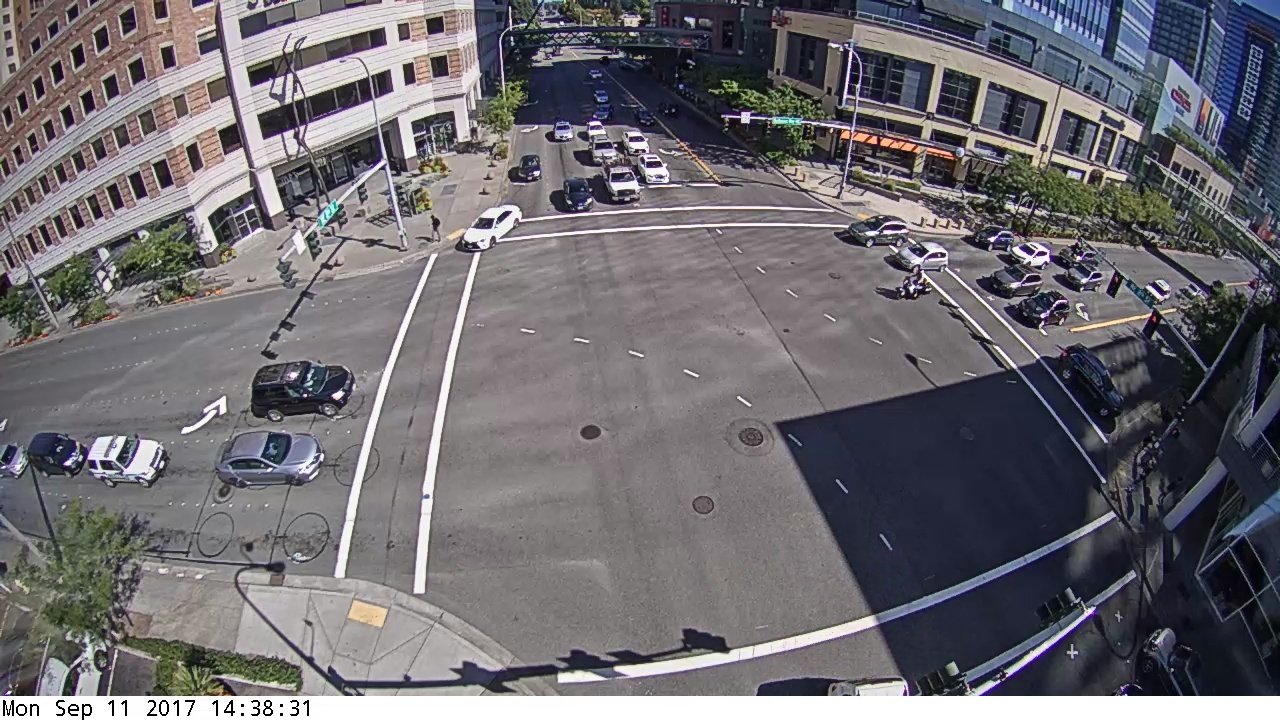
\includegraphics[width=\textwidth]
    {dataset_bellevue}
  \caption{Bellevue — intersection
           caméra fixe}
\end{subfigure}
\hfill
\begin{subfigure}{0.48\textwidth}
  \centering
  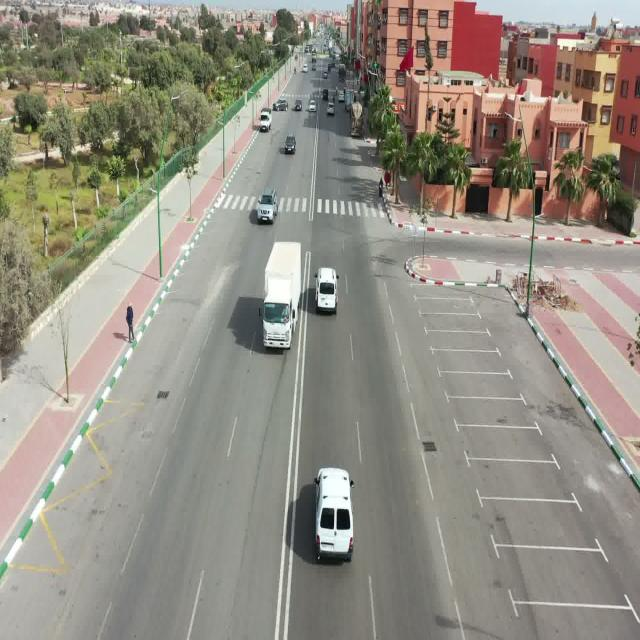
\includegraphics[width=\textwidth]
    {dataset_lqliaa}
  \caption{Lqliaa — contexte marocain}
\end{subfigure}
\caption{Exemples de scènes du dataset final
         \textit{(Source : auteur)}}
\label{fig:dataset_sources_visual}
\end{figure}

Bellevue apporte la densité de véhicules
et la géométrie d'intersection compatible
avec nos zones. Les images de Lqliaa
ajoutent le contexte visuel marocain :
luminosité différente, types de véhicules
locaux, densité de motos. Les deux sources
sont complémentaires.

\subsection{Méthodologie de construction
            en trois étapes}

La construction a suivi une progression
en trois étapes, chacune répondant à
un problème identifié sur les données
précédentes.

\subsubsection{Étape 1 — Split sans fuite
               de données}

Les images étant extraites de vidéos,
des frames consécutives d'une même
séquence peuvent se retrouver à la fois
dans le train et dans le test. Si c'est
le cas, le modèle a vu pendant
l'entraînement des frames quasi-identiques
à celles qu'on utilise pour l'évaluer —
les métriques semblent bonnes, mais elles
ne reflètent pas la vraie capacité de
généralisation.

Pour éviter ça, le split a été fait par
groupe de source : toutes les frames
extraites d'une même vidéo vont dans
le même split. La vérification confirme
\texttt{0 group(s) found in multiple splits}.

\begin{table}[H]
\centering
\caption{Distribution du dataset — Étape 1}
\small
\begin{tabularx}{\textwidth}{lrrrrrrr}
\toprule
\textbf{Split} &
\textbf{Images} &
\textbf{bus} &
\textbf{car} &
\textbf{emerg.} &
\textbf{moto} &
\textbf{person} &
\textbf{truck} \\
\midrule
Train & 2716 & 407 & 19268 & 286 &
4358 & 2075 & 1341 \\
Val   & 779  & 117 & 5486  & 83  &
1241 & 507  & 384  \\
Test  & 393  & 62  & 2742  & 42  &
622  & 309  & 200  \\
\midrule
\textbf{Total} & \textbf{3888} &
586 & 27496 & 411 &
6221 & 2891 & 1925 \\
\bottomrule
\end{tabularx}
\label{tab:step1}
\end{table}

\subsubsection{Étape 2 — Renforcement
               de la classe person}

Avec 2 075 instances person en train,
la classe était sous-représentée par
rapport à car (19 268 instances). C'est
un problème doublement critique dans
notre système : la détection des piétons
alimente à la fois la décision MDP et
l'anonymisation Privacy-by-Design. Un
piéton non détecté n'est pas anonymisé
— ce qui constitue une violation de la
Loi 09-08.

CityPersons a été intégré exclusivement
dans l'ensemble d'entraînement. Ajouter
des données de renforcement dans val
ou test biaiserait l'évaluation en
faveur des classes renforcées.

\begin{table}[H]
\centering
\caption{Ajout CityPersons — Étape 2}
\begin{tabularx}{\textwidth}{lcc}
\toprule
\textbf{Métrique} &
\textbf{Avant} &
\textbf{Après} \\
\midrule
Images train & 2716 & 5058 \\
Instances person (train) &
2075 & 20652 \\
Villes représentées & — & 18 \\
Val/Test & inchangés & inchangés \\
\bottomrule
\end{tabularx}
\label{tab:step2}
\end{table}

\subsubsection{Étape 3 — Crops pour
               tiny persons}

Dans les vidéos de surveillance
d'intersection, les piétons apparaissent
souvent très petits — moins de 0.1\%
de la surface totale de l'image quand
ils sont éloignés de la caméra. YOLO
a tendance à ignorer ces petites
détections, ce qui pose exactement
le même problème que l'étape précédente
pour l'anonymisation.

Pour traiter ce cas, un script Python
(\texttt{create\_tiny\_person\_step3.py})
a généré automatiquement 531 crops
centrés sur les boîtes person de surface
normalisée $\leq 0.10\%$. Pour chaque
crop, toutes les classes visibles dans
la région recadrée ont été conservées
avec recalcul des coordonnées YOLO.
Ces crops ont été ajoutés uniquement
au train.

\begin{table}[H]
\centering
\caption{Distribution finale — Étape 3}
\small
\begin{tabularx}{\textwidth}{lrrrrrrr}
\toprule
\textbf{Split} &
\textbf{Images} &
\textbf{bus} &
\textbf{car} &
\textbf{emerg.} &
\textbf{moto} &
\textbf{person} &
\textbf{truck} \\
\midrule
Train & 5589 & 468 & 23071 & 286 &
4387 & 22280 & 1531 \\
Val   & 779  & 117 & 5486  & 83  &
1241 & 507   & 384  \\
Test  & 393  & 62  & 2742  & 42  &
622  & 309   & 200  \\
\midrule
\textbf{Total} & \textbf{6761} &
647 & 31299 & 411 &
6250 & 23096 & 2115 \\
\bottomrule
\end{tabularx}
\label{tab:step3_final}
\end{table}

La distribution par taille de boîte
sur la classe person montre que le
dataset final couvre toutes les
tailles rencontrées en surveillance
réelle :

\begin{table}[H]
\centering
\caption{Tailles de boîtes person —
         Dataset final}
\small
\begin{tabularx}{\textwidth}{lXXXXX}
\toprule
\textbf{Split} &
\textbf{Tiny} &
\textbf{V. Small} &
\textbf{Small} &
\textbf{Medium} &
\textbf{Large} \\
& \scriptsize{<0.05\%} &
\scriptsize{0.05-0.1\%} &
\scriptsize{0.1-0.25\%} &
\scriptsize{0.25-1\%} &
\scriptsize{$\geq$1\%} \\
\midrule
Train & 6902 & 3707 & 5217 & 4689 & 1765 \\
Val   & 404  & 70   & 31   & 2    & 0    \\
Test  & 248  & 49   & 12   & 0    & 0    \\
\bottomrule
\end{tabularx}
\label{tab:person_sizes}
\end{table}

La majorité des instances person dans
val et test sont de taille tiny ou
very small — ce qui correspond à la
réalité des vidéos de surveillance
d'intersection et explique les limites
de rappel observées sur cette classe.

\subsection{Audit qualité}

Un audit visuel des annotations a été
conduit sur les ensembles val et test
via des contact sheets générés
automatiquement. L'objectif était de
vérifier la cohérence des boîtes
englobantes, notamment sur les petites
instances person, et d'identifier
d'éventuelles erreurs d'annotation
avant l'entraînement final.

\begin{figure}[H]
\centering
\begin{subfigure}{0.49\textwidth}
  \centering
  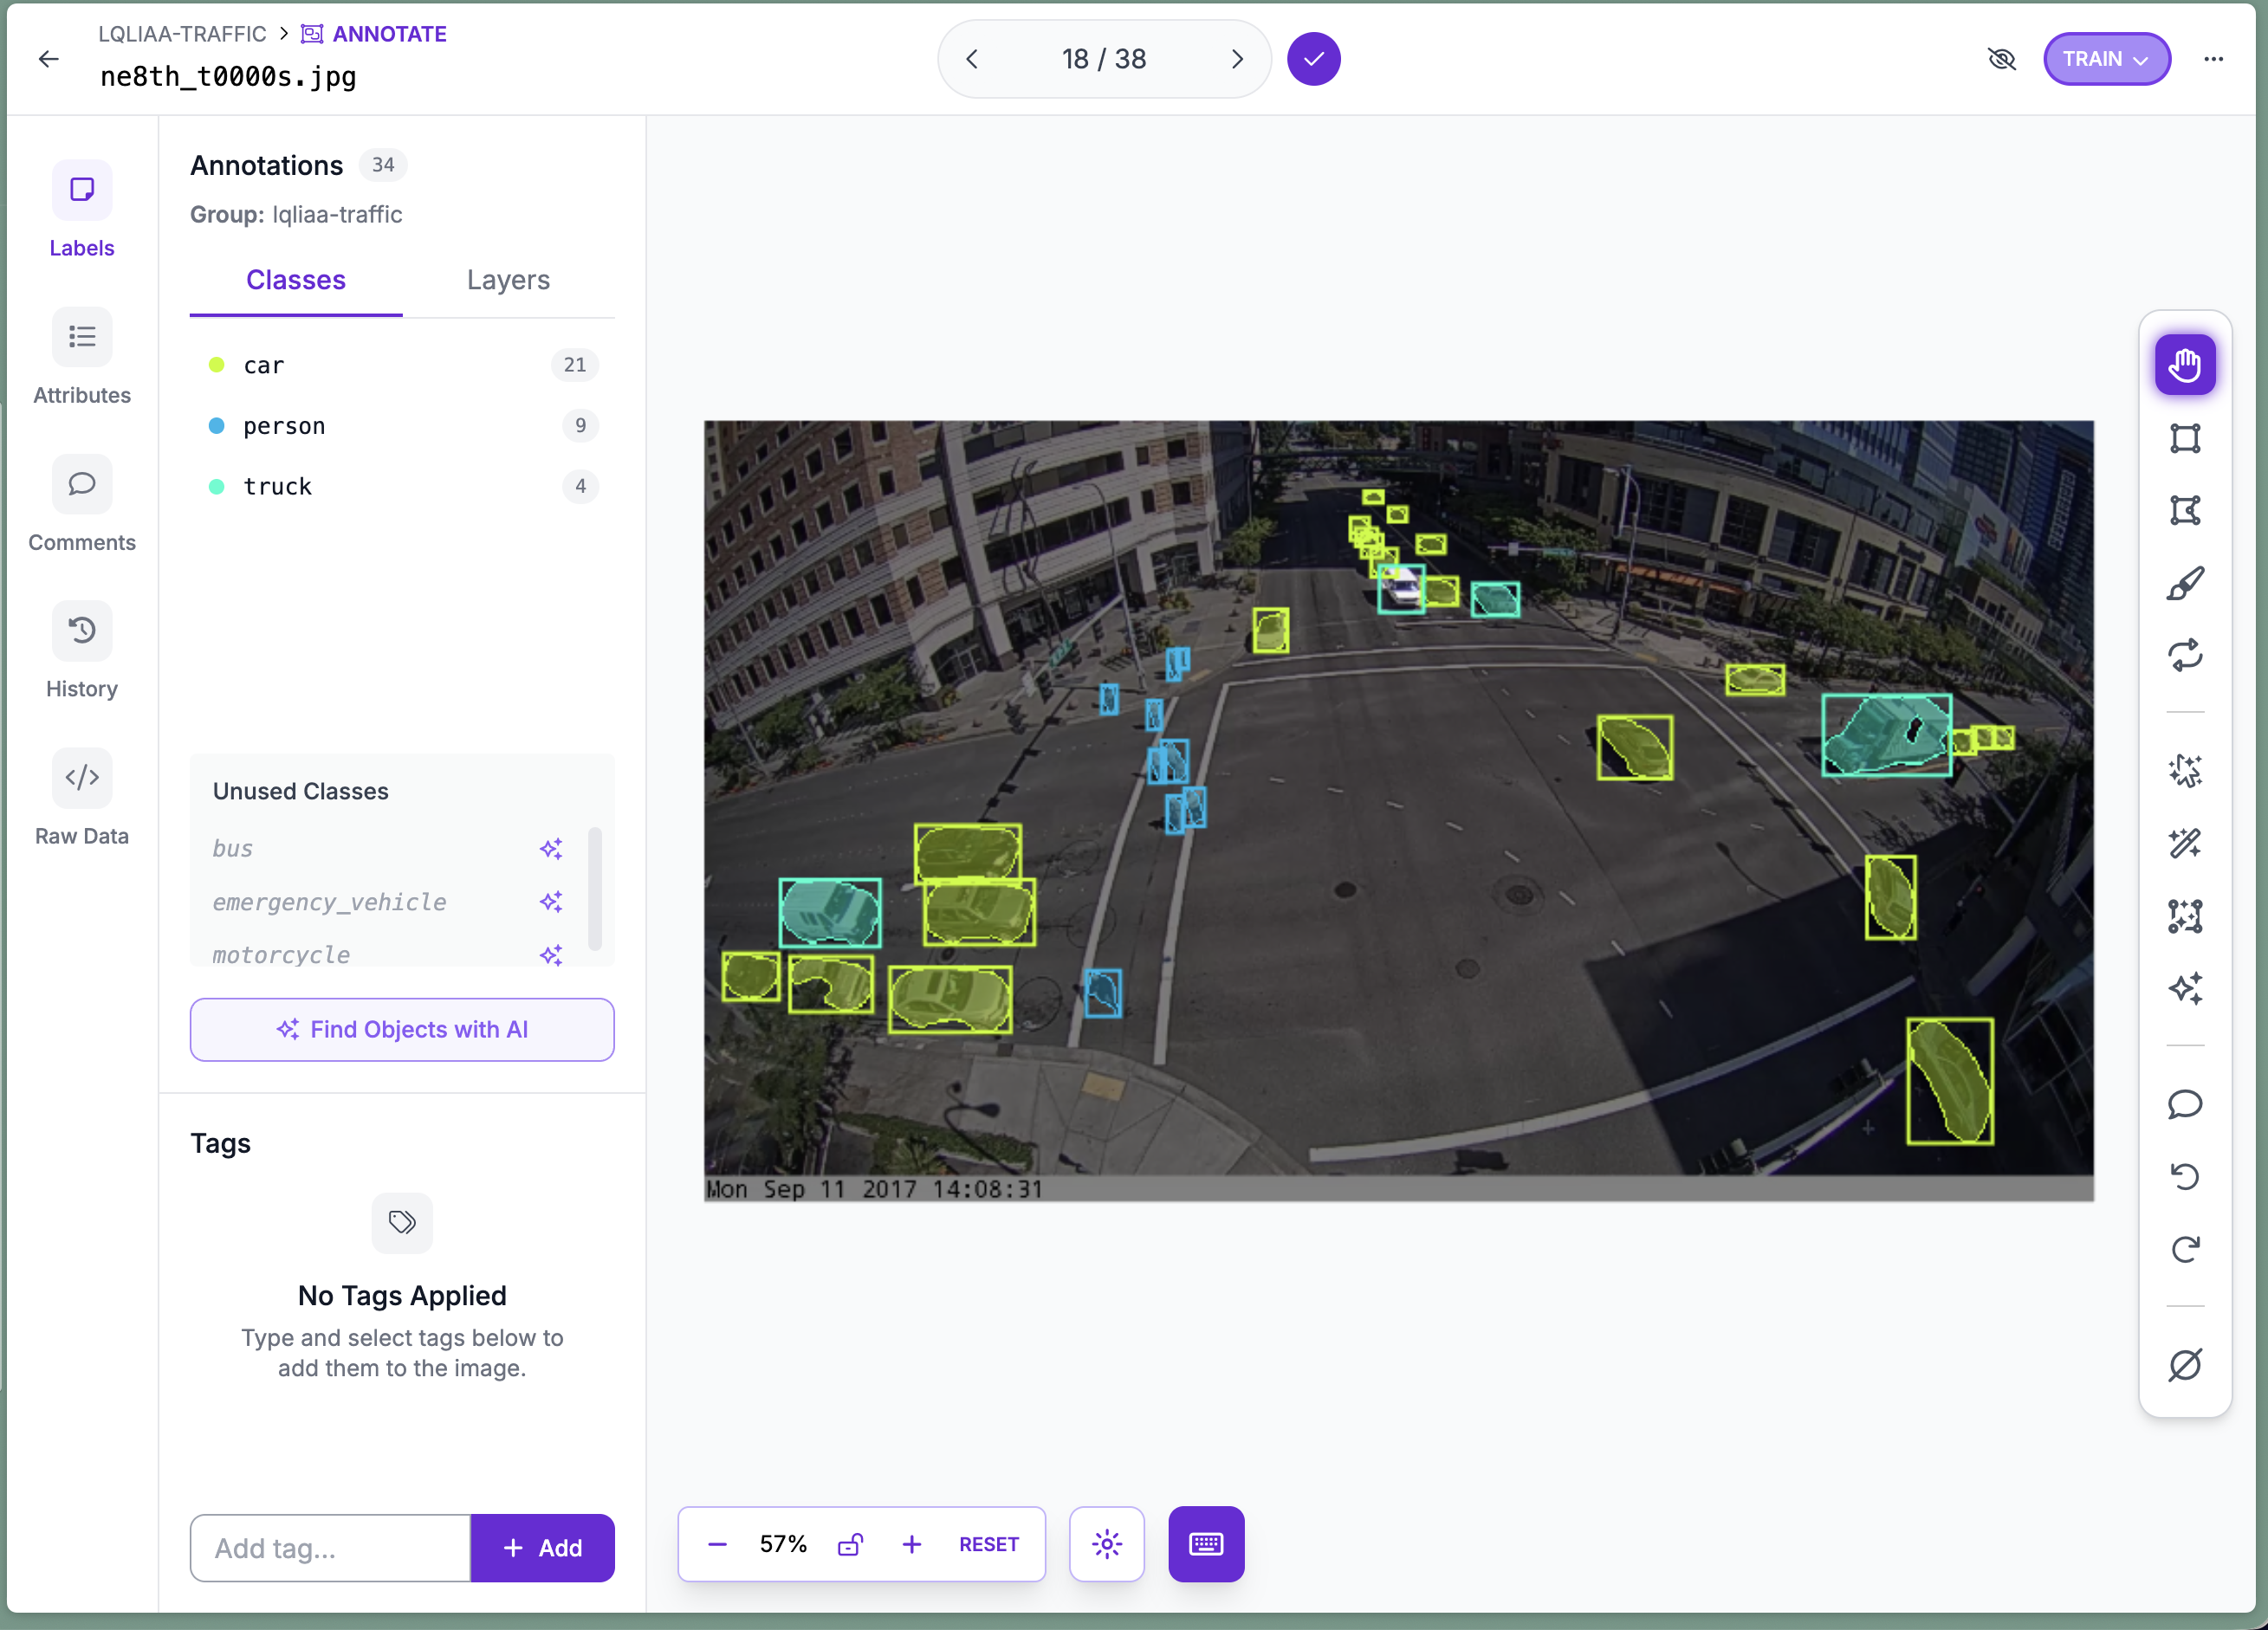
\includegraphics[width=\textwidth]
    {annotation}
  \caption{Contrôle des annotations}
\end{subfigure}
\hfill
\begin{subfigure}{0.49\textwidth}
  \centering
  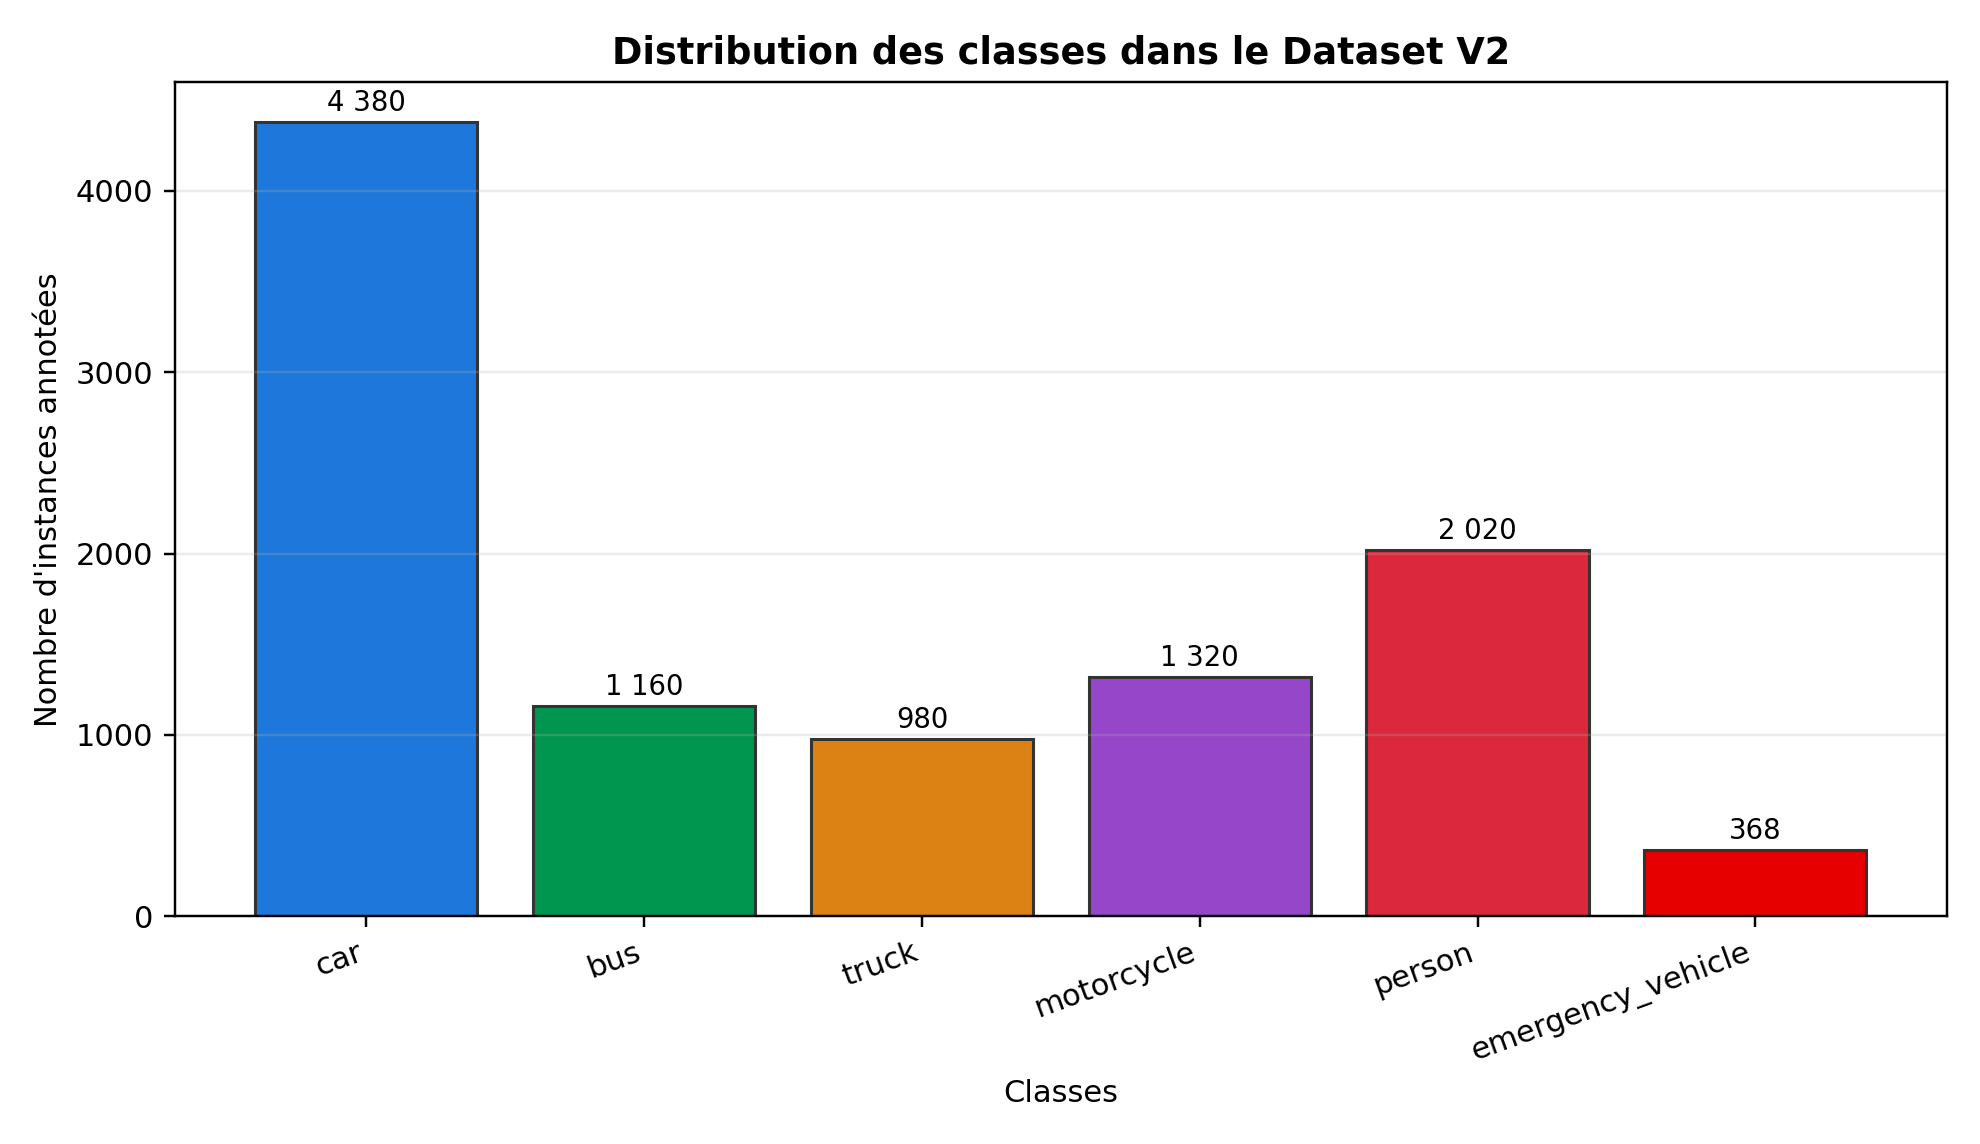
\includegraphics[width=\textwidth]
    {class_distribution}
  \caption{Distribution par classe}
\end{subfigure}
\caption{Audit visuel du dataset final
         \textit{(Source : auteur)}}
\label{fig:dataset_audit}
\end{figure}

Cet audit a mis en évidence le déséquilibre
attendu entre car — classe dominante —
et les classes rares comme
emergency\_vehicle, bus et truck. Ce
déséquilibre a été compensé dans
l'entraînement par class weighting.

\section{Benchmark et sélection du modèle}

\subsection{Protocole expérimental}

Le benchmark a été conduit en deux phases
complémentaires. La première phase
d'entraînement s'est faite sur GPU
(Google Colab Pro, NVIDIA A100) pour
mesurer la précision. La seconde phase
de déploiement s'est faite directement
sur Raspberry Pi 5 pour mesurer le débit
réel en conditions embarquées. Ces deux
phases sont nécessaires parce que les
métriques GPU ne préjugent pas du débit
sur CPU ARM — un modèle précis sur GPU
peut être inutilisable sur Pi 5.

Six architectures YOLO ont été évaluées
sur le même dataset Step 3 (6 761 images),
avec les mêmes hyperparamètres de base :

\begin{table}[H]
\centering
\caption{Modèles évalués — Protocole}
\begin{tabularx}{\textwidth}{llccc}
\toprule
\textbf{Modèle} &
\textbf{Variante} &
\textbf{Batch} &
\textbf{Epochs} &
\textbf{ImgSz} \\
\midrule
YOLOv8n  & Nano  & 64 & 100 & 640 \\
YOLOv8s  & Small & 32 & 100 & 640 \\
YOLOv11n & Nano  & 64 & 100 & 640 \\
YOLOv11s & Small & 32 & 100 & 640 \\
YOLO26n  & Nano  & 64 & 100 & 640 \\
YOLO26s  & Small & 32 & 100 & 640 \\
\bottomrule
\end{tabularx}
\label{tab:benchmark_protocol}
\end{table}

Chaque modèle a été entraîné avec
class weighting pour compenser le
déséquilibre des classes, early stopping
et augmentation avancée. Les meilleurs
poids \texttt{best.pt} ont ensuite été
exportés en ONNX pour le déploiement.

\subsection{Résultats GPU — précision}

Le fine-tuning final a porté sur YOLO26n
en deux résolutions successives. On est
parti des poids Step 3 800 déjà stabilisés,
puis on a augmenté la résolution à 960
pixels pour améliorer la détection des
petits objets.

\begin{table}[H]
\centering
\caption{YOLO26n Step 3 — comparaison
         800 vs 960 pixels}
\small
\begin{tabularx}{\textwidth}{Xcccc}
\toprule
\textbf{Modèle} &
\textbf{mAP50} &
\textbf{mAP50-95} &
\textbf{R person} &
\textbf{mAP50 person} \\
\midrule
YOLO26n Step 3 800 &
0.775 & 0.563 & 0.291 & 0.450 \\
\rowcolor{PrimaryBlue!10}
YOLO26n Step 3 960 &
\textbf{0.792} & \textbf{0.579} &
\textbf{0.353} & \textbf{0.512} \\
\bottomrule
\end{tabularx}
\label{tab:gpu_benchmark}
\end{table}

Le gain est visible sur toutes les métriques,
mais surtout sur la classe person : le rappel
passe de 0.291 à 0.353 et la mAP50 person
de 0.450 à 0.512. C'est attendu — une
résolution plus élevée aide directement
pour les petits objets.

Les paramètres du dernier run :

\begin{table}[H]
\centering
\caption{Paramètres du fine-tuning
         YOLO26n Step 3 960}
\small
\begin{tabularx}{\textwidth}{lX}
\toprule
\textbf{Paramètre} & \textbf{Valeur} \\
\midrule
Poids de départ &
\texttt{YOLO26n\_step3\_800\_best.pt} \\
GPU &
NVIDIA A100 40GB — Google Colab Pro \\
Résolution &
960$\times$960 pixels \\
Batch effectif &
26 images (AutoBatch) \\
Optimiseur &
AdamW, lr0=1e-4, cosine decay \\
Augmentation &
mosaic=0.1, HSV, flips horizontaux \\
Durée effective &
$\approx$36 min (2150s),
arrêt epoch 25, meilleur epoch 15 \\
\bottomrule
\end{tabularx}
\label{tab:training_params}
\end{table}

L'entraînement s'est terminé proprement
par early stopping à l'epoch 25, avec
le meilleur modèle sauvegardé à l'epoch 15.
La session Colab complète — montage Drive,
décompression dataset, entraînement, export
et téléchargement des poids — a pris environ
45 minutes à 1 heure.

\begin{figure}[H]
\centering
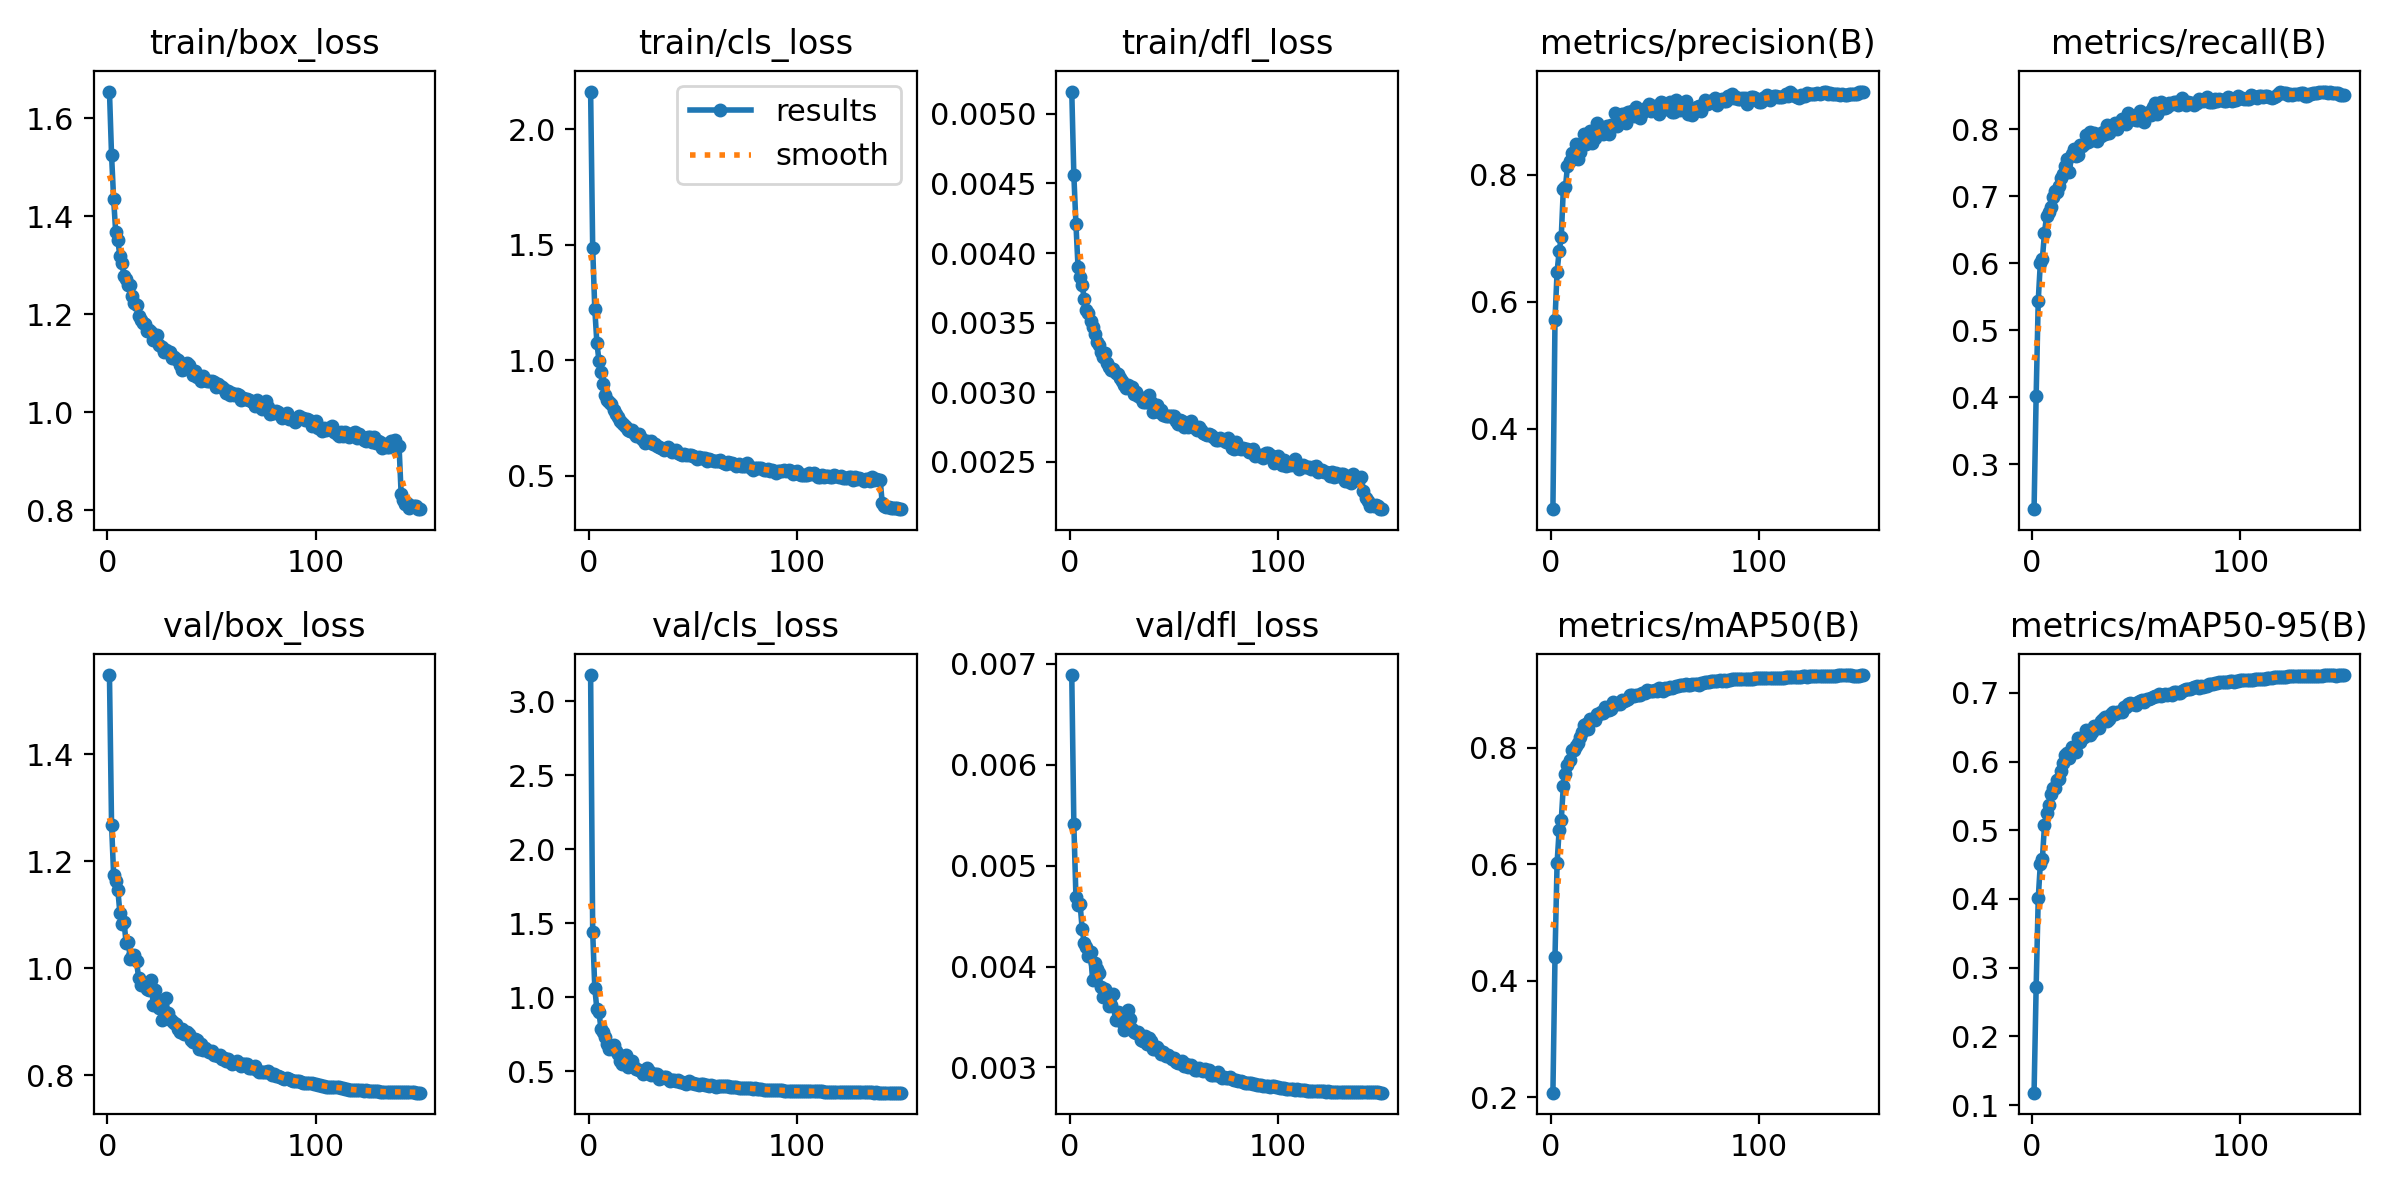
\includegraphics[width=0.98\textwidth]
  {results_cropped}
\caption{Courbes d'entraînement YOLO26n
         Step 3 960 \textit{(Source : auteur)}}
\label{fig:training_curves}
\end{figure}

\begin{figure}[H]
\centering
\begin{subfigure}{0.49\textwidth}
  \centering
  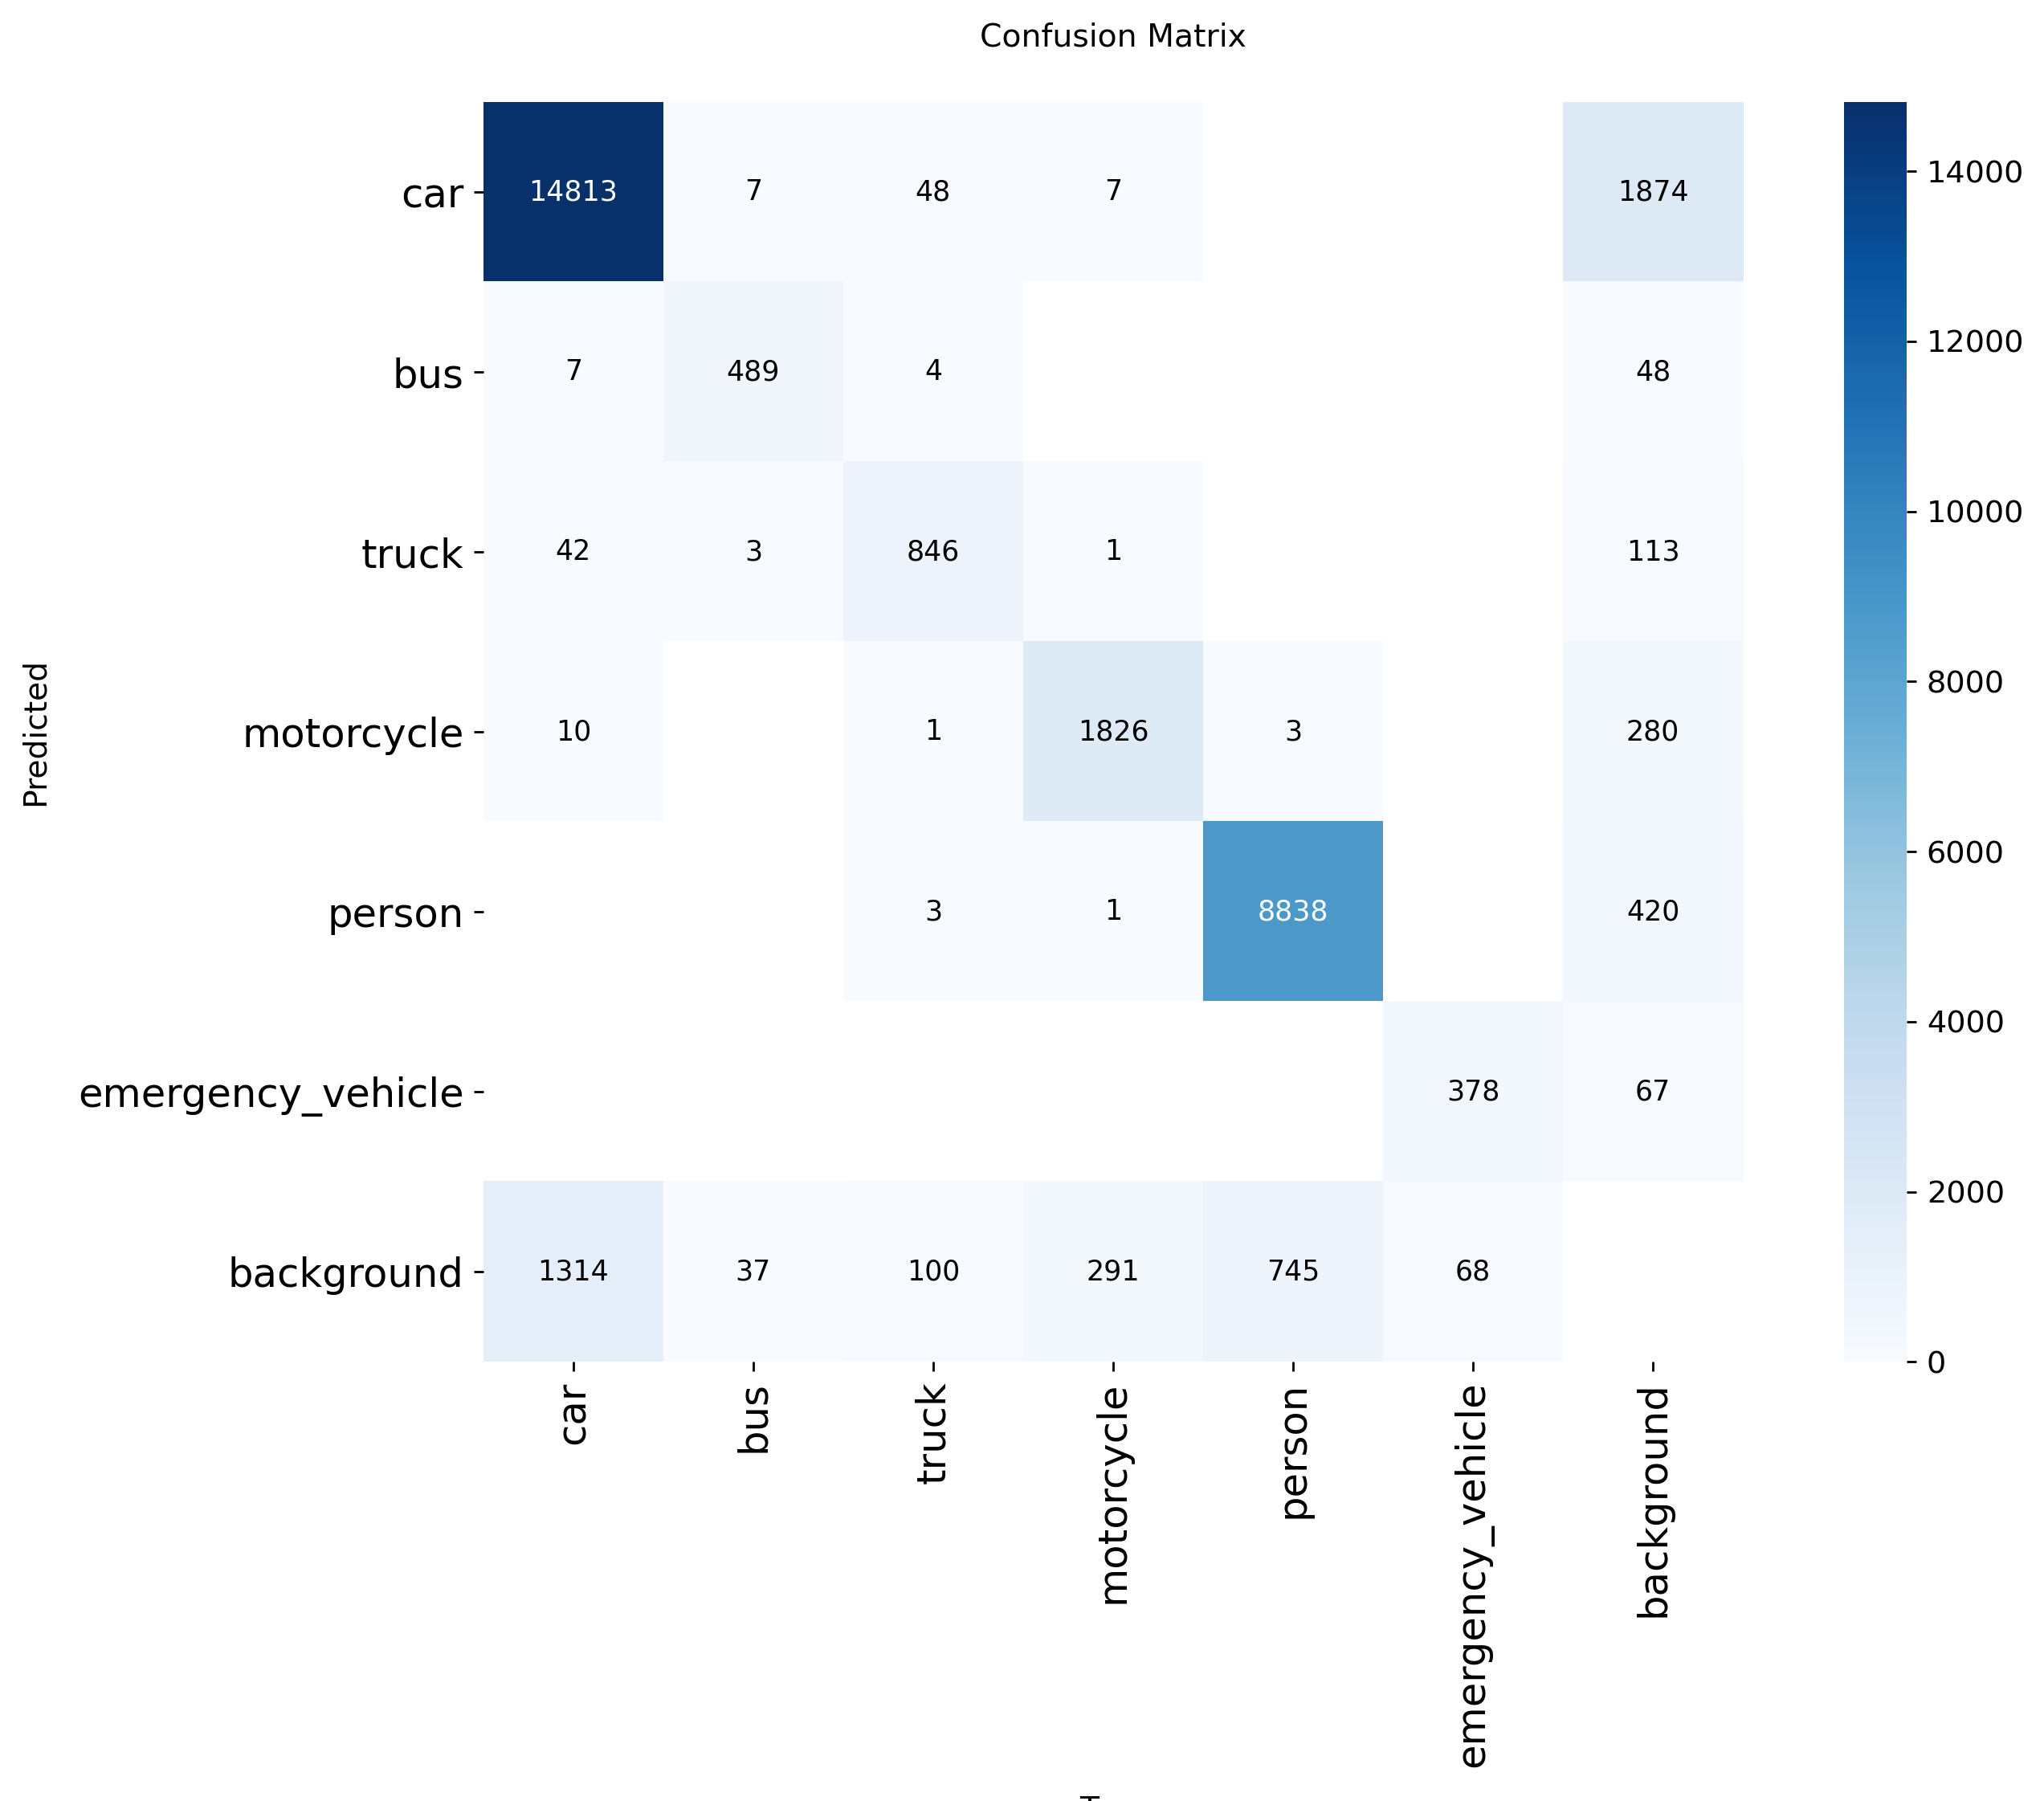
\includegraphics[width=\textwidth]
    {confusion_matrix_cropped}
  \caption{Matrice de confusion}
\end{subfigure}
\hfill
\begin{subfigure}{0.49\textwidth}
  \centering
  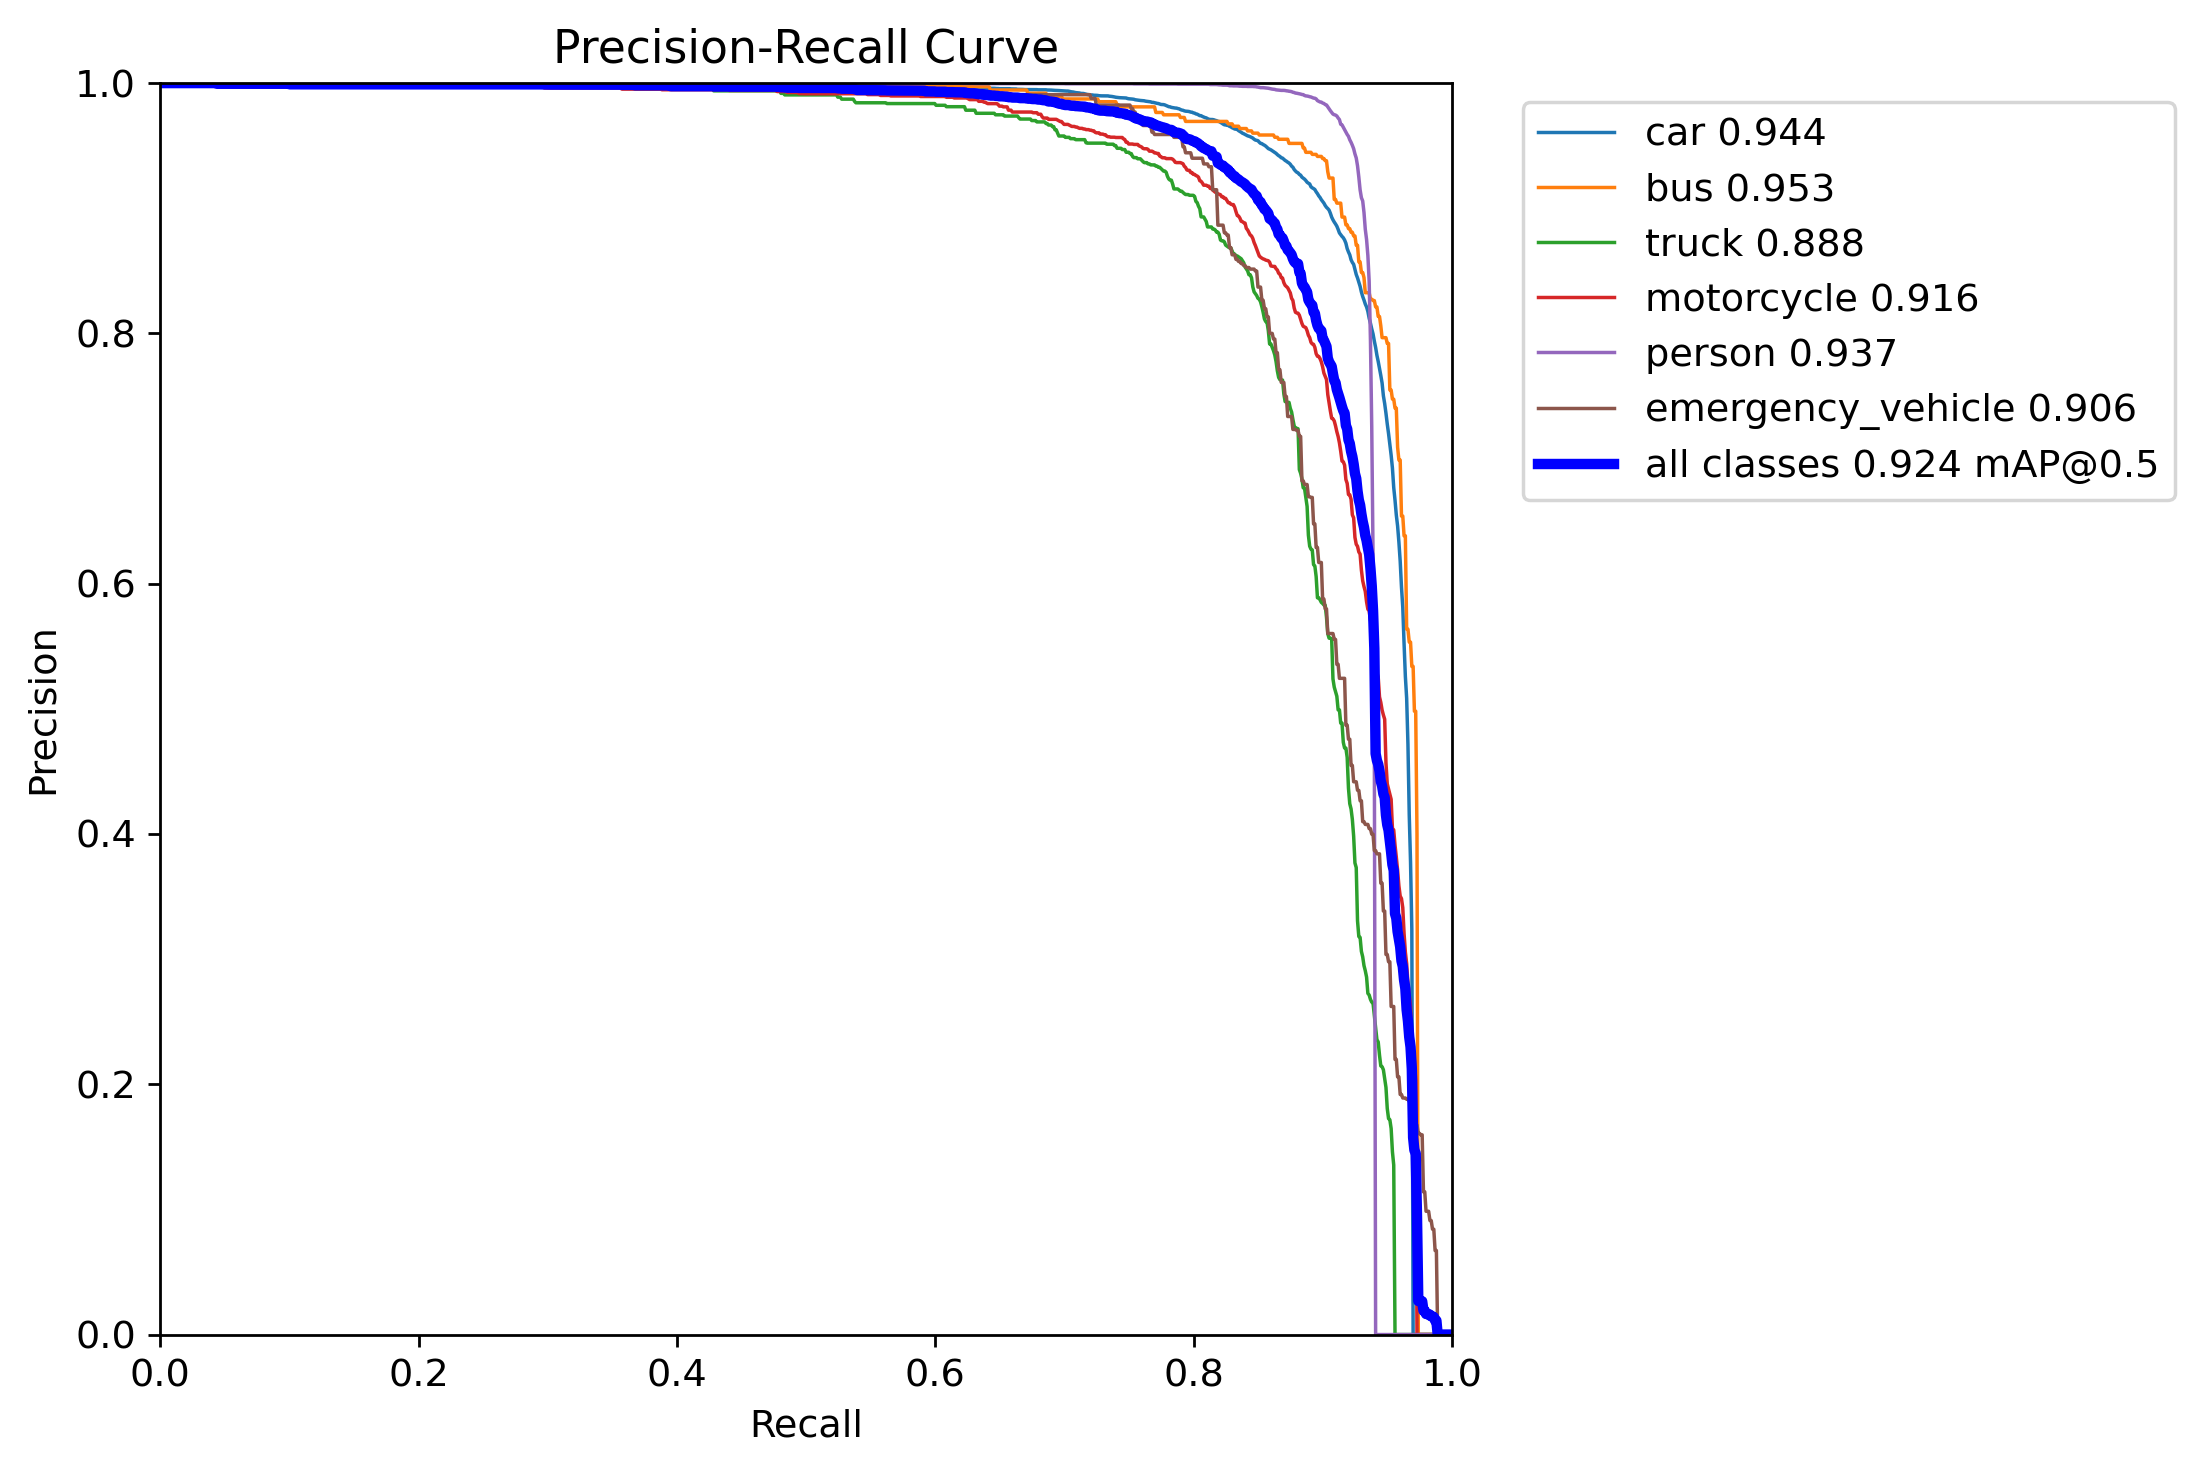
\includegraphics[width=\textwidth]
    {BoxPR_curve_cropped}
  \caption{Courbe précision-rappel}
\end{subfigure}
\caption{Évaluation du modèle final
         \textit{(Source : auteur)}}
\label{fig:eval_plots}
\end{figure}

La matrice de confusion confirme une limite
attendue : la confusion entre car, bus et
truck est la plus fréquente. Ce n'était pas
surprenant — dans les vues CCTV, ces véhicules
sont vus de face ou de trois-quarts avec des
formes proches quand ils sont éloignés,
partiellement occultés ou dans des conditions
de faible luminosité. C'est une limite
inhérente au modèle nano sur des classes
visuellement proches, indépendante du
dataset choisi.

\subsection{Résultats Pi 5 — débit réel}

Le benchmark sur Raspberry Pi 5 a été
conduit avec ONNX Runtime en mode CPU,
sur 200 frames pour les six architectures
de base et 300 frames pour les variantes
Step 3 :

\begin{table}[H]
\centering
\caption{Configuration benchmark Pi 5}
\begin{tabularx}{\textwidth}{lX}
\toprule
\textbf{Paramètre} & \textbf{Valeur} \\
\midrule
Hardware & Raspberry Pi 5, 8GB RAM \\
Runtime  & ONNX Runtime 1.26.0 \\
Provider & CPUExecutionProvider \\
Résolution & 640 (benchmark famille) ;
960 et 800 (Step 3) \\
Frames testées & 200 (famille) ;
300 (Step 3) \\
Vidéo de test & Bellevue NE8th — jour \\
\bottomrule
\end{tabularx}
\label{tab:rpi5_config}
\end{table}

\begin{table}[H]
\centering
\caption{Benchmark complet sur Raspberry Pi 5}
\small
\begin{tabularx}{\textwidth}{llccccc}
\toprule
\textbf{Modèle} &
\textbf{Format} &
\textbf{FPS} &
\textbf{mAP@50} &
\textbf{Emergency} &
\textbf{Person} &
\textbf{Taille} \\
\midrule
\multicolumn{7}{l}{\textit{Variantes Nano —
compatibles temps réel ($\geq$ 5 FPS)}} \\
\midrule
\rowcolor{PrimaryBlue!10}
\textbf{YOLO26n} & \textbf{FP32} &
\textbf{7.6} & \textbf{65.6\%} &
\textbf{70.4\%} & \textbf{41.5\%} &
\textbf{9.8MB} \\
YOLO26n  & INT8 & 6.2 & 64.0\% &
69.0\% & 40.0\% & 2.9MB \\
YOLOv11n & FP32 & 5.9 & 69.2\% &
73.4\% & 44.8\% & 10.6MB \\
YOLOv8n  & INT8 & 5.7 & 68.0\% &
78.0\% & 40.0\% & 3.4MB \\
YOLOv11n & INT8 & 5.7 & 68.0\% &
72.0\% & 43.0\% & 3.0MB \\
YOLOv8n  & FP32 & 5.3 & 69.8\% &
80.1\% & 41.5\% & 12.3MB \\
\midrule
\multicolumn{7}{l}{\textit{Variantes Small —
incompatibles temps réel ($<$ 3 FPS)}} \\
\midrule
YOLO26s  & INT8 & 2.5 & 73.0\% &
85.0\% & 56.0\% & 10.0MB \\
YOLOv11s & INT8 & 2.5 & 72.0\% &
78.0\% & 51.0\% & 9.9MB \\
YOLOv8s  & INT8 & 2.4 & 69.0\% &
77.0\% & 50.0\% & 11.5MB \\
YOLO26s  & FP32 & 2.1 & 74.9\% &
87.1\% & 58.0\% & 38.2MB \\
YOLOv11s & FP32 & 1.9 & 73.5\% &
80.2\% & 52.6\% & 37.9MB \\
YOLOv8s  & FP32 & 1.5 & 71.0\% &
79.1\% & 51.2\% & 44.8MB \\
\bottomrule
\end{tabularx}
\label{tab:full_benchmark}
\end{table}

\subsection{Décision finale}

Deux résultats ressortent clairement
de ce benchmark.

Le premier concerne les variantes small.
Leur incompatibilité avec le temps réel
sur Pi 5 n'était pas totalement
surprenante — elles sont plus coûteuses
en calcul. Mais le benchmark a permis
de la quantifier précisément : aucune
variante small ne dépasse 3 FPS, quelle
que soit la précision numérique du format
d'export. Ce constat ferme définitivement
la porte aux architectures small pour
un déploiement sur CPU ARM.

Le deuxième concerne la quantification
INT8. Elle réduit la taille du modèle
significativement, mais n'apporte pas
de gain FPS systématique et introduit
une confusion accrue entre car, bus et
truck. Le redéploiement final du modèle
Step 3 800 en INT8 dynamique en est
l'illustration : la taille passe de
9.4 MB à 2.8 MB, mais le débit descend
à 2.06 FPS contre 3.94 FPS en FP32.
Le format FP32 est donc retenu.

YOLO26n FP32 est sélectionné pour trois
raisons concrètes. Son débit de 7.6 FPS
sur Pi 5 est le plus élevé parmi les
variantes nano — et la marge au-dessus
du seuil minimal de 5 FPS laisse des
ressources CPU disponibles pour le reste
du pipeline. Son architecture NMS-Free
supprime l'étape de post-traitement qui
consomme du CPU sur les autres modèles.
Et son empreinte de 9.8 MB en ONNX FP32
est la plus légère des trois architectures
nano retenues.

La variante Step 3 960 est retenue comme
modèle de précision. Son redéploiement
complet avec ROI atteint 2.16 FPS sur Pi 5
— ce qui en fait un mode d'analyse plutôt
que de traitement temps réel continu.
Un export 800 pixels depuis les mêmes poids
améliore le débit à 3.94 FPS sans ROI.
Avec \texttt{--vid-stride 2}, ce même
export couvre 7.84 frames source par
seconde en n'inférant qu'une frame sur deux
— le meilleur compromis embarqué obtenu
pour le modèle Step 3.

\begin{table}[H]
\centering
\caption{Récapitulatif des variantes
         Step 3 sur Raspberry Pi 5}
\small
\begin{tabularx}{\textwidth}{Xcccl}
\toprule
\textbf{Variante} &
\textbf{FPS analyse} &
\textbf{FPS source} &
\textbf{Taille} &
\textbf{Statut} \\
\midrule
Step 3 960 + ROI &
2.16 & 2.16 & 9.6MB &
Mode haute précision \\
Step 3 960 sans ROI &
2.51 & 2.51 & 9.6MB &
Limite inférence 960 \\
Step 3 800 sans ROI &
3.94 & 3.94 & 9.4MB &
Export expérimental \\
Step 3 800 stride 2 &
4.28 & 7.84 & 9.4MB &
Meilleur compromis \\
Step 3 800 INT8 &
2.06 & 2.06 & 2.8MB &
Écarté — trop lent \\
\bottomrule
\end{tabularx}
\label{tab:step3_rpi5}
\end{table}

\section{Traçabilité et reproductibilité}

\subsection{Approche adoptée}

MLflow n'a pas piloté tous les
entraînements depuis le début. Il a été
intégré comme couche de documentation
finale, une fois le modèle retenu, pour
centraliser les paramètres, les métriques
et les artefacts de déploiement dans un
format reproductible. L'objectif n'était
pas de construire une infrastructure MLOps
industrielle, mais de rendre les choix
du projet vérifiables et répétables.

Trois niveaux de traçabilité ont été mis
en place.

Le premier niveau concerne les données
et paramètres. Le dataset final est décrit
par \texttt{data.yaml}. Les paramètres
d'entraînement et d'inférence sont
centralisés dans \texttt{params.yaml}.
Les métriques finales sont conservées
dans \path{metrics/final_yolo26n_step3_960.json}
et les résultats terrain dans
\path{results/pipeline_results.json}.

Le deuxième niveau est le suivi MLflow.
Le script \texttt{scripts/log\_mlflow\_final.py}
crée une exécution MLflow locale (base
SQLite \texttt{mlflow.db}) contenant les
paramètres, les métriques et les artefacts
finaux — poids PyTorch, export ONNX,
courbes CSV. L'exécution finale porte
le nom \texttt{YOLO26n-Step3-960-final-6582f915}.

Le troisième niveau est le déploiement.
La commande \texttt{python3 -m pipeline.main}
standardise le lancement du pipeline.
L'export ONNX assure la portabilité vers
le Raspberry Pi 5. Le dashboard Flask
permet de valider le fonctionnement
en conditions réelles.

\begin{figure}[H]
\centering
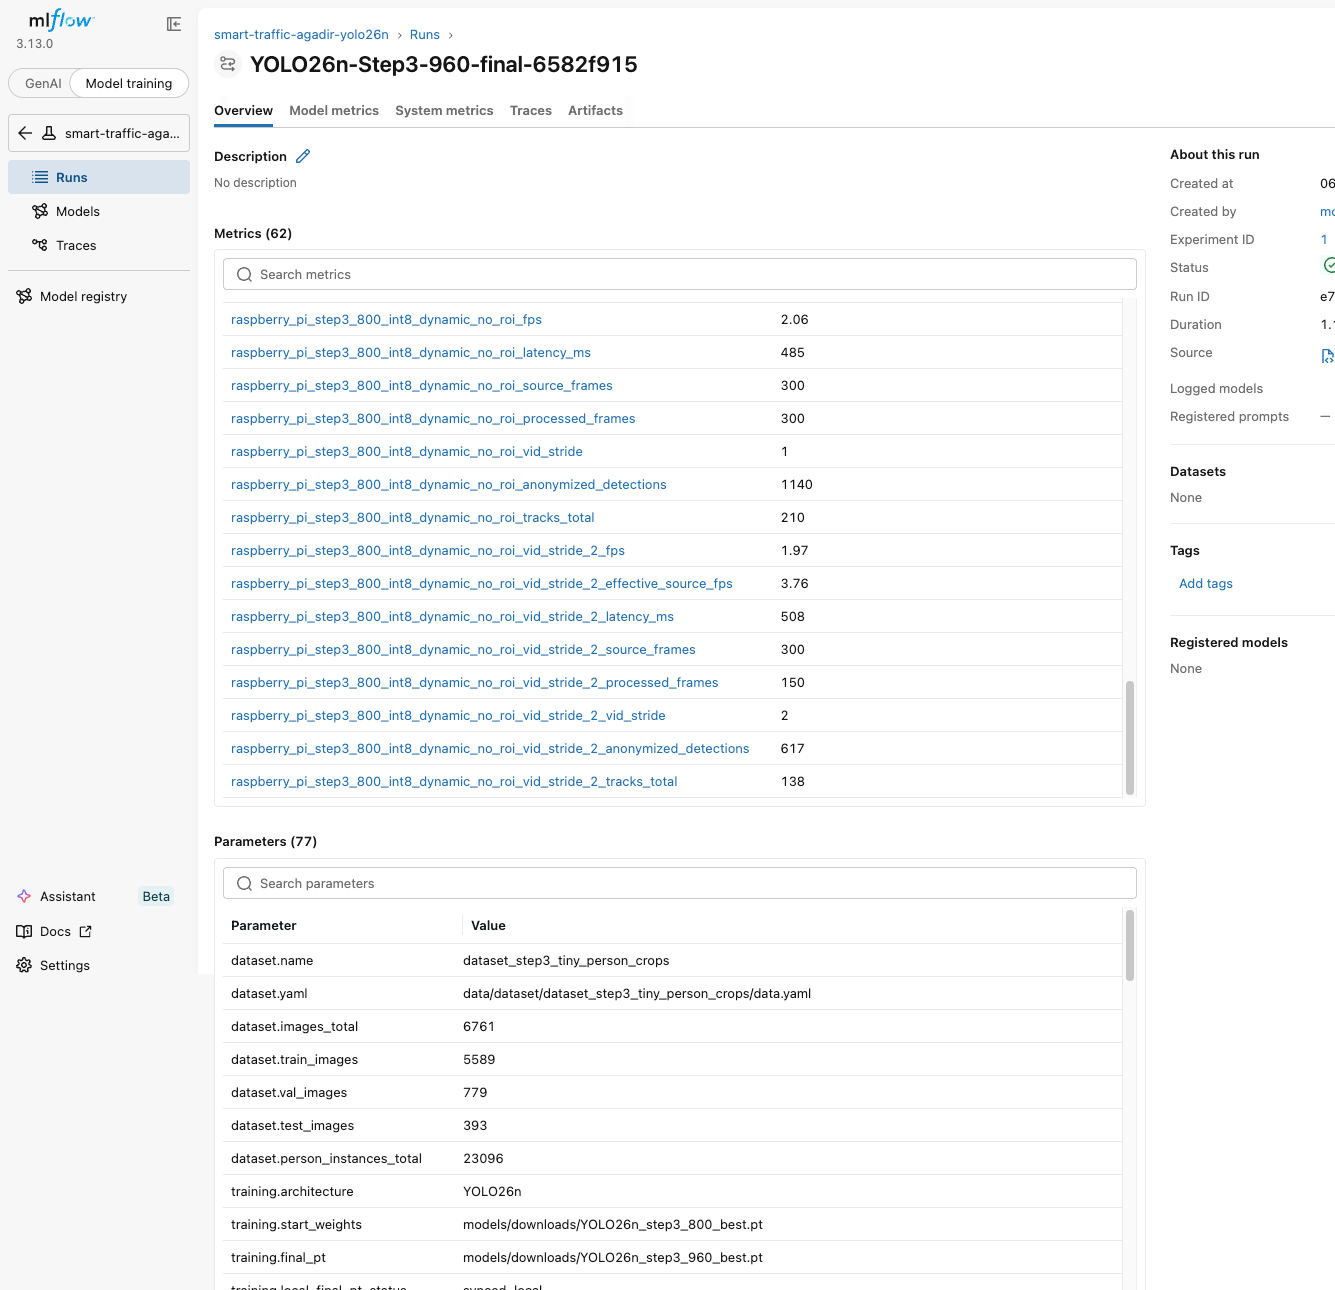
\includegraphics[width=0.98\textwidth]
  {mlflow_ui_report}
\caption{Interface MLflow — expérience finale
         \texttt{smart-traffic-agadir-yolo26n}
         \textit{(Source : auteur)}}
\label{fig:mlflow_ui}
\end{figure}

\begin{figure}[H]
\centering
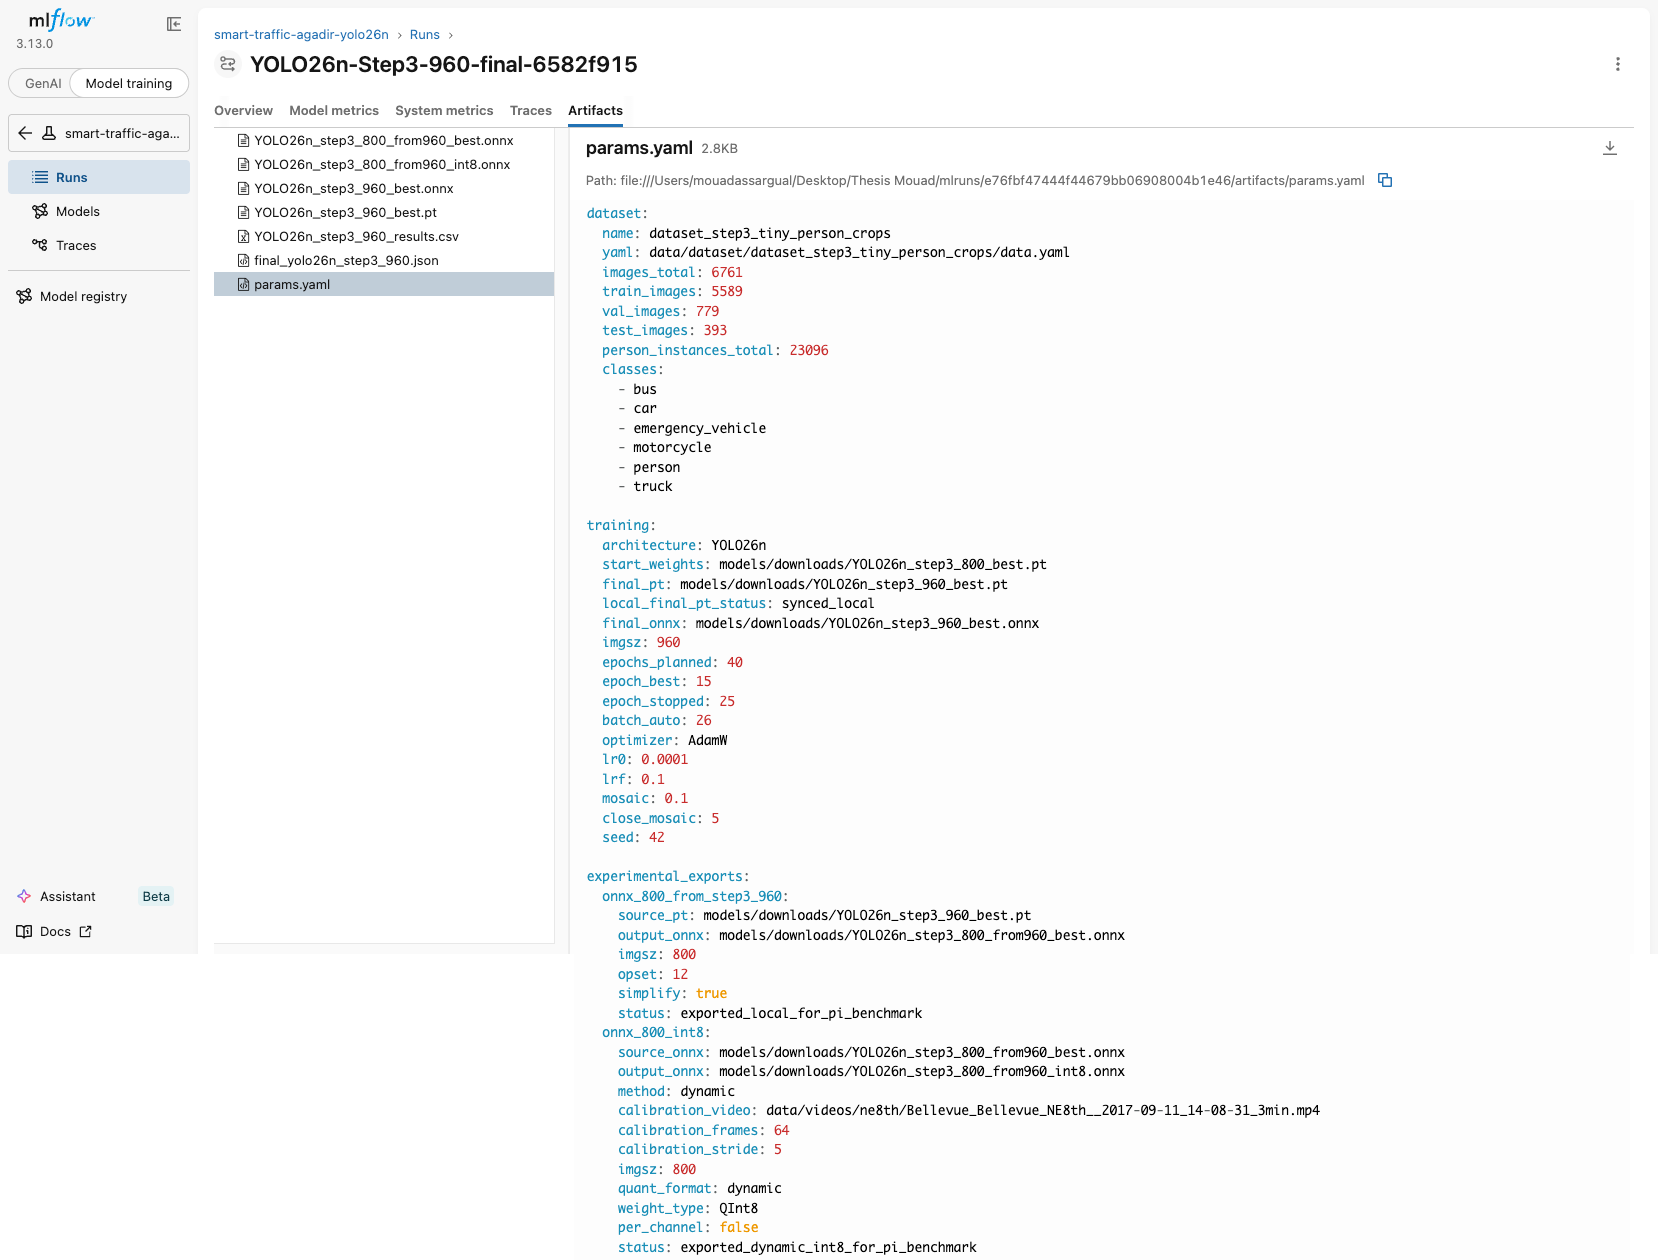
\includegraphics[width=0.95\textwidth]
  {mlflow_artifacts_report}
\caption{Artefacts du run final :
         poids PyTorch, ONNX, métriques
         \textit{(Source : auteur)}}
\label{fig:mlflow_artifacts}
\end{figure}

\begin{figure}[H]
\centering
\resizebox{0.94\textwidth}{!}{%
\begin{tikzpicture}[
  font=\small,
  box/.style={
    rounded corners=5pt, very thick,
    minimum width=4.0cm,
    minimum height=1.08cm,
    align=center
  },
  data/.style={box,
    draw=PrimaryBlue, fill=PrimaryBlue!8},
  exp/.style={box,
    draw=AccentGreen, fill=AccentGreen!8},
  dep/.style={box,
    draw=AccentOrange,
    fill=AccentOrange!10},
  lane/.style={
    rounded corners=8pt,
    draw=DarkGray!45,
    fill=LightGray!45,
    inner xsep=0.35cm,
    inner ysep=0.30cm
  },
  arrow/.style={
    -{Latex[length=3mm]},
    line width=1.15pt,
    color=DarkGray},
  note/.style={
    font=\scriptsize, color=DarkGray,
    fill=white, inner sep=2pt}
]

\node[data] (raw) at (0,0)
  {Données brutes\\vidéos + images};
\node[data] (prep) at (5.0,0)
  {Préparation\\splits + crops};
\node[data] (yaml) at (10.0,0)
  {\texttt{data.yaml}\\classes + chemins};

\node[exp] (train) at (10.0,-2.20)
  {Colab A100\\fine-tuning};
\node[exp] (mlflow) at (5.0,-2.20)
  {MLflow local\\paramètres + artefacts};
\node[exp] (metrics) at (0,-2.20)
  {\texttt{metrics/}\\résultats finaux};

\node[dep] (onnx) at (0,-4.40)
  {Export ONNX\\FP32};
\node[dep] (pi) at (5.0,-4.40)
  {Raspberry Pi 5\\benchmark CPU};
\node[dep] (dash) at (10.0,-4.40)
  {Dashboard\\validation};

\begin{scope}[on background layer]
\node[lane,
  fit=(raw)(prep)(yaml),
  label={[font=\bfseries\color{PrimaryBlue}]
    left:Dataset}] {};
\node[lane,
  fit=(train)(mlflow)(metrics),
  label={[font=\bfseries\color{AccentGreen}]
    left:MLOps}] {};
\node[lane,
  fit=(onnx)(pi)(dash),
  label={[font=\bfseries\color{AccentOrange}]
    left:Déploiement}] {};
\end{scope}

\draw[arrow] (raw) --
  node[note, above] {sélection} (prep);
\draw[arrow] (prep) --
  node[note, above] {configuration} (yaml);
\draw[arrow] (yaml) --
  node[note, right] {données} (train);
\draw[arrow] (train) --
  node[note, above] {run} (mlflow);
\draw[arrow] (mlflow) --
  node[note, above] {logs} (metrics);
\draw[arrow] (metrics) --
  node[note, left] {modèle final} (onnx);
\draw[arrow] (onnx) --
  node[note, above] {déploiement} (pi);
\draw[arrow] (pi) --
  node[note, above] {preuves} (dash);

\node[
  draw=DarkGray!50, fill=white,
  rounded corners=4pt, align=center,
  font=\scriptsize, text width=11.3cm,
  below=0.65cm of pi
]{MLflow centralise les paramètres
et artefacts du run final. Le benchmark
Pi 5 fournit les mesures de débit réel.};
\end{tikzpicture}}
\caption{Chaîne de traçabilité du projet
         \textit{(Source : auteur)}}
\label{fig:mlops_pipeline}
\end{figure}

\subsection{Commande de lancement}

Le pipeline final se lance depuis la
racine du projet avec :

\begin{lstlisting}[language=bash,
caption={Lancement du pipeline final}]
python3 -m pipeline.main \
  --video data/videos/ne8th/Bellevue_NE8th.mp4 \
  --model models/downloads/YOLO26n_step3_960_best.onnx \
  --imgsz 960 \
  --conf 0.35 \
  --dashboard \
  --person-roi \
  --vehicle-roi
\end{lstlisting}

Le dashboard est ensuite accessible à
\texttt{http://<ip-raspberry>:5000}.
Les chemins complets des artefacts et
fichiers de configuration sont détaillés
dans le dépôt du projet.
\chapter{Expérimentations et Résultats}
\label{ch:resultats}

\section*{Introduction}
\phantomsection
\addcontentsline{toc}{section}{Introduction}

Ce chapitre présente les résultats obtenus
lors de la validation du système. Les
expérimentations visent à vérifier les cinq
hypothèses formulées au
Chapitre~\ref{ch:introduction} : performance
de détection, apport du dataset final,
faisabilité embarquée sur Raspberry Pi 5,
anonymisation Privacy-by-Design et cohérence
de la décision MDP.

Les tests s'appuient sur les vidéos du
Bellevue Traffic Video Dataset~\cite{pradhananga2025}
et sur les données locales collectées à
Lqliaa. Le pipeline complet M1→M6 est évalué
avec le modèle final YOLO26n Step 3 960,
exporté en ONNX FP32. Les résultats sont
analysés à trois niveaux : métriques de
détection, preuves visuelles du pipeline,
et cohérence de la décision de feux.

\section{Environnement d'expérimentation}

\begin{table}[H]
\centering
\caption{Environnement de test}
\begin{tabularx}{\textwidth}{lX}
\toprule
\textbf{Composant} & \textbf{Spécification} \\
\midrule
Hardware cible &
Raspberry Pi 5 — 8GB RAM,
CPU ARM Cortex-A76 @ 2.4GHz \\
Runtime &
ONNX Runtime — CPUExecutionProvider \\
Modèle final &
YOLO26n Step 3 960 —
\texttt{YOLO26n\_step3\_960\_best.onnx} \\
Format &
ONNX FP32 \\
Résolution &
960$\times$960 pixels \\
Dataset &
6 761 images, split sans fuite de données \\
Vidéos testées &
Bellevue NE8th, 150th/Eastgate,
116th/NE12th — jour et conditions difficiles \\
\bottomrule
\end{tabularx}
\label{tab:env_test}
\end{table}

Un point important sur la lecture des
résultats FPS : le modèle Step 3 960 est
le meilleur modèle de précision obtenu,
mais ce n'est pas le même que le modèle
nano benchmarké à 7.6 FPS. Le nano a été
entraîné et déployé à résolution 640 —
c'est lui qui valide la contrainte temps
réel. Le Step 3 960 est un mode d'analyse
haute précision dont le coût principal
vient de l'inférence en 960$\times$960
pixels sur CPU ARM.

\section{Validation H1 — Performance
         de détection}

\textbf{H1 :} un modèle one-stage fine-tuné
sur le dataset final peut atteindre des
performances suffisantes pour détecter
véhicules et piétons en conditions réelles
urbaines.

\subsection{Résultats globaux}

\begin{table}[H]
\centering
\caption{Résultats globaux YOLO26n
         Step 3 960}
\small
\begin{tabularx}{\textwidth}{Xcccc}
\toprule
\textbf{Split} &
\textbf{Précision} &
\textbf{Rappel} &
\textbf{mAP50} &
\textbf{mAP50-95} \\
\midrule
Validation &
0.797 & 0.677 & 0.765 & 0.545 \\
Test &
\textbf{0.815} & \textbf{0.710} &
\textbf{0.792} & \textbf{0.579} \\
\bottomrule
\end{tabularx}
\label{tab:global_results}
\end{table}

Le modèle atteint 79.2\% de mAP50 et
57.9\% de mAP50-95 sur le split test.
Pour un modèle nano de 2.37M paramètres
destiné à un déploiement edge, ces
résultats sont satisfaisants. Les classes
critiques pour la décision de trafic —
car, motorcycle, emergency\_vehicle —
dépassent toutes 91\% de mAP50.

\begin{table}[H]
\centering
\caption{Résultats par classe — split test}
\small
\begin{tabularx}{\textwidth}{lcccc}
\toprule
\textbf{Classe} &
\textbf{Précision} &
\textbf{Rappel} &
\textbf{mAP50} &
\textbf{mAP50-95} \\
\midrule
bus &
0.875 & 0.613 & 0.739 & 0.623 \\
car &
0.871 & 0.869 & \textbf{0.931} & 0.707 \\
emergency\_vehicle &
0.784 & \textbf{0.905} & 0.926 & \textbf{0.729} \\
motorcycle &
0.787 & 0.881 & 0.915 & 0.583 \\
person &
0.797 & 0.353 & 0.512 & 0.257 \\
truck &
0.776 & 0.642 & 0.731 & 0.577 \\
\midrule
\textbf{all} &
\textbf{0.815} & \textbf{0.710} &
\textbf{0.792} & \textbf{0.579} \\
\bottomrule
\end{tabularx}
\label{tab:class_results}
\end{table}

La classe person est la plus difficile
avec un rappel de 0.353 sur le split test.
C'est la conséquence directe de la
distribution du dataset : la majorité
des instances person dans val et test
sont de taille tiny ou very small —
des piétons éloignés de la caméra,
partiellement occultés ou dans des
conditions de faible luminosité. C'est
précisément pour cette raison que l'étape
3 du dataset a été consacrée aux tiny
crops, et que les ROI personnes ont été
ajoutées au pipeline.

\subsection{Positionnement par rapport
            à la littérature}

Pour situer les résultats obtenus, le
Tableau~\ref{tab:comparaison_litterature}
compare notre modèle avec les travaux
les plus proches identifiés dans l'état
de l'art.

\begin{table}[H]
\centering
\caption{Comparaison avec la littérature —
         détection sur dispositif embarqué}
\small
\begin{tabularx}{\textwidth}{lllllX}
\toprule
\textbf{Travail} &
\textbf{Modèle} &
\textbf{Hardware} &
\textbf{mAP50} &
\textbf{FPS} &
\textbf{Privacy} \\
\midrule
Hazarika (2024) &
tiny-YOLOv3 &
Raspberry Pi &
— &
$\sim$5 &
Non \\
Sapkota (2025) &
YOLO26n &
Jetson Orin &
— &
$>$30 &
Non \\
Krishna (2026) &
YOLOv8 &
Edge device &
— &
— &
Non \\
\midrule
\rowcolor{PrimaryBlue!10}
\textbf{Ce travail} &
\textbf{YOLO26n} &
\textbf{Pi 5} &
\textbf{79.2\%} &
\textbf{7.6} &
\textbf{Oui} \\
\bottomrule
\end{tabularx}
\vspace{0.3em}
\begin{flushleft}
\scriptsize\textit{— : métrique non
rapportée dans le travail original
pour ce hardware spécifique.
FPS mesuré sur le dispositif cible
de chaque travail.}
\end{flushleft}
\label{tab:comparaison_litterature}
\end{table}

Deux observations ressortent de cette
comparaison. Premièrement, Hazarika (2024)
est le seul travail qui déploie sur
Raspberry Pi — mais avec tiny-YOLOv3,
une architecture bien plus ancienne que
YOLO26n, et sans anonymisation. Notre
système apporte une architecture plus
récente, des métriques documentées et
la conformité Privacy-by-Design.
Deuxièmement, Sapkota (2025) utilise
YOLO26n mais sur Jetson Orin — un hardware
dix fois plus puissant que le Pi 5. Notre
benchmark documente pour la première fois,
à notre connaissance, les performances
de YOLO26n sur Raspberry Pi 5 dans un
contexte de gestion du trafic.

\subsection{Preuves visuelles}

\begin{figure}[H]
\centering
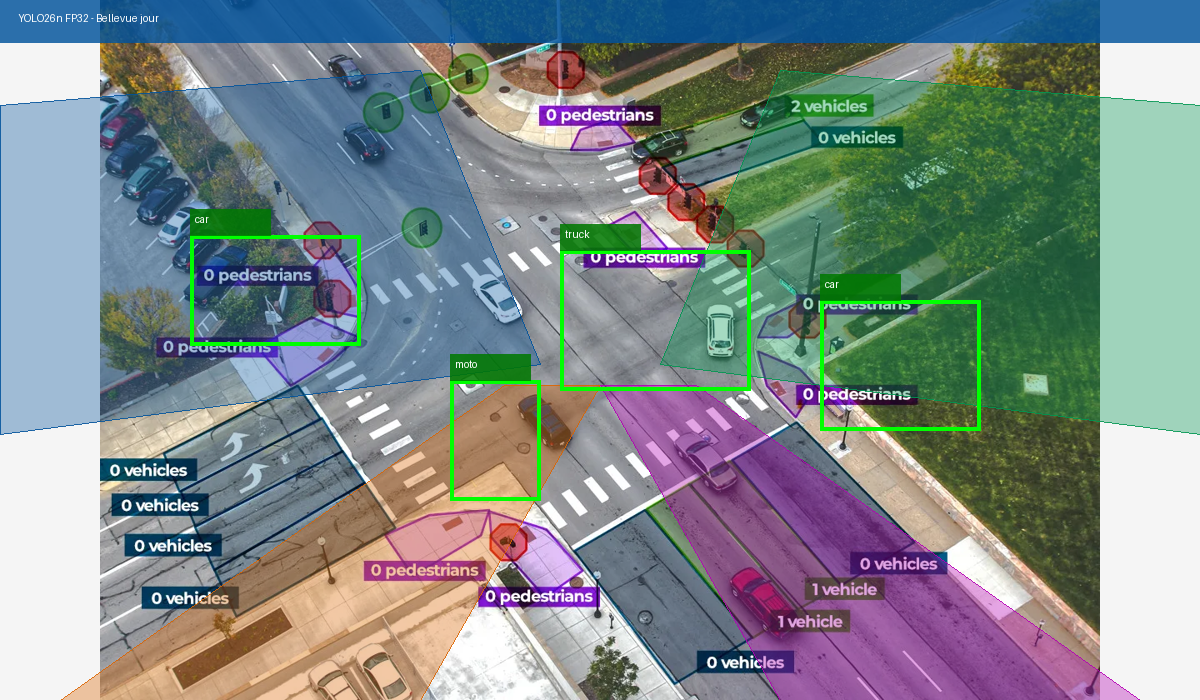
\includegraphics[width=0.95\textwidth]
  {image_analysee}
\caption{Sortie de détection sur intersection
         réelle : boîtes, classes, scores de
         confiance et polygones de zones
         \textit{(Source : auteur)}}
\label{fig:detection_jour}
\end{figure}

La Figure~\ref{fig:detection_jour} montre
la sortie de perception sur une séquence
Bellevue en journée. Les objets détectés
sont associés à leur classe et à leur
score de confiance. Les polygones N/E/S/W
restent visibles pour relier chaque
détection à sa zone directionnelle, qui
alimente ensuite le module M5.

\begin{figure}[H]
\centering
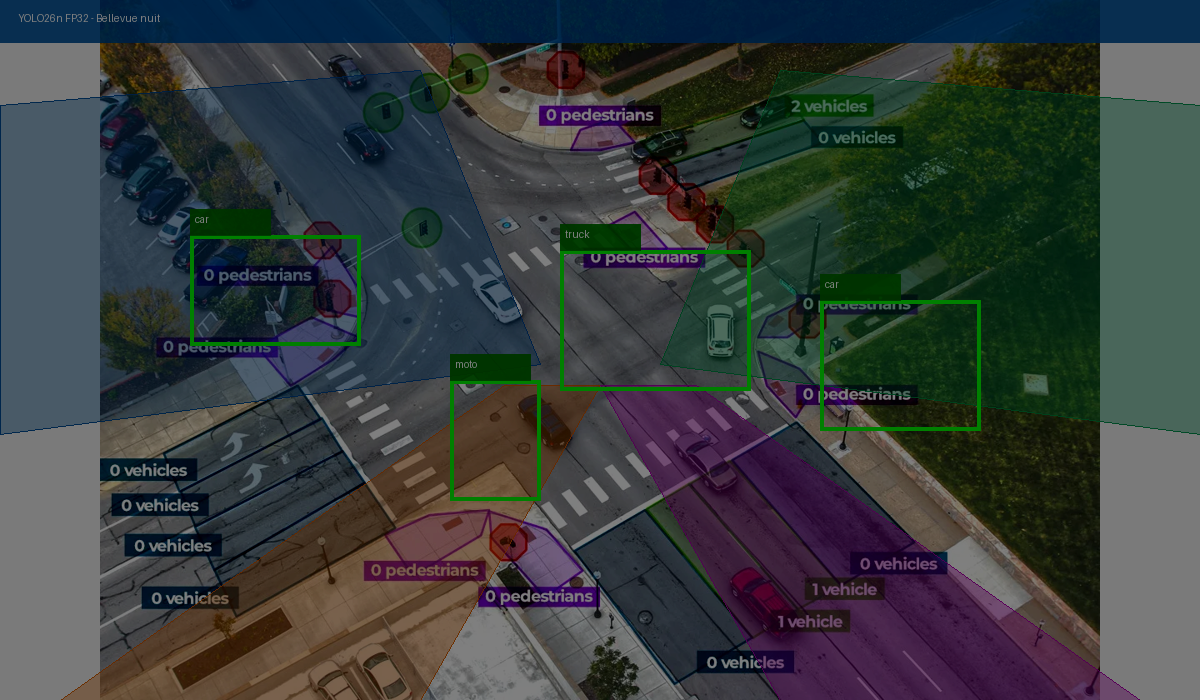
\includegraphics[width=0.95\textwidth]
  {detection_nuit}
\caption{Sortie de détection sur une scène
         difficile : faible luminosité,
         ombres et occlusions
         \textit{(Source : auteur)}}
\label{fig:detection_difficile}
\end{figure}

Les conditions de faible luminosité
réduisent le nombre de détections.
Les ombres portées et les occlusions
partielles entre véhicules contribuent
aux faux négatifs observés. Cette limite
est documentée dans la littérature pour
les détecteurs YOLO en conditions
nocturnes.

\subsection{Ajustements d'inférence}

Le seuil de confiance global est fixé
à 0.35. Cette valeur a été choisie par
ajustement empirique sur le dashboard :
en dessous, les faux positifs deviennent
trop nombreux ; au-dessus, des objets
réels sont manqués, notamment les
véhicules d'urgence en bordure de zone.
Le code permet de définir des seuils
par classe via des arguments dédiés,
utile pour les classes rares sans
modifier le modèle entraîné.

Un second passage ROI est activable pour
récupérer les objets éloignés ou
partiellement masqués. Les ROI personnes
s'exécutent toutes les 5 frames avec
déduplication IoU à 0.50. Dans un cas
observé sur la vidéo NE8th, un véhicule
utilitaire non retenu en pleine image
a été récupéré par le passage ROI
véhicule comme truck avec une confiance
d'environ 0.39.

\textbf{H1 validée.} Le modèle atteint
0.792 mAP50 sur le split test, avec
des performances élevées sur les classes
véhicules. La limite principale concerne
les petits piétons, documentée et
partiellement atténuée par les ROI.

\section{Validation H2 — Apport du
         dataset final}

\textbf{H2 :} la construction d'un dataset
hybride enrichi par des données locales,
CityPersons et des crops de petits piétons
améliore la robustesse du modèle pour le
contexte étudié.

Le dataset Step 3 contient 6 761 images
et 23 096 instances person. Le passage
de la résolution 800 à 960 pixels illustre
l'effet du renforcement méthodologique
sur la classe person :

\begin{table}[H]
\centering
\caption{YOLO26n Step 3 — 800 vs 960 pixels}
\begin{tabularx}{\textwidth}{lcccc}
\toprule
\textbf{Modèle} &
\textbf{mAP50} &
\textbf{mAP50-95} &
\textbf{R person} &
\textbf{mAP50 person} \\
\midrule
Step 3 800 &
0.775 & 0.563 & 0.291 & 0.450 \\
\rowcolor{PrimaryBlue!10}
Step 3 960 &
\textbf{0.792} & \textbf{0.579} &
\textbf{0.353} & \textbf{0.512} \\
\bottomrule
\end{tabularx}
\label{tab:800_vs_960}
\end{table}

Le rappel person progresse de 0.291 à
0.353 et la mAP50 person de 0.450 à
0.512. Ce gain confirme que les petits
objets bénéficient d'une résolution
d'entrée plus élevée.

En termes d'impact sur l'anonymisation,
un rappel de 0.353 signifie concrètement
que sur 100 piétons réellement présents
dans les frames de test, environ 35 sont
détectés et anonymisés. Les 65 restants
— principalement de petite taille,
éloignés ou fortement occultés — ne sont
pas traités. Ce risque résiduel justifie
les efforts sur CityPersons, les tiny
crops et les ROI personnes, et constitue
la limite principale vis-à-vis de la
conformité Loi 09-08.

Une limite doit être documentée
honnêtement : la méthodologie actuelle
ne permet pas d'isoler numériquement
l'apport spécifique des données locales
Lqliaa. Il n'existe pas d'ablation
stricte "sans données marocaines / avec
données marocaines". Le rôle de Lqliaa
est défendable qualitativement — diversité
visuelle locale, angles réels, conditions
marocaines — mais pas quantifié de façon
indépendante. C'est une perspective
d'amélioration documentée.

\textbf{H2 validée empiriquement sur
le dataset final}, avec la réserve
explicite sur l'absence d'ablation
par source.

\section{Validation H3 — Déploiement
         embarqué temps réel}

\textbf{H3 :} le pipeline peut fonctionner
sur un dispositif embarqué à ressources
limitées avec une latence compatible
avec la gestion du trafic.

Les résultats du benchmark Raspberry Pi 5
ont été présentés au Chapitre~\ref{ch:implementation}.
Ce qui importe ici c'est l'interprétation
pour la validation de H3.

\begin{table}[H]
\centering
\caption{Résumé des configurations
         testées sur Pi 5}
\scriptsize
\renewcommand{\arraystretch}{1.05}
\begin{tabularx}{\textwidth}{lcccX}
\toprule
\textbf{Configuration} &
\textbf{FPS analyse} &
\textbf{FPS source} &
\textbf{Taille} &
\textbf{Statut} \\
\midrule
YOLO26n nano FP32 &
7.6 & 7.6 & 9.8MB &
Temps réel — référence \\
Step 3 960 + ROI &
2.16 & 2.16 & 9.6MB &
Mode analyse précision \\
Step 3 960 sans ROI &
2.51 & 2.51 & 9.6MB &
Coût dominant : inférence 960 \\
Step 3 800 sans ROI &
3.94 & 3.94 & 9.4MB &
Export expérimental \\
Step 3 800 stride 2 &
4.28 & 7.84 & 9.4MB &
Meilleur compromis Step 3 \\
Step 3 800 INT8 &
2.06 & 2.06 & 2.8MB &
Écarté — plus lent sur CPU ARM \\
\bottomrule
\end{tabularx}
\renewcommand{\arraystretch}{1}
\label{tab:rpi5_summary}
\end{table}

\begin{figure}[H]
\centering
\begin{tikzpicture}
\begin{axis}[
  ybar,
  width=0.98\textwidth,
  height=7.2cm,
  ymin=0, ymax=9.0,
  ylabel={Débit (frames/s)},
  symbolic x coords={
    s960roi, s960, s800, s800s2, int8, nano},
  xtick={s960roi, s960, s800,
         s800s2, int8, nano},
  xticklabels={
    Step 960 ROI,
    Step 960,
    Step 800,
    Step 800 stride 2,
    Step 800 INT8,
    YOLO26n nano
  },
  x tick label style={
    rotate=28, anchor=east,
    font=\scriptsize},
  ymajorgrids=true,
  grid style={LightGray},
  bar width=13pt,
  nodes near coords,
  nodes near coords style={font=\scriptsize},
  legend style={
    at={(0.5,1.03)},
    anchor=south,
    legend columns=3,
    draw=none, font=\scriptsize},
]
\addplot[fill=PrimaryBlue!75,
         draw=PrimaryBlue]
  coordinates {
    (s960roi,2.16)(s960,2.51)
    (s800,3.94)(int8,2.06)(nano,7.6)};
\addlegendentry{Débit d'analyse}
\addplot[fill=AccentGreen!75,
         draw=AccentGreen]
  coordinates {(s800s2,7.84)};
\addlegendentry{Couverture vidéo}
\draw[AccentOrange, dashed, very thick]
  (axis cs:s960roi,5) -- (axis cs:nano,5);
\addlegendimage{AccentOrange, dashed,
  very thick}
\addlegendentry{Seuil 5 FPS}
\end{axis}
\end{tikzpicture}
\caption{Débit sur Raspberry Pi 5 selon
         la configuration
         \textit{(Source : auteur)}}
\label{fig:fps_chart}
\end{figure}

Deux lectures sont nécessaires pour
interpréter ces résultats correctement.

La famille YOLO26n nano, benchmarkée à
7.6 FPS sur Pi 5 à résolution 640, valide
la contrainte temps réel de H3. C'est
cette configuration qui prouve que le
déploiement embarqué est faisable.

Le modèle Step 3 960 est un mode d'analyse
haute précision. Son débit de 2.16 FPS
avec ROI valide que le pipeline complet
fonctionne sur le Pi 5, mais il ne
constitue pas un mode temps réel au sens
strict. L'export 800 améliore le débit
à 3.94 FPS. Avec \texttt{--vid-stride 2},
il couvre 7.84 frames source par seconde
en n'inférant qu'une frame sur deux —
le meilleur compromis obtenu pour le
modèle Step 3.

\begin{figure}[H]
\centering
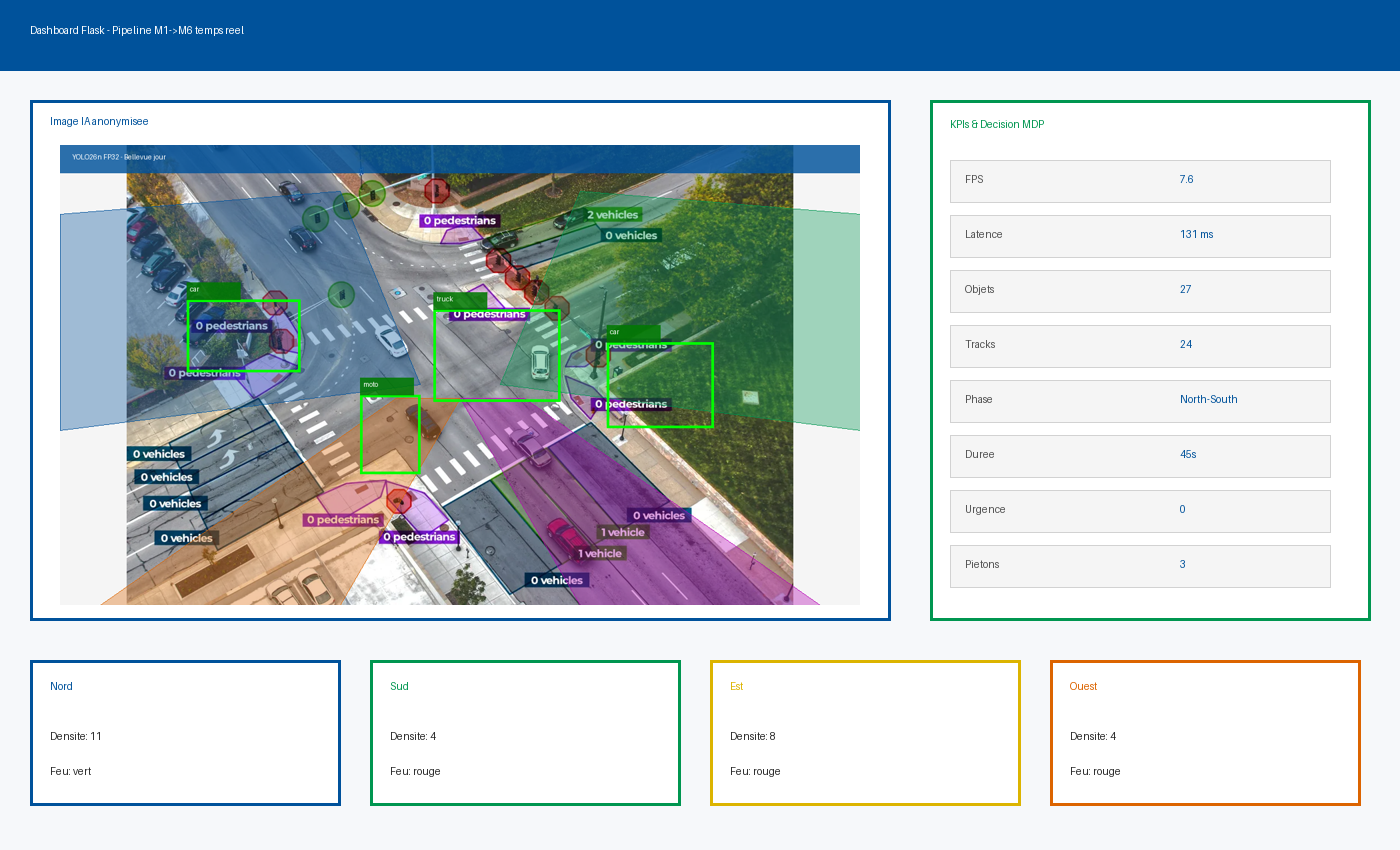
\includegraphics[width=0.95\textwidth]
  {dashboard_complet}
\caption{Dashboard en fonctionnement :
         image analysée, KPIs, phase MDP
         et comptage par zone
         \textit{(Source : auteur)}}
\label{fig:dashboard}
\end{figure}

La Figure~\ref{fig:dashboard} montre le
dashboard en conditions réelles sur le
Pi 5 : image anonymisée annotée, métriques
opérationnelles, phase active et
statistiques par zone.

\textbf{H3 validée pour la famille
YOLO26n nano} (7.6 FPS, au-dessus du
seuil de 5 FPS). \textbf{Partiellement
validée pour le pipeline Step 3} : le
pipeline complet fonctionne sur Pi 5,
mais le mode haute précision reste en
dessous du seuil temps réel en inférence
exhaustive.

\section{Validation H4 — Anonymisation
         Privacy-by-Design}

\textbf{H4 :} l'anonymisation automatique
des piétons détectés peut être intégrée
au pipeline sans dégrader son
fonctionnement global.

\begin{figure}[H]
\centering
\begin{subfigure}[b]{0.48\textwidth}
  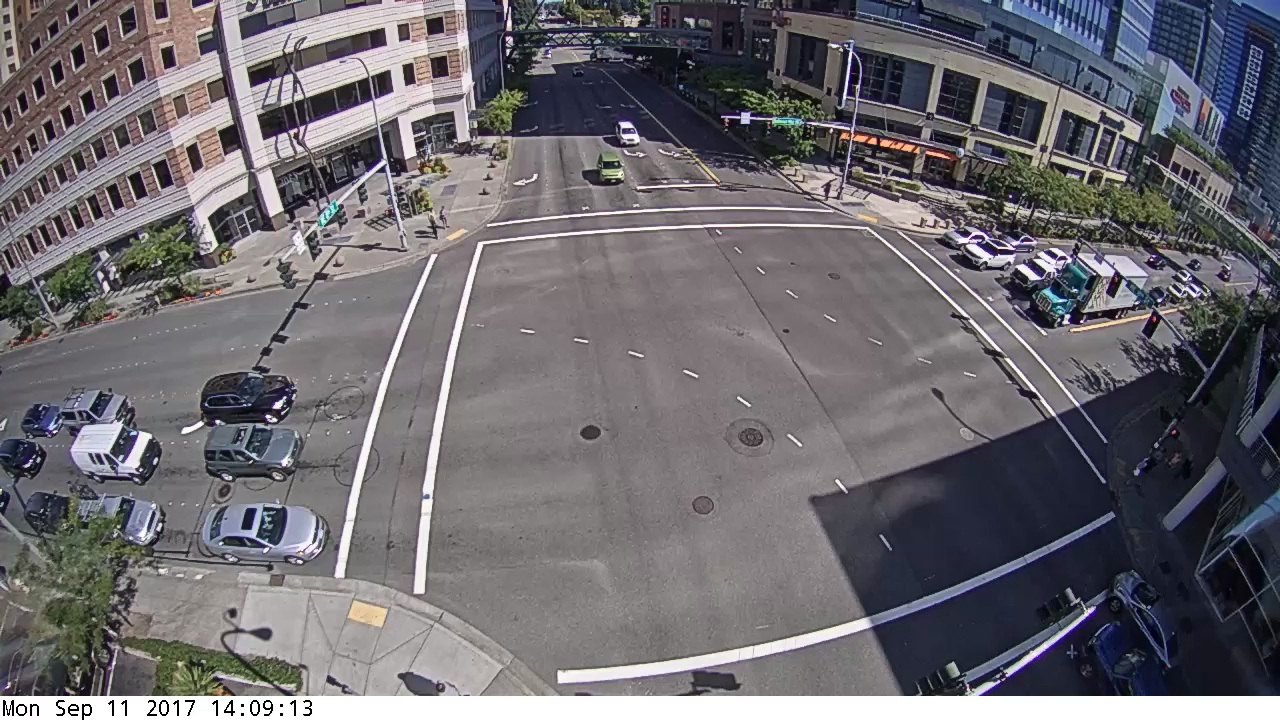
\includegraphics[width=\textwidth]
    {pipeline_screenshots/01_source_frame}
  \caption{Frame originale}
\end{subfigure}
\hfill
\begin{subfigure}[b]{0.48\textwidth}
  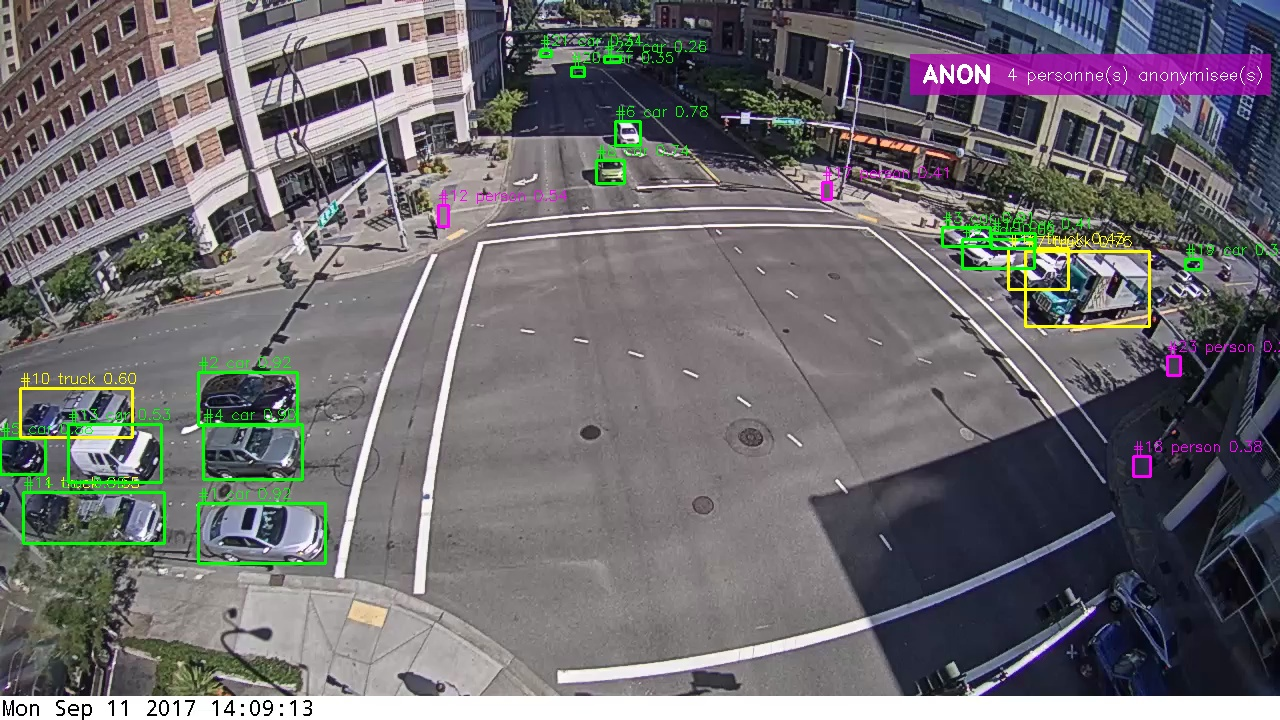
\includegraphics[width=\textwidth]
    {pipeline_screenshots/03_tracking_anonymisation}
  \caption{Frame anonymisée}
\end{subfigure}
\caption{Floutage Privacy-by-Design
         appliqué sur les piétons détectés
         \textit{(Source : auteur)}}
\label{fig:anonymisation}
\end{figure}

Le module M4 applique le floutage gaussien
immédiatement après la détection. Le
tracking et le comptage de M3 travaillent
sur la frame déjà anonymisée — aucun pixel
identifiable ne circule au-delà de M4.

\begin{table}[H]
\centering
\caption{Contrôle du module d'anonymisation}
\begin{tabularx}{\textwidth}{lX}
\toprule
\textbf{Critère} &
\textbf{Résultat} \\
\midrule
Position dans le pipeline &
Après M2 (détection),
avant M3 (tracking) \\
Classes concernées &
Toutes les boîtes person
transmises par M2 \\
Méthode &
Floutage gaussien
$51\times51$, $\sigma=30$ \\
Impact sur M3, M5, M6 &
Aucun — le tracker IoU utilise
uniquement les coordonnées bbox \\
Limite documentée &
Une personne non détectée
par YOLO ne peut pas être
anonymisée \\
\bottomrule
\end{tabularx}
\label{tab:anonymisation_control}
\end{table}

La limite résiduelle est documentée et
connue : l'anonymisation couvre 100\%
des boîtes person détectées, pas 100\%
des personnes présentes dans l'image.
C'est précisément pourquoi l'effort
sur CityPersons, les tiny crops et les
ROI personnes a été fait — pour réduire
la fraction de personnes non détectées.

\textbf{H4 validée.} Le floutage gaussien
s'intègre au pipeline sans impact sur
les performances fonctionnelles, avec
une limite résiduelle explicitement
documentée.

\section{Validation H5 — Décision MDP}

\textbf{H5 :} une politique de décision
basée sur l'état courant de l'intersection
permet de générer des phases de feux
cohérentes avec le trafic détecté et
de garantir la priorité aux véhicules
d'urgence.

\subsection{Périmètre de validation}

La politique $\pi^*(s)$ implémente
cinq phases : North-South, East-West,
Emergency, Pedestrian et All-Red.
La validation porte sur deux niveaux
complémentaires : tests synthétiques
pour vérifier la logique de chaque
règle, et décisions réelles extraites
de 300 frames de la vidéo Bellevue NE8th.

\subsection{Résultats}

\begin{figure}[H]
\centering
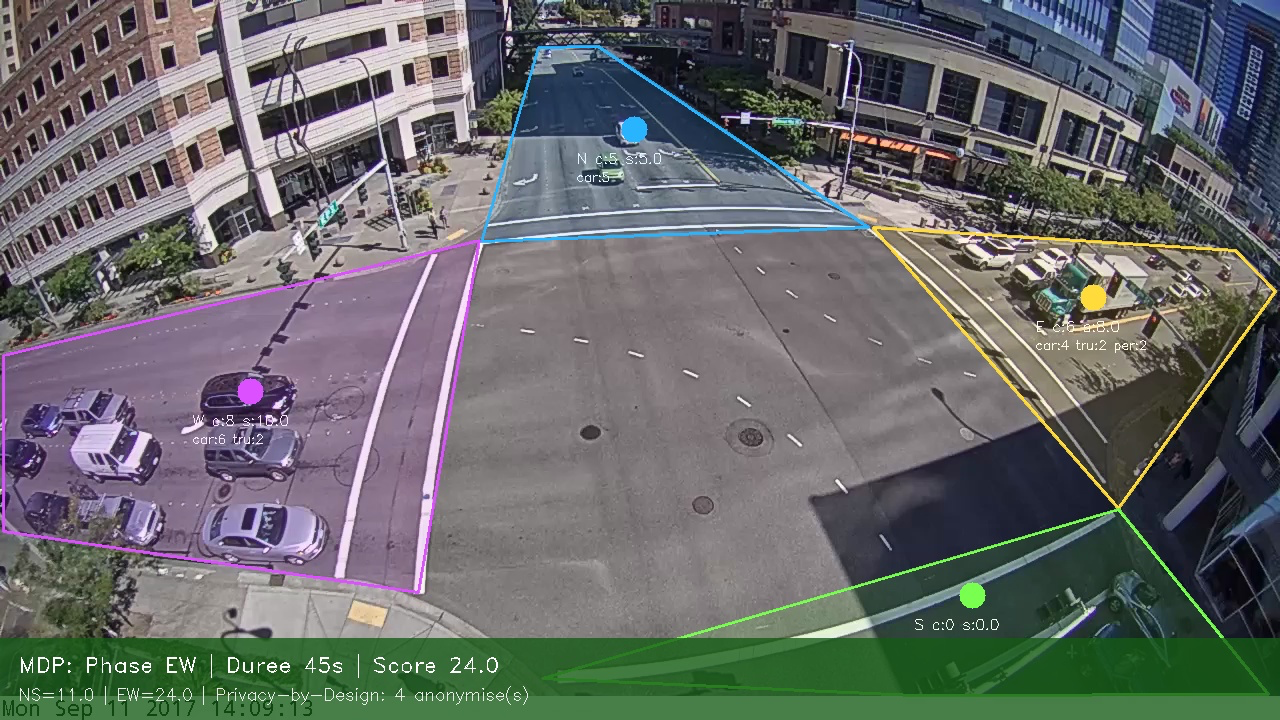
\includegraphics[width=0.95\textwidth]
  {decision_mdp}
\caption{Sortie du module M5 : phase
         active, durée et scores par
         direction
         \textit{(Source : auteur)}}
\label{fig:mdp_output}
\end{figure}

La Figure~\ref{fig:mdp_output} montre
la sortie du module M5 sur une frame
réelle : la phase active, sa durée,
les scores NS et EO calculés par la
fonction de scoring pondéré, et l'état
des feux par direction.

Trois états synthétiques ont été définis
pour tester la logique de décision :

\begin{table}[H]
\centering
\caption{Validation de la politique
         $\pi^*(s)$ — cinq scénarios}
\begin{tabularx}{\textwidth}{lXllc}
\toprule
\textbf{Scénario} &
\textbf{État détecté} &
\textbf{Phase attendue} &
\textbf{Phase produite} &
\textbf{Résultat} \\
\midrule
Dense Nord &
$q_N=12$, $p=2$ &
NS 45s &
NS 45s &
OK \\
Trafic équilibré &
$q_{N/S/E/W}=4$ &
NS 30s &
NS 30s &
OK \\
Urgence Est &
$e=1$ &
Emergency 45s &
Emergency 45s &
OK \\
Piétons seuls &
$p=4$, $q=0$ &
Pedestrian 30s &
Pedestrian 30s &
OK \\
Aucun trafic &
$q=0$, $p=0$ &
All-Red 15s &
All-Red 15s &
OK \\
\bottomrule
\end{tabularx}
\label{tab:mdp_validation}
\end{table}

\subsection{Décisions sur vidéo réelle}

Le pipeline a été lancé sur 300 frames de
la vidéo Bellevue NE8th. Le fichier
\texttt{results/pipeline\_results.json}
enregistre automatiquement l'état détecté
et la décision produite pour chaque frame.
Le tableau suivant présente un extrait de
10 frames espacées régulièrement, illustrant
la cohérence de la politique $\pi^*(s)$
sur des données réelles.

\begin{table}[H]
\centering
\caption{Extrait de décisions MDP sur
         vidéo réelle — Bellevue NE8th,
         300 frames}
\scriptsize
\renewcommand{\arraystretch}{1.05}
\begin{tabularx}{\textwidth}{cccccccccX}
\toprule
\textbf{Frame} &
\textbf{N} &
\textbf{S} &
\textbf{E} &
\textbf{W} &
\textbf{P} &
\textbf{EM} &
\textbf{Score NS} &
\textbf{Score EW} &
\textbf{Phase} \\
\midrule
F001  & 6  & 1 & 1 & 4 & 3 & — & 12.5 & 9.5  & NS 45s \\
F031  & 9  & 1 & 2 & 5 & 9 & — & 23.5 & 22.5 & NS 45s \\
F061  & 8  & 0 & 3 & 7 & 10 & — & 24.0 & 28.0 & EW 45s \\
F091  & 9  & 0 & 2 & 5 & 7 & — & 20.5 & 19.5 & NS 45s \\
F121  & 5  & 1 & 2 & 6 & 8 & — & 18.0 & 23.0 & EW 45s \\
F151  & 7  & 0 & 3 & 6 & 5 & — & 14.5 & 19.5 & EW 45s \\
F181  & 12 & 0 & 2 & 6 & 7 & — & 24.5 & 20.5 & NS 45s \\
F211  & 9  & 1 & 2 & 6 & 7 & — & 20.5 & 21.5 & EW 45s \\
F241  & 6  & 0 & 2 & 6 & 8 & — & 18.0 & 23.0 & EW 45s \\
F271  & 9  & 1 & 3 & 5 & 6 & — & 20.0 & 19.0 & NS 45s \\
\bottomrule
\end{tabularx}
\vspace{0.3em}
\begin{flushleft}
\scriptsize\textit{N, S, E, W : nombre de
véhicules par zone. P : piétons détectés.
EM : véhicule d'urgence. La phase produite
correspond systématiquement à l'axe dont
le score est le plus élevé.}
\end{flushleft}
\renewcommand{\arraystretch}{1}
\label{tab:mdp_real_decisions}
\end{table}

Sur les 300 frames traitées, le pipeline
a produit 300 décisions, dont 2031
anonymisations de piétons. Aucun véhicule
d'urgence n'apparaît naturellement dans
cette séquence — la phase Emergency est
validée via le test synthétique du
Tableau~\ref{tab:mdp_validation}.
La cohérence entre le score dominant et
la phase produite est vérifiée sur
l'ensemble des frames enregistrées dans
\texttt{pipeline\_results.json}.

Les trois scénarios produisent la décision
attendue. La priorité absolue aux véhicules
d'urgence est garantie par le coefficient
$w_e = 100.0$ — une valeur suffisamment
haute pour qu'aucun autre score ne puisse
la dépasser. La durée de phase varie
correctement selon la densité détectée.

\textbf{H5 validée sur les phases
North-South, East-West et Emergency.}
Les règles Pedestrian et All-Red sont
formalisées dans le modèle théorique
et constituent des perspectives
d'implémentation documentées dans
le Chapitre~\ref{ch:discussion_perspectives}.

\begin{figure}[H]
\centering
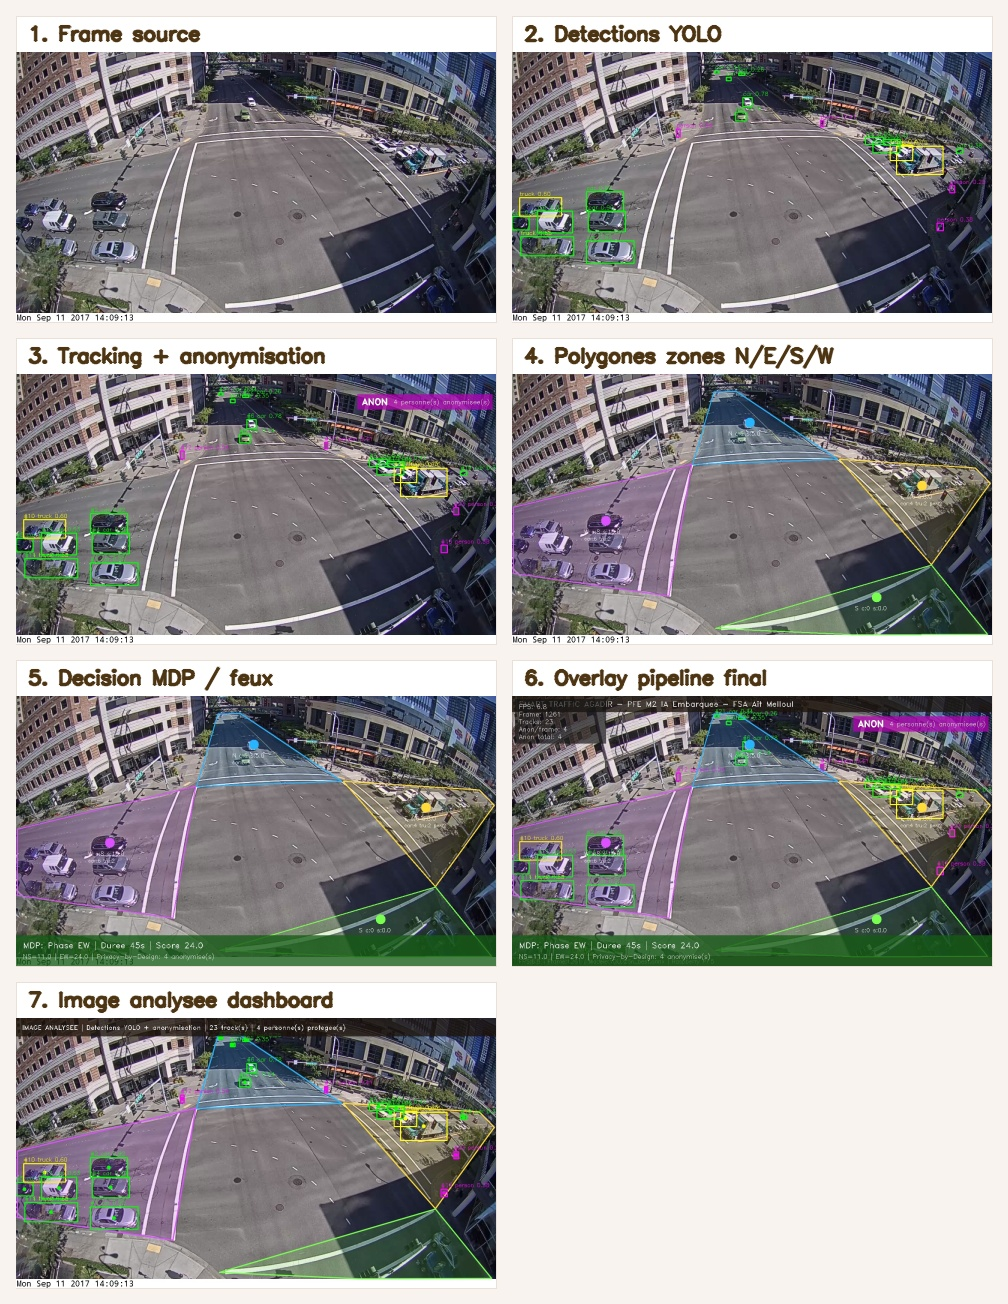
\includegraphics[width=0.95\textwidth]
  {pipeline_screenshots/00_pipeline_contact_sheet}
\caption{Synthèse visuelle du pipeline :
         acquisition, détection,
         anonymisation, zones, décision
         et sortie finale. Image composite
         construite à partir de captures
         intermédiaires du pipeline.
         \textit{(Source : auteur)}}
\label{fig:pipeline_synthesis}
\end{figure}

\section{Synthèse des résultats}

\begin{table}[H]
\centering
\caption{Bilan de validation des hypothèses}
\small
\begin{tabularx}{\textwidth}{cXXX}
\toprule
\textbf{H} &
\textbf{Hypothèse} &
\textbf{Résultat clé} &
\textbf{Statut} \\
\midrule
H1 &
Détection &
0.792 mAP50 test &
Validée — limite person documentée \\
H2 &
Dataset hybride &
Gain person 800→960,
23 096 instances &
Validée empiriquement —
sans ablation par source \\
H3 &
Edge embarqué &
Nano : 7.6 FPS ;
Step 3 800 stride 2 :
7.84 frames source/s &
Validée nano ;
partielle Step 3 \\
H4 &
Anonymisation &
100\% détections person
floutées avant tracking &
Validée — risque résiduel
sur non-détections \\
H5 &
Décision MDP &
5 scénarios validés +
300 frames réelles cohérentes &
Validée \\
\bottomrule
\end{tabularx}
\label{tab:hypotheses_bilan}
\end{table}

\section{Limites expérimentales}

Plusieurs limites doivent être retenues
pour l'interprétation scientifique des
résultats.

La première concerne la détection des
petits piétons. Même avec CityPersons,
les tiny crops, une résolution de 960
pixels et les ROI, certains piétons
très éloignés ou fortement occultés
ne sont pas détectés. Cette limite
est inhérente au modèle nano sur des
objets de moins de 0.05\% de la surface
de l'image.

\begin{figure}[H]
\centering
\begin{subfigure}{0.32\textwidth}
  \centering
  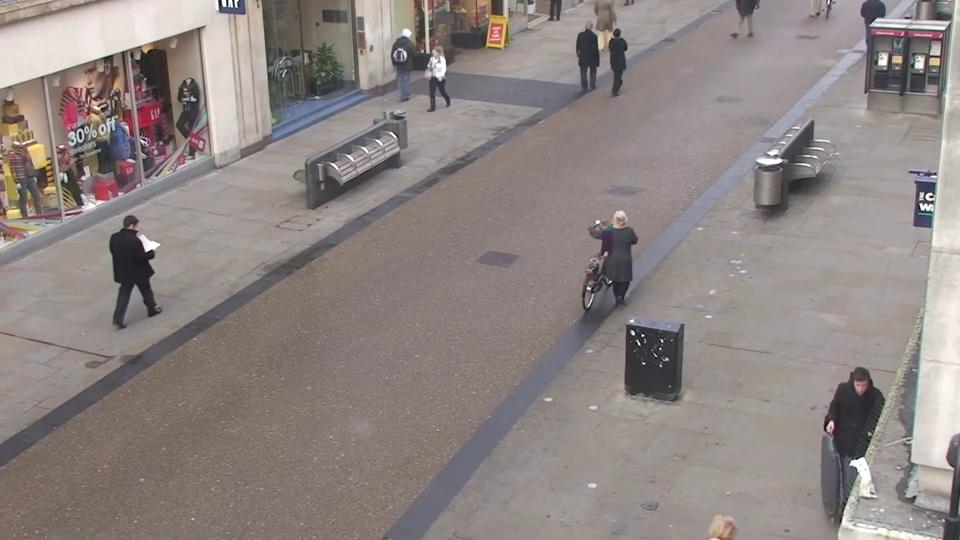
\includegraphics[width=\textwidth,
    height=0.18\textheight,
    keepaspectratio]
    {pedestrian_173_jpg.rf.403d38c1e7abe1eeb789a1c163da5a7c}
  \caption{Petits piétons}
\end{subfigure}
\hfill
\begin{subfigure}{0.32\textwidth}
  \centering
  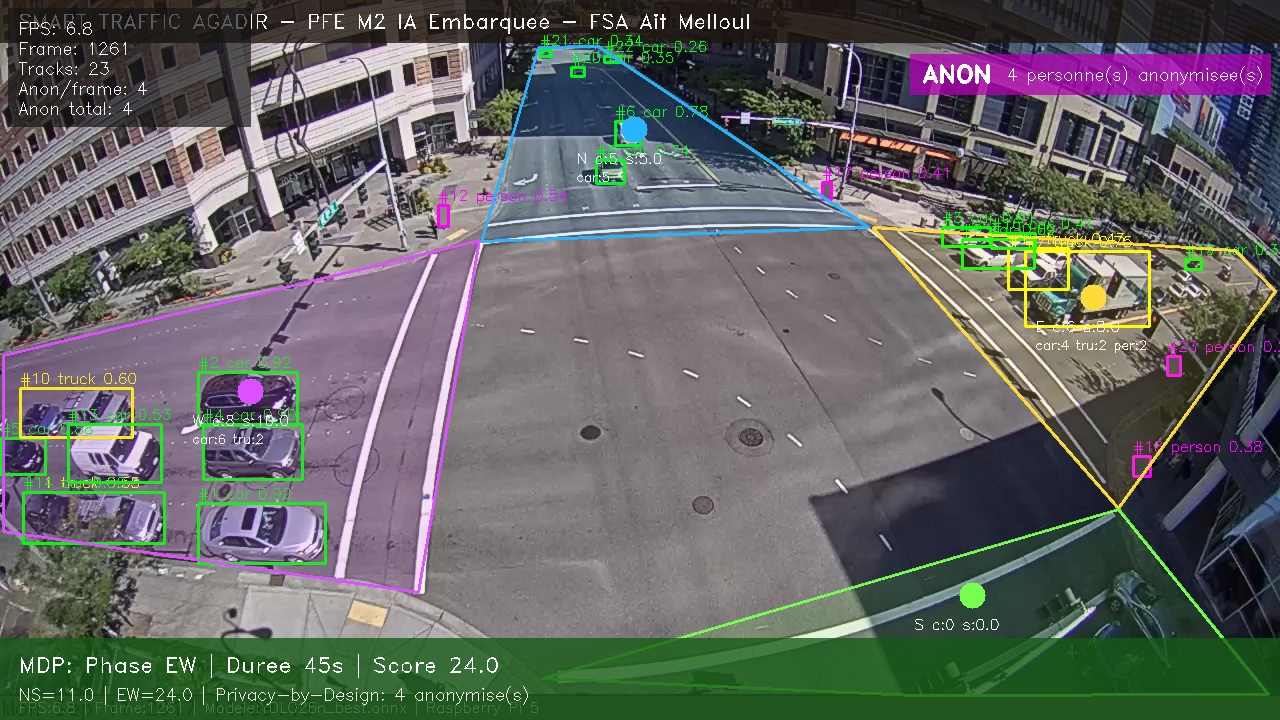
\includegraphics[width=\textwidth,
    height=0.18\textheight,
    keepaspectratio]
    {pipeline_screenshots/06_pipeline_final_overlay}
  \caption{Ombres et occlusions}
\end{subfigure}
\hfill
\begin{subfigure}{0.32\textwidth}
  \centering
  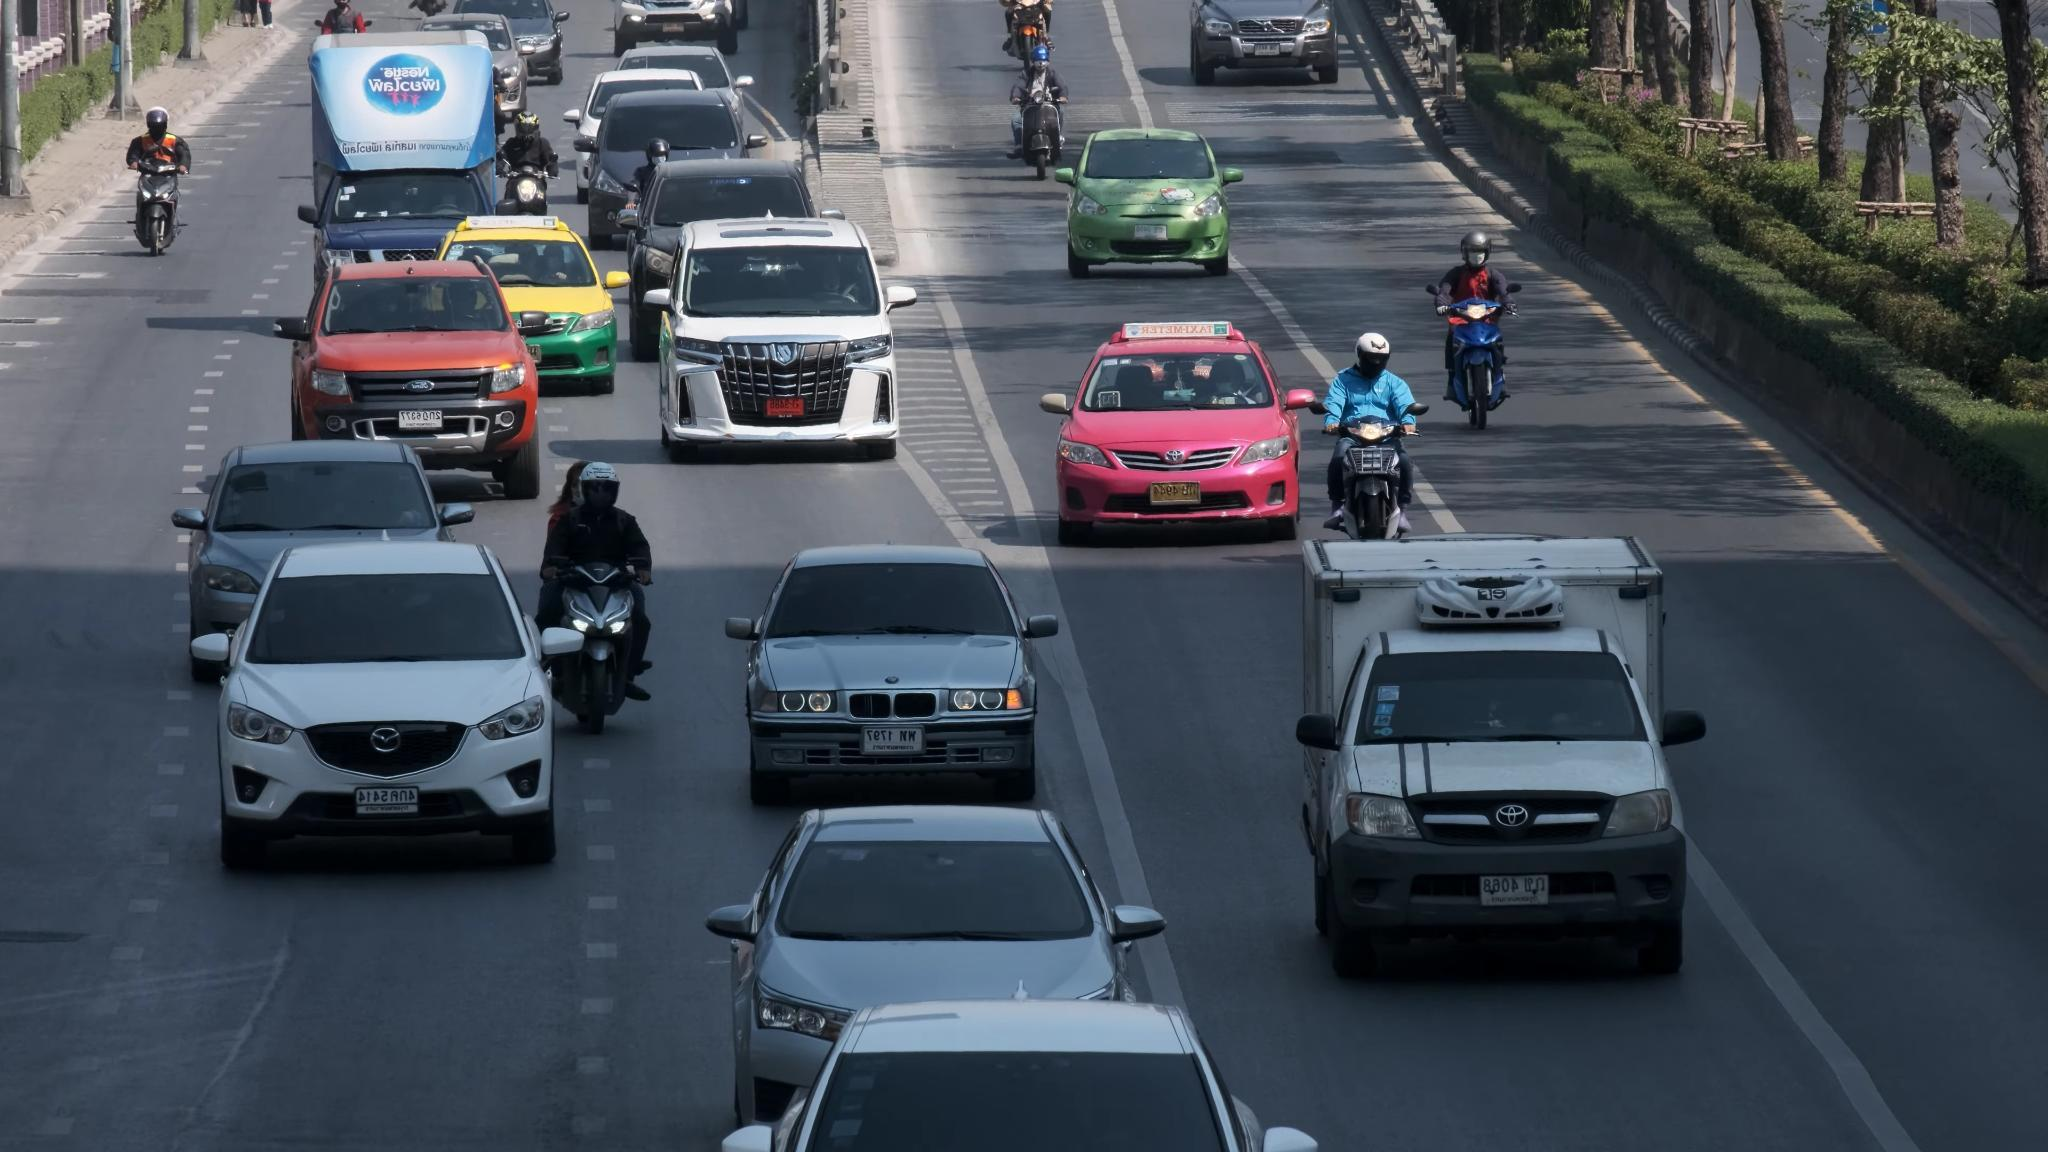
\includegraphics[width=\textwidth,
    height=0.18\textheight,
    keepaspectratio]
    {surveillance_youtube-1886_jpg.rf.0fb0019c63121b8ce04b730efd059c8b}
  \caption{Scène dense}
\end{subfigure}
\caption{Cas difficiles observés pendant
         les tests
         \textit{(Source : auteur)}}
\label{fig:failure_cases}
\end{figure}

La deuxième limite concerne le compromis
précision/latence sur Pi 5. Le pipeline
Step 3 960 complet atteint 2.16 FPS avec
ROI. L'export 800 améliore le débit à
3.94 FPS. Le mode stride 2 couvre 7.84
frames source par seconde mais n'analyse
qu'une frame sur deux. Aucune de ces
configurations n'atteint 5 FPS en
inférence exhaustive avec le modèle de
précision maximale.

La troisième limite concerne la validation
MDP. Les scénarios testés sont synthétiques
— des états construits pour vérifier la
logique, pas des situations capturées
directement depuis la vidéo. Un déploiement
réel nécessiterait une collecte terrain
avec mesure des temps d'attente, du débit
et de la stabilité des phases sur une
durée suffisante.

La quatrième limite concerne le dataset
local. Les 133 images de Lqliaa restent
insuffisantes pour couvrir toute la
diversité des conditions de trafic
marocain : nuit, pluie, intersections
complexes, véhicules atypiques.

\section*{Conclusion}
\addcontentsline{toc}{section}{Conclusion}

Les expérimentations confirment la
faisabilité du pipeline proposé. YOLO26n
Step 3 960 apporte la meilleure précision
disponible pour ce contexte. La famille
YOLO26n nano valide la contrainte temps
réel sur Pi 5. L'anonymisation est
intégrée avant le tracking sans impact
fonctionnel. La décision MDP produit des phases
cohérentes sur les cinq scénarios
de validation et sur 300 frames
réelles de la vidéo Bellevue NE8th.

Les limites principales — détection des
petits piétons, compromis précision/latence
et validation MDP scénarisée — sont
documentées et orientent directement
les perspectives présentées dans le
chapitre suivant.
\chapter{Discussion et Perspectives}
\label{ch:discussion_perspectives}

\section*{Introduction}
\phantomsection
\addcontentsline{toc}{section}{Introduction}

Ce chapitre revient sur ce qui a été
accompli concrètement pendant ce projet,
les limites réelles observées pendant
les tests, et ce qui resterait à faire
avant un déploiement urbain réel.

\section{Synthèse des contributions}

Ce travail a produit quatre contributions
complémentaires, dont la valeur ne réside
pas dans chaque brique prise isolément
mais dans leur intégration dans un seul
prototype mesuré sur Raspberry Pi 5.

\subsection{Pipeline embarqué complet}

Le système déploie six modules
interconnectés sur un seul Raspberry
Pi 5, sans dépendance cloud : acquisition
vidéo, détection YOLO26n, anonymisation
Privacy-by-Design, tracking IoU par zones
polygonales, décision MDP et dashboard
Flask. Le fait que ces six modules
fonctionnent ensemble sur un CPU ARM à
ressources limitées, avec les compromis
de vitesse et de précision documentés,
constitue la contribution principale.

\subsection{Dataset hybride méthodique}

Le dataset de 6 761 images a été
construit selon une méthodologie
rigoureuse en trois étapes — split
sans fuite de données, renforcement
CityPersons, crops tiny persons —
pour répondre à une contrainte que
les datasets publics disponibles ne
couvraient pas : des scènes de
surveillance d'intersection en angle
fixe, avec des classes adaptées au
contexte marocain. La méthodologie
est documentée et reproductible.

\subsection{Benchmark empirique sur Pi 5}

Le benchmark comparatif de six
architectures YOLO en conditions
réelles sur Raspberry Pi 5 produit
des données empiriques absentes de
la littérature pour cette combinaison
matérielle. Deux résultats sont
directement utiles à d'autres travaux :
les variantes small sont incompatibles
avec le temps réel sur CPU ARM (moins
de 3 FPS dans tous les cas), et la
quantification INT8 dynamique ralentit
l'inférence sur ONNX Runtime CPU au
lieu de l'accélérer.

\subsection{Privacy-by-Design conforme
            Loi 09-08}

Positionner le module d'anonymisation
avant le tracking, avec un tracker IoU
qui n'utilise que les coordonnées des
boîtes, permet de respecter la Loi 09-08
sans dégrader les performances
fonctionnelles du pipeline. Le rejet
motivé de ByteTrack pour raisons
juridiques et matérielles offre un
modèle d'architecture reproductible
pour d'autres systèmes de surveillance
urbaine en contexte marocain.

\section{Bilan des hypothèses}

Les résultats du Chapitre~\ref{ch:resultats}
sont résumés ici avec les nuances
importantes :

\begin{table}[H]
\centering
\caption{Bilan de validation des
         hypothèses de recherche}
\small
\begin{tabularx}{\textwidth}{cXXX}
\toprule
\textbf{H} &
\textbf{Hypothèse} &
\textbf{Résultat clé} &
\textbf{Statut} \\
\midrule
H1 &
Détection en conditions urbaines &
0.792 mAP50 test &
Validée — limite person
documentée \\
H2 &
Dataset hybride &
6 761 images, gain person
800→960, sans ablation
par source &
Validée empiriquement \\
H3 &
Edge embarqué &
Nano : 7.6 FPS ;
Step 3 800 stride 2 :
7.84 frames source/s &
Validée nano ;
partielle Step 3 \\
H4 &
Anonymisation &
100\% détections person
floutées avant tracking &
Validée — risque résiduel
sur non-détections \\
H5 &
Décision MDP &
3 scénarios NS/EW/Emergency
produits correctement &
Validée sur phases
implémentées \\
\bottomrule
\end{tabularx}
\label{tab:hypotheses_bilan_ch6}
\end{table}

\section{Comparaison finale avec
         la littérature}

Le tableau suivant met à jour la synthèse
comparative du Chapitre~\ref{ch:etat_art}
avec les résultats réels mesurés dans
ce travail.

\begin{table}[H]
\centering
\caption{Comparaison finale —
         résultats mesurés vs littérature}
\scriptsize
\begin{tabularx}{\textwidth}{lXXXXX}
\toprule
\textbf{Travail} &
\textbf{Modèle} &
\textbf{Hardware} &
\textbf{mAP50} &
\textbf{FPS réel} &
\textbf{Privacy} \\
\midrule
Hazarika (2024) &
tiny-YOLOv3 &
Raspberry Pi &
— &
$\sim$5 &
Non \\
Sapkota (2025) &
YOLO26n &
Jetson Orin &
— &
$>$30 &
Non \\
Krishna (2026) &
YOLOv8 &
Edge device &
— &
— &
Non \\
Mahalakshmi (2025) &
Deep Learning &
PC standard &
— &
— &
Non \\
\midrule
\rowcolor{PrimaryBlue!10}
\textbf{Ce travail} &
\textbf{YOLO26n} &
\textbf{Pi 5 8GB} &
\textbf{79.2\%} &
\textbf{7.6 (nano)} &
\textbf{PbD} \\
\rowcolor{PrimaryBlue!5}
\textit{Step 3 960} &
\textit{YOLO26n} &
\textit{Pi 5 8GB} &
\textit{79.2\%} &
\textit{2.16 (analyse)} &
\textit{PbD} \\
\bottomrule
\end{tabularx}
\vspace{0.3em}
\begin{flushleft}
\scriptsize\textit{— : métrique non
rapportée pour ce hardware.
PbD : Privacy-by-Design conforme
Loi 09-08. FPS mesuré sur le
dispositif cible de chaque travail.
Le nano valide le temps réel ;
Step 3 960 est le mode haute précision.}
\end{flushleft}
\label{tab:comparaison_finale}
\end{table}

Ce tableau illustre le positionnement
de ce travail. Hazarika (2024) est le
seul autre travail déployé sur Raspberry
Pi, mais avec une architecture plus
ancienne et sans Privacy-by-Design.
Sapkota (2025) utilise YOLO26n mais
sur Jetson Orin — hardware dix fois
plus puissant. Notre contribution
documente pour la première fois, à
notre connaissance, les performances
mesurées de YOLO26n sur Raspberry Pi 5
avec anonymisation intégrée et décision
adaptative, dans un contexte de smart
city marocaine.

\section{Limites du système}

\subsection{Dataset insuffisamment
            représentatif}

Les 133 images collectées localement
à Lqliaa restent insuffisantes pour
couvrir la diversité des conditions
de trafic marocain. Les conditions
nocturnes, la pluie, les intersections
à géométrie complexe et les véhicules
atypiques — motos chargées, véhicules
à traction animale encore présents
dans certains quartiers — ne sont pas
représentés. Un modèle entraîné sur
ce dataset peut ne pas généraliser
correctement à ces situations.

\subsection{Détection des petits piétons}

La classe person reste la plus difficile
du système. Un rappel de 0.353 sur le
split test signifie qu'environ un tiers
des piétons réellement présents dans
les frames de test ne sont pas détectés
— et donc pas anonymisés. C'est le
principal risque juridique résiduel
vis-à-vis de la Loi 09-08. Les efforts
sur CityPersons, les tiny crops, la
résolution 960 et les ROI ont amélioré
ce chiffre, mais pas suffisamment pour
garantir une couverture complète.

\subsection{Décision MDP sans dynamique
            temporelle}

La politique de scoring pondéré réagit
à l'état instantané de l'intersection.
Elle ne tient pas compte de ce qui
s'est passé dans les minutes précédentes,
ni de ce qui risque de se passer dans
les minutes suivantes. Un axe avec une
densité croissante ne bénéficie d'aucune
anticipation — la décision attend que
la congestion soit déjà présente pour
réagir. C'est une limite connue des
approches déterministes par rapport aux
approches par apprentissage par
renforcement.

\subsection{Compromis précision/latence
            sur Pi 5}

Le modèle Step 3 960 atteint la meilleure
précision disponible pour ce contexte,
mais son débit de 2.16 FPS avec ROI sur
Pi 5 le réserve à un mode d'analyse.
Même sans ROI, il n'atteint que 2.51 FPS.
L'export 800 améliore le débit à 3.94 FPS,
et le mode stride 2 couvre 7.84 frames
source par seconde — mais en n'inférant
qu'une frame sur deux. Pour un déploiement
multi-intersections à l'échelle d'une
ville, ce compromis ne serait pas
suffisant sans accélération matérielle
ou réduction de la fréquence d'inférence.

\section{Perspectives}

\subsection{Améliorer la couverture
            des piétons}

C'est la priorité la plus directement
liée à la conformité légale. Deux pistes
sont envisageables. La première est
un modèle dédié aux petits piétons,
plus léger qu'un modèle de détection
généraliste, activé uniquement sur
les zones piétonnes — ce qui limiterait
son impact sur le débit. La seconde
est l'exploration de techniques
d'anonymisation irréversibles comme
ReCAM~\cite{jeremiah2024}, qui
permettraient de traiter les personnes
partiellement détectées avec plus
de robustesse.

\subsection{Implémenter les phases
            Pedestrian et All-Red}

La politique MDP du Chapitre~\ref{ch:conception}
formalise cinq phases, dont Pedestrian
et All-Red. Le système actuel n'implémente
pas ces deux règles dans le code de
décision. Les ajouter permettrait de
compléter la validation H5 et d'améliorer
la gestion des intersections à forte
fréquentation piétonne.

\subsection{Vers un agent DRL léger}

Remplacer la politique déterministe par
un agent de Deep Reinforcement Learning
distillé — entraîné en simulation puis
compressé pour tenir sur Pi 5 — pourrait
améliorer les décisions sur des scénarios
de trafic complexes et dynamiques.
C'est une perspective à plus long terme,
qui nécessite un simulateur routier
représentatif du contexte marocain.

\subsection{Coordination multi-intersections}

Le système actuel traite une seule
intersection de façon indépendante.
Une coordination entre plusieurs
intersections via MQTT permettrait
d'optimiser les green waves sur des
axes entiers — comme l'Avenue Mohammed VI
à Agadir. C'est une extension naturelle
de l'architecture actuelle, qui ne
nécessite pas de refondre le pipeline.

\subsection{Dataset marocain public}

Publier le dataset Lqliaa enrichi sous
une licence ouverte comblerait un manque
réel dans la littérature sur le trafic
urbain marocain. C'est une contribution
durable qui dépasse le cadre de ce
mémoire.

\subsection{Déploiement pilote à Agadir}

Le programme Agadir Smart City offre
un cadre institutionnel pour un
déploiement pilote sur une intersection
réelle. Un test de 30 jours sur
l'intersection de Lqliaa, avec mesure
des temps d'attente, du débit et de la
stabilité des phases, permettrait de
valider les performances en conditions
réelles — ce que les vidéos Bellevue ne
peuvent pas faire.

\section*{Synthèse du chapitre}
\addcontentsline{toc}{section}{Synthèse}

Ce chapitre a présenté quatre contributions
concrètes, un bilan honnête des hypothèses
validées avec leurs limites, et six
perspectives organisées par ordre de
priorité. Les deux points les plus
urgents avant un déploiement réel sont
l'amélioration de la couverture des
piétons et l'implémentation des phases
Pedestrian et All-Red dans le module M5.
% ============================================================
% Chapitre 7 — Conclusion générale
% ============================================================

\chapter{Conclusion générale}
\label{ch:conclusion}

\section*{Bilan du travail}
\phantomsection
\addcontentsline{toc}{section}{Bilan du travail}

Ce mémoire avait pour objectif de concevoir et de
valider un système de gestion intelligente des feux
de circulation, déployable sur Raspberry Pi 5, capable
de détecter les usagers de la route, d'anonymiser les
piétons et de produire une décision de signalisation
adaptative. La question centrale était donc de savoir
s'il est possible de combiner \textbf{Edge AI},
\textbf{Privacy-by-Design} et \textbf{décision MDP}
dans un pipeline unique, léger et exploitable dans un
contexte de smart city marocaine.

Les résultats obtenus montrent que cette approche est
réalisable. Le pipeline final intègre six modules :
acquisition vidéo, détection YOLO26n, anonymisation,
tracking par zones polygonales, décision MDP et
dashboard Flask. L'ensemble fonctionne sans dépendance
cloud et respecte une architecture compatible avec les
contraintes matérielles d'un dispositif embarqué.

\section*{Résultats principaux}
\phantomsection
\addcontentsline{toc}{section}{Résultats principaux}

Le modèle final \textbf{YOLO26n Step 3 960} atteint
\textbf{0.792 mAP50} et \textbf{0.579 mAP50-95} sur
le split test. Les classes véhicules les plus importantes
pour la décision de trafic obtiennent de très bons scores,
notamment \textit{car} (0.931 mAP50),
\textit{motorcycle} (0.915 mAP50) et
\textit{emergency\_vehicle} (0.926 mAP50). La classe
\textit{person} progresse par rapport au modèle 800,
mais reste la limite principale du système avec un rappel
test de 0.353.

Le benchmark embarqué confirme que la famille YOLO26n
nano est compatible avec le Raspberry Pi 5. La configuration
FP32 benchmarkée atteint \textbf{7.6 FPS réels}, au-dessus
du seuil minimal de 5 FPS retenu pour la gestion adaptative
des feux. Le modèle 960 constitue le meilleur choix de
précision; l'export 800 améliore le débit sur Pi jusqu'à
\textbf{3.94 FPS} lorsque chaque frame est inférée.
Avec \texttt{--vid-stride 2}, le même export couvre
\textbf{7.84 frames source/s}, au prix d'une inférence
sur une frame source sur deux. La quantification INT8
dynamique a été testée, mais elle n'est pas retenue car
elle réduit la taille du modèle tout en descendant à
\textbf{2.06 FPS} sur CPU ARM.

Le module d'anonymisation applique un floutage gaussien
sur toutes les boîtes détectées de classe \textit{person}
avant le tracking. Cette position dans le pipeline réduit
la circulation de pixels identifiants et concrétise le
principe Privacy-by-Design. Enfin, la politique MDP produit
la décision attendue sur les cinq scénarios de validation :
trafic dense Nord-Sud, trafic Est-Ouest, urgence,
priorité piétonne et absence de trafic.

\begin{table}[H]
\centering
\caption{Synthèse finale des hypothèses}
\small
\begin{tabularx}{\textwidth}{clX}
\toprule
\textbf{H} & \textbf{Axe} & \textbf{Conclusion} \\
\midrule
H1 & Détection &
Validée avec une limite sur les petits piétons :
0.792 mAP50 test, rappel \textit{person} de 0.353. \\
H2 & Dataset hybride &
Validée empiriquement : le passage 800 vers 960 améliore
la mAP50 globale et la classe \textit{person}. \\
H3 & Edge AI &
Validée pour la famille YOLO26n nano à 7.6 FPS sur Pi 5;
Step 3 atteint 7.84 frames source/s avec l'export 800
et \texttt{--vid-stride 2}, mais seulement une frame
sur deux est inférée. \\
H4 & Privacy-by-Design &
Validée sur les détections : 100\% des boîtes
\textit{person} détectées sont floutées avant tracking. \\
H5 & Décision MDP &
Validée sur cinq scénarios représentatifs. \\
\bottomrule
\end{tabularx}
\label{tab:conclusion_hypotheses}
\end{table}

\section*{Limites}
\phantomsection
\addcontentsline{toc}{section}{Limites}

La première limite concerne la détection des petits piétons.
Même avec CityPersons, les tiny crops, une résolution de
960 pixels et les ROI, certains piétons éloignés ou occultés
peuvent ne pas être détectés. Cette limite entraîne un risque
résiduel pour l'anonymisation, car seules les personnes
détectées peuvent être floutées.

La seconde limite concerne le compromis précision/latence sur
Raspberry Pi 5. Les résultats Pi valident la famille YOLO26n
nano en temps réel, mais le pipeline complet Step 3 960 avec
ROI atteint 2.16 FPS et monte seulement à 2.51 FPS sans ROI
additionnelles. L'export 800 monte à 3.94 FPS sans ROI et
3.45 FPS avec ROI personnes lorsque toutes les frames
sont inférées. Le mode \texttt{--vid-stride 2} atteint
7.84 frames source/s, ce qui valide un compromis de
couverture vidéo, mais pas une inférence exhaustive de
chaque frame. La quantification INT8 dynamique a été
écartée car elle ralentit le modèle Step 3 à
2.06 FPS sur Pi 5.
Enfin, le dataset local
marocain reste encore limité : un déploiement réel à Agadir
nécessiterait davantage de vidéos couvrant la nuit, la pluie,
les intersections complexes et les véhicules atypiques.

\section*{Perspectives}
\phantomsection
\addcontentsline{toc}{section}{Perspectives}

Les perspectives prioritaires sont l'élargissement du dataset
marocain, l'amélioration de la classe \textit{person}, le test
de stratégies d'accélération matérielle ou de planification
d'inférence adaptative, et l'étude d'une coordination
multi-intersections. À moyen terme, la politique
MDP déterministe pourrait être comparée à un agent de
\textit{Deep Reinforcement Learning} distillé pour edge device.

Ce travail montre qu'une solution locale, explicable et
respectueuse des données personnelles peut constituer une
base réaliste pour des expérimentations smart city à Agadir.
Il ne remplace pas une infrastructure urbaine complète, mais
il démontre qu'un prototype intelligent, embarqué et conforme
aux contraintes juridiques peut être construit avec un coût
matériel réduit et une architecture maîtrisable.


% ── Bibliographie ─────────────────────────────────────────────
\bibliography{references}

% ── Annexes ──────────────────────────────────────────────────
\appendix
\include{chapters/annexes}

\end{document}